\NumberThisInToc
\chapter{Renommage dans une séquence répliquée}
\minitoc
\label{chap:renamablelogootsplit}

\section{Présentation de l'approche}
Nous proposons un nouveau \ac{CRDT} pour le type Séquence appartenant à l'approche à identifiants densément ordonnés et à granularité variable : RenamableLogootSplit \cite{2020-rls-papoc-nicolas,2022-rls-tpds-nicolas}.
Cette structure de données permet aux noeuds d'insérer et de supprimer des éléments au sein d'une séquence répliquée.
Nous introduisons une opération de renommage qui permet de :
\begin{enumerate}
  \item Réassigner des identifiants plus courts aux différents éléments de la séquence.
  \item Fusionner les blocs composant la séquence.
\end{enumerate}
Ces deux actions permettent à l'opération de renommage de produire un nouvel état minimisant son surcoût en termes de métadonnées et de calculs des modifications suivantes.


\subsection{Définition de l'opération de renommage}
\label{sec:def-rename-op}

L'objectif de l'opération \emph{rename} est de réassigner de nouveaux identifiants aux éléments de la séquence répliquée sans modifier son contenu.
Puisque les identifiants sont des métadonnées utilisées par la structure de données uniquement afin de résoudre les conflits, les utilisateurs ignorent leur existence.
Les opérations \emph{rename} sont donc des opérations systèmes : elles sont émises et appliquées par les noeuds en coulisses, sans aucune intervention des utilisateurs.

Afin de garantir le respect du modèle de cohérence \ac{SEC}, nous définissons plusieurs propriétés de sécurité que l'opération \emph{rename} doit respecter.
Ces propriétés sont inspirées principalement par celles proposées dans \cite{zawirski:hal-01248197}.

\begin{property}(Déterminisme)
  Les opérations \emph{rename} sont intégrées par les noeuds sans aucune coordination.
  Pour assurer que l'ensemble des noeuds atteigne un état équivalent à terme, une opération \emph{rename} donnée doit toujours générer le même nouvel identifiant à partir de l'identifiant courant.
\end{property}

\begin{property}(Préservation de l'intention de l'utilisateur)
  Bien que l'opération \emph{rename} n'est pas elle-même n'incarne pas une intention de l'utilisateur, elle ne doit pas entrer en conflit avec les actions des utilisateurs.
  Notamment, les opérations \emph{rename} ne doivent pas annuler ou altérer le résultat d'opérations \emph{insert} et \emph{remove} du point de vue des utilisateurs.
\end{property}

\begin{property}(Séquence bien formée)
  La séquence répliquée doit être bien formée.
  Appliquée une opération \emph{rename} sur une séquence bien formée doit produire une nouvelle séquence bien formée.
  Une séquence bien formée doit respecter les propriétés suivantes :
  \begin{itemize}[noitemsep]
    \item[~]
    \begin{subproperty}(Préservation de l'unicité)
      Chaque identifiant doit être unique.
      Donc, pour une opération \emph{rename} donnée, chaque identifiant doit être associé à un nouvel identifiant distinct.
    \end{subproperty}
    \item[~]
    \begin{subproperty}(Préservation de l'ordre)
      \label{prop:order}
      Les éléments de la séquence doivent être triés en fonction de leur identifiants.
      L'ordre existant entre les identifiants initiaux doit donc être préservé par l'opération \emph{rename}.
    \end{subproperty}
  \end{itemize}
\end{property}

\begin{property}(Commutativité avec les opérations concurrentes)
  \label{prop:commutativity}
  Les opérations concurrentes peuvent être livrées dans des ordres différents à chaque noeud.
  Afin de garantir la convergence des réplicas, l'ordre d'application d'un ensemble d'opérations concurrentes ne doit pas avoir d'impact sur l'état obtenu.
  L'opération \emph{rename} doit donc être commutative avec n'importe quelle opération concurrente.
\end{property}

La \autoref{prop:commutativity} est particulièrement difficile à assurer.
Cette difficulté est dûe au fait que les opérations \emph{rename} modifient les identifiants assignés aux éléments.
Cependant, les autres opérations telles que les opérations \emph{insert} et \emph{remove} reposent sur ces identifiants pour spécifier où insérer les éléments ou lesquels supprimer.
Les opérations \emph{rename} sont donc intrinséquement incompatibles avec les opérations \emph{insert} et \emph{remove} concurrentes.
De la même manière, des opérations \emph{rename} concurrentes peuvent réassigner des identifiants différents à des mêmes éléments.
Les opérations \emph{rename} concurrentes ne sont donc pas commutatives.
Par conséquent, il est nécessaire de concevoir et d'utiliser des méthodes de résolution de conflits pour assurer la \autoref{prop:commutativity}.

Dans un souci de simplicité, la présentation de l'opération \emph{rename} est divisée en deux parties.
Dans le \autoref{sec:centralised-rls}, nous présentons l'opération \emph{rename} proposée avec l'hypothèse qu'aucune opération \emph{rename} concurrente ne peut être générée.
Cette hypothèse nous permet de nous concentrer sur le fonctionnement de l'opération \emph{rename} elle-même ainsi que sur comment gérer les opérations \emph{insert} et \emph{remove} concurrentes.
Ensuite, dans le \autoref{sec:distributed-rls}, nous supprimons cette hypothèse.
Nous présentons alors notre approche pour gérer les scénarios avec des opérations \emph{rename} concurrentes.


\section{Introduction de l'opération $\trm{rename}$}
\label{sec:centralised-rls}

\subsection{Opération de renommage proposée}
L'opération $\trm{rename}$, abrégée en $\trm{ren}$ dans nos figures, réassigne des identifiants arbitraires aux éléments de la séquence de réduire son surcoût en métadonnées.

\begin{figure}[t!]
  \centering
  \subfloat[Choix du nouvel identifiant pour le premier élément]{
      \begin{minipage}{\linewidth}
          \centering
          \resizebox{0.7 \columnwidth}{!}{
          \begin{tikzpicture}
            \newcommand\nodeh[1]{
                node[letter, label=#1:{$\betterid{i}{B1}{0}$}] {H}
            }
            \newcommand\nodee[1]{
                node[letter, fill=\colorblockone, label=#1:{$\coloridone\betterid{i}{B1}{0}\betterid{f}{A1}{0}$}] {E}
            }
            \newcommand\nodelo[1]{
                node[block, label=#1:{$\betterid{i}{B1}{1..2}$}] {LO}
            }
            \newcommand\renh[1]{
                node[letter, fill=\colorblocktwo, label=#1:{$\coloridtwo\betterid{i}{A2}{0}$}] {H}
            }

            \newcommand\initialstate[3]{
                \path
                #1
                ++#2
                ++(0:0.5)
                ++(#3:0.5) \nodeh{-#3}
                ++(0:\widthletter) \nodee{#3}
                ++(0:\widthletter) \nodelo{-#3};
            }

            \newcommand\finalstate[3]{
                \path
                #1
                ++#2
                ++(0:0.5)
                ++(#3:0.5) \renh{-#3};
            }

            \newcommand\offseta{ (90:0.7) }

            \path
                node {\textbf{A}}
                ++(0:0.5) node (a) {}
                +(0:14) node (a-end) {}
                +(0:2) node[point] (a-initial) {}
                +(0:8) node[point, label=-170:{$\trm{ren}()$}, label={[xshift=0pt]-10:{$\trm{ren}(A,2)$}}] (a-ren-a1) {}
                +(0:12) node (a-final) {};

            \initialstate{(a-initial)}{\offseta}{90};
            \finalstate{(a-ren-a1)}{\offseta}{90};

            \draw[dotted] (a) -- (a-initial) (a-final) -- (a-end);
            \draw[->, thick] (a-initial) --  (a-ren-a1) -- (a-final);
          \end{tikzpicture}}
          \label{fig:renaming-first-id}
      \end{minipage}}
  \hfil
  \subfloat[Choix des nouveaux identifiants pour les éléments restants]{
      \begin{minipage}{\linewidth}
          \centering
          \resizebox{0.7 \columnwidth}{!}{
          \begin{tikzpicture}
            \newcommand\nodeh[1]{
                node[letter, label=#1:{$\betterid{i}{B1}{0}$}] {H}
            }
            \newcommand\nodee[1]{
                node[letter, fill=\colorblockone, label=#1:{$\coloridone\betterid{i}{B1}{0}\betterid{f}{A1}{0}$}] {E}
            }
            \newcommand\nodelo[1]{
                node[block, label=#1:{$\betterid{i}{B1}{1..2}$}] {LO}
            }
            \newcommand\renh[1]{
                node[letter, fill=\colorblocktwo, label=#1:{$\coloridtwo\betterid{i}{A2}{0}$}] {H}
            }
            \newcommand\rene[1]{
                node[letter, fill=\colorblocktwo, label=#1:{$\coloridtwo\betterid{i}{A2}{1}$}] {E}
            }
            \newcommand\renl[1]{
                node[letter, fill=\colorblocktwo, label=#1:{$\coloridtwo\betterid{i}{A2}{2}$}] {L}
            }
            \newcommand\reno[1]{
                node[letter, fill=\colorblocktwo, label=#1:{$\coloridtwo\betterid{i}{A2}{3}$}] {O}
            }

            \newcommand\initialstate[3]{
                \path
                #1
                ++#2
                ++(0:0.5)
                ++(#3:0.5) \nodeh{-#3}
                ++(0:\widthletter) \nodee{#3}
                ++(0:\widthletter) \nodelo{-#3};
            }

            \newcommand\finalstate[3]{
                \path
                #1
                ++#2
                ++(0:0.5)
                ++(#3:0.5) \renh{-#3}
                ++(0:\widthletter) \rene{-#3}
                ++(0:\widthletter) \renl{-#3}
                ++(0:\widthletter) \reno{-#3};
            }

            \newcommand\offseta{ (90:0.7) }

            \path
                node {\textbf{A}}
                ++(0:0.5) node (a) {}
                +(0:14) node (a-end) {}
                +(0:2) node[point] (a-initial) {}
                +(0:8) node[point, label=-170:{$\trm{ren}()$}, label={[xshift=0pt]-10:{$\trm{ren}(A,2)$}}] (a-ren-a1) {}
                +(0:12) node (a-final) {};

            \initialstate{(a-initial)}{\offseta}{90};
            \finalstate{(a-ren-a1)}{\offseta}{90};

            \draw[dotted] (a) -- (a-initial) (a-final) -- (a-end);
            \draw[->, thick] (a-initial) --  (a-ren-a1) -- (a-final);
          \end{tikzpicture}}
          \label{fig:renaming-second-id}
      \end{minipage}}
  \hfil
  \subfloat[État final obtenu]{
      \begin{minipage}{\linewidth}
          \centering
          \resizebox{0.7 \columnwidth}{!}{
          \begin{tikzpicture}
            \newcommand\nodeh[1]{
                node[letter, label=#1:{$\betterid{i}{B1}{0}$}] {H}
            }
            \newcommand\nodee[1]{
                node[letter, fill=\colorblockone, label=#1:{$\coloridone\betterid{i}{B1}{0}\betterid{f}{A1}{0}$}] {E}
            }
            \newcommand\nodelo[1]{
                node[block, label=#1:{$\betterid{i}{B1}{1..2}$}] {LO}
            }
            \newcommand\renhelo[1]{
                node[block, fill=\colorblocktwo, label=#1:{$\coloridtwo\betterid{i}{A2}{0..3}$}] {HELO}
            }

            \newcommand\initialstate[3]{
                \path
                #1
                ++#2
                ++(0:0.5)
                ++(#3:0.5) \nodeh{-#3}
                ++(0:\widthletter) \nodee{#3}
                ++(0:\widthletter) \nodelo{-#3};
            }

            \newcommand\finalstate[3]{
                \path
                #1
                ++#2
                ++(0:0.5)
                ++(#3:0.5) \renhelo{-#3};
            }

            \newcommand\offseta{ (90:0.7) }

            \path
                node {\textbf{A}}
                ++(0:0.5) node (a) {}
                +(0:14) node (a-end) {}
                +(0:2) node[point] (a-initial) {}
                +(0:8) node[point, label=-170:{$\trm{ren}()$}, label={[xshift=0pt]-10:{$\trm{ren}(A,2)$}}] (a-ren-a1) {}
                +(0:12) node (a-final) {};

            \initialstate{(a-initial)}{\offseta}{90};
            \finalstate{(a-ren-a1)}{\offseta}{90};

            \draw[dotted] (a) -- (a-initial) (a-final) -- (a-end);
            \draw[->, thick] (a-initial) --  (a-ren-a1) -- (a-final);
          \end{tikzpicture}}
          \label{fig:renaming-final-state}
      \end{minipage}}
  \caption{Renommage de la séquence sur le noeud \emph{A}}
  \label{fig:renaming}
\end{figure}

Son comportement est illustré dans la \autoref{fig:renaming}.
Dans cet exemple, le noeud A initie une opération $\trm{rename}$ sur son état local.
Tout d'abord, le noeud A génère un nouvel identifiant à partir du premier tuple de l'identifiant du premier élément de la séquence (\id{i}{B1}{0}).
Pour générer ce nouvel identifiant, le noeud A reprend la position de ce tuple (\emph{i}) mais utilise son propre identifiant de noeud (\textbf{A}) et numéro de séquence actuel ($2$).
De plus, son offset est mis à 0.
Le noeud A réassigne l'identifiant résultant (\id{i}{A2}{0}) au premier élément de la séquence, comme décrit dans la \autoref{fig:renaming-first-id}.
Ensuite, le noeud A dérive des identifiants contigus pour tous les éléments restants en incrémentant de manière successive l'offset (\id{i}{A2}{1}, \id{i}{A2}{2}, \id{i}{A2}{3}), comme présenté dans la \autoref{fig:renaming-second-id}.
Comme nous assignons des identifiants consécutifs à tous les éléments de la séquence, nous pouvons au final aggréger ces éléments en un seul bloc, comme illustré en \autoref{fig:renaming-final-state}.
Ceci permet aux noeuds de bénéficier au mieux de la fonctionnalité des blocs et de minimiser le surcoût en métadonnés de l'état résultat.\\

Pour converger, les autres noeuds doivent renommer leur état de manière identique.
Cependant, ils ne peuvent pas simplement remplacer leur état courant par l'état généré par le renommage.
En effet, ils peuvent avoir modifié en concurrence leur état.
Afin de ne pas perdre ces modifications, les noeuds doivent traiter l'opération $\trm{rename}$ eux-mêmes.
Pour ce faire, le noeud qui a généré l'opération $\trm{rename}$ diffuse les données sur lesquelles il a basé son renommage aux autres, \ie son \emph{ancien état}.

\begin{definition}[Ancien état]
  \label{def:former-state}
  Un \emph{ancien état} est la liste des intervalles d'identifiants qui composent l'état courant de la séquence répliquée au moment du renommage.
\end{definition}

De ce fait, nous définissons l'opération $\trm{rename}$ de la manière suivante :

\begin{definition}[rename]
  \label{def:rename-op}
  Une opération $\trm{rename}$ est un triplet $\langle \trm{nodeId}, \trm{nodeSeq}, \trm{formerState} \rangle$ où
  \begin{enumerate}
    \item $\trm{nodeId}$ est l'identifiant du noeud qui a généré l'opération $\trm{rename}$.
    \item $\trm{nodeSeq}$ est le numéro de séquence du noeud au moment de la génération de l'opération $\trm{rename}$.
    \item $\trm{formerState}$ est l'ancien état du noeud au moment du renommage.
  \end{enumerate}
\end{definition}

En utilisant ces données, les autres noeuds calculent le nouvel identifiant de chaque identifiant renommé.
Concernant les identifiants insérés de manière concurrente au renommage, nous expliquons dans la \autoref{sec:ops-concurrent-to-rename} comment les noeuds peuvent les renommer de manière déterministe.


\subsection{Gestion des opérations concurrentes au renommage}
\label{sec:ops-concurrent-to-rename}

Après avoir appliqué des opérations \emph{rename} sur leur état local, les noeuds peuvent recevoir des opérations concurrentes.
La \autoref{fig:concurrent-insert-rename-inconsistent} illustre de tels cas.

\begin{figure}[!ht]
  \centering
  \resizebox{\columnwidth}{!}{
    \begin{tikzpicture}
        \path
            node {\textbf{A}}
            ++(0:\widthletter) node[letter, label=below:{\id{i}{B0}{0}}] {H}
            ++(0:\widthletter) node[letter, fill=mydarkorange, label=above:{\color{mydarkorange}\id{i}{B0}{0}\id{f}{\,A0}{0}}] {E}
            ++(0:\widthletter) node[block, label=below:{\id{i}{B0}{1..2}}] (S0A-right) {LO}
            ++(0:5 * \widthletter) node[block, fill=mydarkblue,
                    label={below:{\color{mydarkblueid}\id{i}{A1}{0..3}} }
                        ] (S1A) {HELO}
            ++(0:8 * \widthletter) node[block, fill=mydarkblue,
                    label={below:{\color{mydarkblueid}\id{i}{A1}{0..3}} }
                        ] (S2A-left) {HELO}
            ++(0:1.18 * \widthblock) node[letter, fill=mylightorange, cross,
                    label={above:{\color{mylightorange}\id{i}{B0}{0}\id{m}{B1}{0}} }
                        ] {L};

        \path
            ++(270:2) node {\textbf{B}}
            ++(0:\widthletter) node[letter, label=below:{\id{i}{B0}{0}}] {H}
            ++(0:\widthletter) node[letter, fill=mydarkorange, label=above:{\color{mydarkorange}\id{i}{B0}{0}\id{f}{\,A0}{0}}] {E}
            ++(0:\widthletter) node[block, label=below:{\id{i}{B0}{1..2}}] (S0B-right) {LO}
            ++(0:5 * \widthletter) node[letter, label=below:{\id{i}{B0}{0}}] (S1B-left) {H}
            ++(0:\widthletter) node[letter, fill=mydarkorange, label=above:{\color{mydarkorange}\id{i}{B0}{0}\id{f}{\,A0}{0}}] {E}
            ++(0:\widthletter) node[letter, fill=mylightorange, label=below:{\color{mylightorange}\id{i}{B0}{0}\id{m}{B1}{0}}] {L}
            ++(0:\widthletter) node[block, label=above:{\id{i}{B0}{1..2}}] (S1B-right) {LO};


        \draw[->, thick] (S0A-right) -- node[above, align=center]{\emph{rename}} (S1A);
        \draw[dotted] (S1A) -- (S2A-left);
        \draw[->, thick] (S0B-right) -- node[below, align=center]{\emph{insert "L"}\\\emph{between}\\\emph{"E" and "L"}} (S1B-left);
        \draw[dashed, ->, thick, shorten >= 3] (S1B-right.east) -- node[below right, align=center]{\emph{insert "L" at} {\color{mylightorange}\id{i}{B0}{0}\id{m}{B1}{0}}} (S2A-left.west);

    \end{tikzpicture}
  }
  \caption{Modifications concurrentes menant à une anomalie}
  \label{fig:concurrent-insert-rename-inconsistent}
\end{figure}

Dans cet exemple, le noeud B insère un nouvel élément "L", lui assigne l'identifiant \id{i}{B0}{0}\id{m}{B1}{0} et diffuse cette modification, de manière concurrente à l'opération \emph{rename} décrite dans la \autoref{fig:concurrent-insert-rename-inconsistent}.
À la réception de l'opération \emph{insert}, le noeud A ajoute l'élément inséré au sein de sa séquence, en utilisant l'identifiant de l'élément pour déterminer sa position.
Cependant, puisque les identifiants ont été modifiés par l'opération \emph{rename} concurrente, le noeud A insère le nouvel élément à la fin de sa séquence (puisque \id{i}{A1}{3} $\lid$ \id{i}{B0}{0}\id{m}{B1}{0}) au lieu de l'insérer à la position souhaitée.
Comme illustré par cet exemple, appliquer naivement les modifications concurrentes provoquerait des anomalies.
Il est donc nécessaire de traiter les opérations concurrentes aux opérations \emph{rename} de manière particulière.

Tout d'abord, les noeuds doivent détecter les opérations concurrentes aux opérations \emph{rename}.
Pour cela, nous utilisons un système basé sur des \emph{époques}.
Initialement, la séquence répliquée débute à l'époque \emph{origine} notée \epoch{0}.
Chaque opération \emph{rename} introduit une nouvelle époque et permet aux noeuds d'y avancer depuis l'époque précédente.
Par exemple, l'opération \emph{rename} décrite dans la \autoref{fig:concurrent-insert-rename-inconsistent} permet aux noeuds de faire progresser leur état de \epoch{0} à \epoch{A1}.
Nous définissons les époques de la manière suivante :

\begin{definition}[Époque]
  Une époque est un couple $\langle \trm{nodeId}, \trm{nodeSeq} \rangle$ où
  \begin{itemize}
    \item $\trm{nodeId}$ est l'identifiant du noeud qui a généré cette époque.
    \item $\trm{nodeSeq}$ est le numéro de séquence du noeud au moment de la génération de cette époque.
  \end{itemize}
\end{definition}

Notons que l'époque générée est caractérisée et identifiée de manière unique par son couple $\langle \trm{nodeId}, \trm{nodeSeq} \rangle$.

Au fur et à mesure que les noeuds reçoivent des opérations \emph{rename}, ils construisent et maintiennent localement la \emph{chaîne des époques}.
Cette structure de données ordonne les époques en fonction de leur relation \emph{parent-enfant} et associe à chaque époque l'\emph{ancien état} correspondant (\ie l'\emph{ancien état} inclus dans l'opération \emph{rename} qui a généré cette époque).
De plus, les noeuds marquent chaque opération avec leur époque courante au moment de génération de l'opération.
À la réception d'une opération, les noeuds comparent l'époque de l'opération à l'époque courante de leur séquence.

Si les époques diffèrent, les noeuds doivent transformer l'opération avant de pouvoir l'intégrer.
Les noeuds déterminent par rapport à quelles opérations \emph{rename} doit être transformée l'opération reçue en calculant le chemin entre l'époque de l'opération et leur époque courante en utilisant la \emph{chaîne des époques}.

Les noeuds utilisent la fonction \textsc{renameId}, décrite dans l'\autoref{alg:renameId}, pour transformer les opérations \emph{insert} et \emph{remove} par rapport aux opérations \emph{rename}.
Cet algorithme associe les identifiants d'une époque \emph{parente} aux identifiants correspondant dans l'époque \emph{enfant}.
L'idée principale de cet algorithme est de renommer les identifiants inconnus au moment de la génération de l'opération \emph{rename} en utilisant leur prédecesseur.
Un exemple est présenté dans la \autoref{fig:concurrent-insert-rename-fixed}.
Cette figure décrit le même scénario que la \autoref{fig:concurrent-insert-rename-inconsistent}, à l'exception que le noeud A utilise \textsc{renameId} pour renommer l'identifiants généré de façon concurrente avant de l'insérer dans son état.

\begin{algorithm}[!ht]
  \footnotesize
  \begin{algorithmic}
      \Function {renameId}{id $\in \mathbb{I}$, renamedIds $\in \trm{Arr}\langle \mathbb{I}\rangle$, nodeId $\in \mathbb{N}$, nodeSeq $\in \mathbb{N}$}
          \Statex \Comment $\text{renamedIds} = [\text{id}_0, \text{id}_1, \cdots, \text{id}_{n-2}, \text{id}_{n-1}]$
          % \State \Comment{$id$ is the id to rename}
          % \State \Comment{$renamedIds$ is the list of ids of the \emph{former state}}
          % \State \Comment{$nId$ is $node~id$ of the node that issued the \emph{rename} op}
          % \State \Comment{$nSeq$ is $node~seq$ of the node that issued the \emph{rename} op}
          \State $\text{firstId} \gets \text{id}_0$
          \State $\text{lastId} \gets \text{id}_{n - 1}$
          \Statex \Comment $\text{firstId} = \langle \text{pos}, \_, \_, \_ \rangle \oplus \text{suffix}$
          \\
          \If{$\text{id} \lid \text{firstId}$}
              \State $\text{newFirstId} \gets \newFirstId$
              \State \Return renIdLessThanFirstId(id, newFirstId)
          \ElsIf{$\text{id} \in \text{renamedIds}$}
              \Statex \Comment $\text{id} = \text{id}_i$
              \State \Return $\langle \text{pos}, \text{nodeId}, \text{nodeSeq}, i \rangle$
          \ElsIf{$\text{lastId} \lid \text{id}$}
              \State $\text{newLastId} \gets \langle \text{pos}, \text{nodeId}, \text{nodeSeq}, n-1 \rangle$
              \State \Return renIdGreaterThanLastId(id, newLastId)
          \Else
              \State \Return renIdFromPredId(id, renamedIds, pos, nodeId, nodeSeq)
          \EndIf
      \EndFunction
      \\
      \Function {renIdFromPredId}{id $\in \mathbb{I}$, renamedIds $\in \trm{Arr} \langle \mathbb{I} \rangle$, pos $\in \mathbb{N}$, nodeId $\in \mathbb{N}$, nodeSeq $\in \mathbb{N}$}
          \Statex \Comment $\text{renamedIds} = [\text{id}_0, \text{id}_1, \cdots, \text{id}_{n-2}, \text{id}_{n-1}]$
          \State Find $\text{id}_i \in \text{renamedIds such that id}_i \lid \text{id} \lid \text{id}_{i+1}$
          \State $\text{newPredId} \gets \langle \text{pos}, \text{nodeId}, \text{nodeSeq}, i \rangle$
          \State \Return $\text{newPredId} \oplus \text{id}$
      \EndFunction
  \end{algorithmic}
  \caption{Fonctions principales pour renommer un identifiant}
  \label{alg:renameId}
\end{algorithm}

\begin{figure}[!ht]
  \centering
  \resizebox{\columnwidth}{!}{
    \begin{tikzpicture}
        \path
            node {\textbf{A}}
            ++(0:0.5 * \widthletter) node[epoch] {\epoch{0}}
            ++(0:1.05 * \widthoriginepoch) node[letter, label=below:{\id{i}{B0}{0}}] {H}
            ++(0:\widthletter) node[letter, fill=mydarkorange, label=above:{\color{mydarkorange}\id{i}{B0}{0}\id{f}{\,A0}{0}}] {E}
            ++(0:\widthletter) node[block, label=below:{\id{i}{B0}{1..2}}] (S0A-right) {LO}
            ++(0:5 * \widthletter) node[epoch] (S1A-left) {\epoch{A1}}
            ++(0:1.3 * \widthepoch) node[block, fill=mydarkblue,
                    label={below:{\color{mydarkblueid}\id{i}{A1}{0..3}} }
                        ] (S1A-right) {HELO}
            ++(0:8 * \widthletter) node[epoch] (S2A-left) {\epoch{A1}}
            ++(0:1.3 * \widthepoch) node[block, fill=mydarkblue,
                    label={below:{\color{mydarkblueid}\id{i}{A1}{0..1}} }
                        ] {HE}
            ++(0:\widthblock) node[letter, fill=mylightblue,
                    label={above:{\color{mylightblue!20!mydarkblueid}\id{i}{A1}{1}\id{i}{B0}{0}\id{m}{B1}{0}} }
                        ] {L}
            ++(0:\widthletter) node[block, fill=mydarkblue,
                    label={below:{\color{mydarkblueid}\id{i}{A1}{2..3}} }
                        ] {LO};

        \path
            ++(270:2) node {\textbf{B}}
            ++(0:0.5 * \widthletter) node[epoch] {\epoch{0}}
            ++(0:1.05 * \widthoriginepoch) node[letter, label=below:{\id{i}{B0}{0}}] {H}
            ++(0:\widthletter) node[letter, fill=mydarkorange, label=above:{\color{mydarkorange}\id{i}{B0}{0}\id{f}{\,A0}{0}}] {E}
            ++(0:\widthletter) node[block, label=below:{\id{i}{B0}{1..2}}] (S0B-right) {LO}
            ++(0:5 * \widthletter) node[epoch] (S1B-left) {\epoch{0}}
            ++(0:1.05 * \widthoriginepoch) node[letter, label=below:{\id{i}{B0}{0}}] {H}
            ++(0:\widthletter) node[letter, fill=mydarkorange, label=above:{\color{mydarkorange}\id{i}{B0}{0}\id{f}{\,A0}{0}}] {E}
            ++(0:\widthletter) node[letter, fill=mylightorange, label=below:{\color{mylightorange}\id{i}{B0}{0}\id{m}{B1}{0}}] {L}
            ++(0:\widthletter) node[block, label=above:{\id{i}{B0}{1..2}}] (S1B-right) {LO};


        \draw[->, thick] (S0A-right) -- node[above, align=center]{\emph{rename to \epoch{A1}}} (S1A-left);
        \draw[dotted] (S1A-right) -- (S2A-left);
        \draw[->, thick] (S0B-right) -- node[below, align=center]{\emph{insert "L"}\\\emph{between}\\\emph{"E" and "L"}} (S1B-left);
        \draw[dashed, ->, thick, shorten >= 3] (S1B-right.east) -- node[below right, align=center]{\emph{insert "L" at} {\color{mylightorange}\id{i}{B0}{0}\id{m}{B1}{0}}} (S2A-left.west);

    \end{tikzpicture}
  }
  \caption{Renommage de la modification concurrente avant son intégration en utilisant \textsc{renameId} afin de maintenir l'ordre souhaité}
  \label{fig:concurrent-insert-rename-fixed}
\end{figure}

L'algorithme procède de la manière suivante.
Tout d'abord, le noeud récupère le prédecesseur de l'identifiant donné \id{i}{B0}{0}\id{m}{B1}{0} dans l'ancien état : \id{i}{B0}{0}\id{f}{A0}{0}.
Ensuite, il calcule l'équivalent de \id{i}{B0}{0}\id{f}{A0}{0} dans l'état renommé : \id{i}{A1}{1}.
Finalement, le noeud A concatène cet identifiant et l'identifiant donné pour générer l'identifiant correspondant dans l'époque \emph{enfant} : \id{i}{A1}{1}\id{i}{B0}{0}\id{m}{B1}{0}.
En réassignant cet identifiant à l'élément inséré de manière concurrente, le noeud A peut l'insérer à son état tout en préservant l'ordre souhaité.

\textsc{renameId} permet aussi aux noeuds de gérer le cas contraire : intégrer des opérations \emph{rename} distantes sur leur copie locale alors qu'ils ont précédemment intégré des modifications concurrentes.
Ce cas correspond à celui du noeud B dans la \autoref{fig:concurrent-insert-rename-fixed}.
À la réception de l'opération \emph{rename} du noeud A, le noeud B utilise \textsc{renameId} sur chacun des identifiants de son état pour le renommer et atteindre un état équivalent à celui du noeud A.

L'\autoref{alg:renameId} présente seulement le cas principal de \textsc{renameId}, \ie le cas où l'identifiant à renommer appartient à l'intervalle des identifiants formant l'ancien état ($\trm{firstId} \leq_{id} \trm{id} \leq_{id} \trm{lastId}$).
Les fonctions pour gérer les autres cas, \ie les cas où l'identifiant à renommer n'appartient pas à cet intervalle ($\trm{id} <_{id} \trm{firstId}$ ou $\trm{lastId} <_{id} \trm{id}$), sont présentées dans l'\autoref{app:rename-id}.

Nous notons que l'algorithme que nous présentons ici permet aux noeuds de renommer leur état identifiant par identifiant.
Une extension possible est de concevoir \textsc{renameBlock}, une version améliorée qui renomme l'état bloc par bloc.
\textsc{renameBlock} réduirait le temps d'intégration des opérations \emph{rename}, puisque sa complexité en temps ne dépendrait plus du nombre d'identifiants (\ie du nombre d'éléments) mais du nombre de blocs.
De plus, son exécution réduirait le temps d'intégration des prochaines opérations \emph{rename} puisque le mécanisme de renommage regroupe les éléments en moins de blocs.


\subsection{Évolution du modèle de livraison des opérations}
\label{sec:renamablelogootsplit-delivery-model}

L'introduction de l'opération \emph{rename} nécessite de faire évoluer le modèle de livraison des opérations associé à RenamableLogootSplit.
Afin d'illustrer cette nécessité, considérons l'exemple suivant :

\begin{figure}[!ht]
  \centering
  \resizebox{\columnwidth}{!}{
    \begin{tikzpicture}
        \path
            node {\textbf{A}}
            ++(0:0.5 * \widthletter) node[epoch] {\epoch{0}}
            ++(0:1.05 * \widthoriginepoch) node[letter, label=below:{\id{i}{B0}{0}}] {A}
            ++(0:\widthletter) node[letter, label=below:{\id{l}{C0}{0}}] {B}
            ++(0:\widthletter) node[letter, label=below:{\id{t}{A0}{0}}] {C}
            ++(0:\widthletter) node[letter, label=below:{\id{y}{D0}{0}}] (S0A-right) {D}

            ++(0:5 * \widthletter) node[epoch] (S1A-left) {\epoch{A1}}
            ++(0:1.3 * \widthepoch) node[block, fill=mydarkblue,
                    label={below:{\color{mydarkblueid}\id{i}{A1}{0..3}} }
                        ] (S1A-right) {ABCD}

            ++(0:5 * \widthletter) node[epoch] (S2A-left) {\epoch{A1}}
            ++(0:1.3 * \widthepoch) node[block, fill=mydarkblue,
                    label={below:{\color{mydarkblueid}\id{i}{A1}{0..1}} }
                        ] {AB}
            ++(0:\widthblock) node[letter, fill=mylightblue,
                    label={above:{\color{mylightblue!20!mydarkblueid}\id{i}{A1}{1}\id{f}{A2}{0}} }
                        ] {X}
            ++(0:\widthletter) node[block, fill=mydarkblue,
                    label={below:{\color{mydarkblueid}\id{i}{A1}{2..3}} }
                        ] (S2A-right) {CD};

        \path
            ++(270:2) node {\textbf{B}}
            ++(0:0.5 * \widthletter) node[epoch] {\epoch{0}}
            ++(0:1.05 * \widthoriginepoch) node[letter, label=below:{\id{i}{B0}{0}}] {A}
            ++(0:\widthletter) node[letter, label=below:{\id{l}{C0}{0}}] {B}
            ++(0:\widthletter) node[letter, label=below:{\id{t}{A0}{0}}] {C}
            ++(0:\widthletter) node[letter, label=below:{\id{y}{D0}{0}}] (S0B-right) {D}

            ++(0:21 * \widthletter) node (S1B) {?};

        \path
          ++(270:1)
          ++ (0:14 * \widthletter) node[cross] (fail) {};

        \draw[->, thick] (S0A-right) -- node[above, align=center]{\emph{rename to \epoch{A1}}} (S1A-left);
        \draw[->, thick] (S1A-right) -- node[above, align=center]{\emph{insert "X"}\\\emph{between}\\\emph{"B" and "C"}} (S2A-left);
        \draw[dotted] (S0B-right) -- (S1B);
        \draw[dashed, ->, thick, shorten >= 3] (S1A-right.east) -- (fail);
        \draw[dashed, ->, thick, shorten >= 3] (S2A-right.east) -- node[right, align=center]{\emph{insert "X" at} {\color{mylightblue!20!mydarkblueid}\id{i}{A1}{1}\id{f}{A2}{0}}} (S1B.west);

    \end{tikzpicture}
  }
  \caption{Livraison d'une opération \emph{insert} sans avoir reçu l'opération \emph{rename} précédente}
  \label{fig:rls-invalid-delivery-order}
\end{figure}

Dans la \autoref{fig:rls-invalid-delivery-order}, les noeuds A et B répliquent tous deux une même séquence, contenant les éléments "ABCD".
Tout d'abord, le noeud A procède au renommage de cet état.
Puis il insère un nouvel élément, "X", entre "B" et "C".
Les opérations correspondantes aux actions du noeud A sont diffusées sur le réseau.

Cependant, l'opération \emph{rename} n'est pas livrée au noeud B, par exemple suite à un problème réseau.
L'opération \emph{insert} est quant à elle correctement livrée à ce dernier.
Le noeud B doit alors intégrer dans son état un élément et l'identifiant qui lui est attaché.
Mais cet identifiant est issu d'une époque (\epoch{A1}) différente de son époque actuelle (\epoch{0}) et dont le noeud n'avait pas encore connaissance.
Il convient de s'interroger sur l'état à produire dans cette situation.

Comme nous l'avions déjà illustré par la \autoref{fig:concurrent-insert-rename-inconsistent}, les identifiants d'une époque ne peuvent être comparés qu'aux identifiants de la même époque.
Tenter d'intégrer une opération \emph{insert} ou \emph{remove} provenant d'une époque encore inconnue ne résulterait qu'en un état incohérent et une transgression de l'intention utilisateur.
Il est donc nécessaire d'empêcher ce scénario de se produire.

Pour cela, nous proposons de faire évoluer le modèle de livraison des opérations de RenamableLogootSplit.
Celui-ci repose sur celui de LogootSplit, que nous avions défini dans la \autoref{def:ls-delivery-model}.
Pour rappel, ce modèle requiert que
\begin{enumerate*}
  \item les opérations soient livrées qu'une seule et unique fois au \ac{CRDT},
  \item les opérations \emph{remove} soient livrées au \ac{CRDT} qu'après les opérations \emph{insert} ajoutant les éléments à supprimer.
\end{enumerate*}

Pour prévenir les scénarios tels que celui illustré par la \autoref{fig:rls-invalid-delivery-order} nous y ajoutons la règle suivante : les opérations \emph{rename} doivent être livrées à la structure de données avant les opérations qui ont une dépendance causale vers ces dernières.
Nous obtenons donc le modèle de livraison suivant :

\begin{definition}[Exactly-once + Causal remove + Epoch-based]
  \label{def:rls-delivery-model}
  Le modèle de livraison \emph{Exactly-once + Causal remove + Epoch-based} définit les 4 règles suivantes sur la livraison des opérations :
  \begin{enumerate}
    \item Une opération doit être livrée à l'ensemble des noeuds à terme,
    \item Une opération doit être livrée qu'une seule et unique fois aux noeuds,
    \item Une opération \emph{remove} doit être livrée à un noeud une fois que les opérations \emph{insert} des éléments concernés par la suppression ont été livrées à ce dernier.
    \item Une opération doit être livrée à un noeud une fois que l'opération \emph{rename} une fois que l'opération \emph{rename} qui introduit son époque de génération a été delivrée à ce dernier.
  \end{enumerate}
\end{definition}

Il est cependant intéressant de noter que la livraison de l'opération \emph{rename} ne requiert pas de contraintes supplémentaires.
Notamment, une opération \emph{rename} peut être livrée dans le désordre par rapport aux opérations \emph{insert} et \emph{remove} dont elle dépend causalement.
La \autoref{fig:rls-out-of-order-rename} présente un exemple de ce cas figure.

\begin{figure}[!ht]
  \centering
  \resizebox{\columnwidth}{!}{
    \begin{tikzpicture}
        \path
            node {\textbf{A}}
            ++(0:0.5 * \widthletter) node[epoch] {\epoch{0}}
            ++(0:1.05 * \widthoriginepoch) node[letter, label=below:{\id{i}{B0}{0}}] {A}
            ++(0:\widthletter) node[letter, label=below:{\id{l}{C0}{0}}] {B}
            ++(0:\widthletter) node[letter, label=below:{\id{t}{A0}{0}}] {C}
            ++(0:\widthletter) node[letter, label=below:{\id{y}{D0}{0}}] (S0A-right) {D}

            ++(0:5 * \widthletter) node[epoch] (S1A-left) {\epoch{0}}
            ++(0:1.05 * \widthoriginepoch) node[letter, label=below:{\id{i}{B0}{0}}] {A}
            ++(0:\widthletter) node[letter, label=below:{\id{l}{C0}{0}}] {B}
            ++(0:\widthletter) node[letter, fill=mydarkorange,
                    label=below:{\color{mydarkorange}\id{m}{A1}{0}}] {X}
            ++(0:\widthletter) node[letter, label=below:{\id{t}{A0}{0}}] {C}
            ++(0:\widthletter) node[letter, label=below:{\id{y}{D0}{0}}] (S1A-right) {D}

            ++(0:5 * \widthletter) node[epoch] (S2A-left) {\epoch{A2}}
            ++(0:1.3 * \widthepoch) node[block, fill=mydarkblue,
                    label={below:{\color{mydarkblueid}\id{i}{A1}{0..4}} }
                        ] (S2A-right) {ABXCD};

        \path
            ++(270:4) node {\textbf{B}}
            ++(0:0.5 * \widthletter) node[epoch] {\epoch{0}}
            ++(0:1.05 * \widthoriginepoch) node[letter, label=below:{\id{i}{B0}{0}}] {A}
            ++(0:\widthletter) node[letter, label=below:{\id{l}{C0}{0}}] {B}
            ++(0:\widthletter) node[letter, label=below:{\id{t}{A0}{0}}] {C}
            ++(0:\widthletter) node[letter, label=below:{\id{y}{D0}{0}}] (S0B-right) {D}

            ++(0:21 * \widthletter) node[epoch] (S1B-left) {\epoch{A2}}
            ++(0:1.3 * \widthepoch) node[block, fill=mydarkblue,
                    label={below:{\color{mydarkblueid}\id{i}{A1}{0..1}} }
                        ] {AB}
            ++(0:\widthblock) node[block, fill=mydarkblue,
                    label={below:{\color{mydarkblueid}\id{i}{A1}{3..4}} }
                        ] (S1B-right) {CD}

            ++(0:5 * \widthletter) node[epoch] (S2B-left) {\epoch{A2}}
            ++(0:1.3 * \widthepoch) node[block, fill=mydarkblue,
                    label={below:{\color{mydarkblueid}\id{i}{A1}{0..4}} }
                        ] (S2B-right) {ABXCD};

        \draw[->, thick] (S0A-right) -- node[above, align=center]{\emph{insert "X"}\\\emph{between}\\\emph{"B" and "C"}} (S1A-left);
        \draw[->, thick] (S1A-right) -- node[above, align=center]{\emph{rename to \epoch{A2}}} (S2A-left);
        \draw[dotted] (S0B-right) -- (S1B-left);
        \draw[dotted] (S1B-right) -- (S2B-left);
        \draw[dashed, ->, thick, shorten >= 3] (S2A-right.east) -- node[left, near end, align=center]{\emph{rename to \epoch{A2}}} (S1B-left.west);
        \draw[dashed, ->, thick, shorten >= 3] (S1A-right.east) -- node[above right, near end, align=center]{\emph{insert "X" at} {\color{mydarkorange}\id{m}{A1}{0}}} (S2B-left.west);

    \end{tikzpicture}
  }
  \caption{Livraison désordonnée d'une opération \emph{rename} et de l'opération \emph{insert} qui la précède}
  \label{fig:rls-out-of-order-rename}
\end{figure}

Dans cet exemple, les noeuds A et B répliquent tous deux une même séquence, contenant les éléments "ABCD".
Le noeud A commence par insérer un nouvel élément, "X", entre les éléments "B" et "C".
Puis il procède au renommage de son état.
Les opérations correspondantes aux actions du noeud A sont diffusées sur le réseau.

Cependant, suite à un aléa du réseau, le noeud B reçoit les deux opérations \emph{insert} et \emph{rename} dans le désordre.
L'opération \emph{rename} est donc livrée en première au noeud B.
En utilisant les informations contenues dans l'opération, le noeud B est renomme chaque identifiant composant son état.

Ensuite, le noeud B reçoit l'opération \emph{insert}.
Comme l'époque de génération de l'opération \emph{insert} (\epoch{0}) est différente de celle de son état courant (\epoch{A2}), le noeud B utilise \textsc{renameId} pour renommer l'identifiant avant de l'insérer.
\id{m}{A1}{0} faisant partie de l'\emph{ancien état}, le noeud B utilise l'index de cet identifiant dans l'\emph{ancien état} (2) pour calculer son équivalent à l'époque \epoch{A2} (\id{i}{A2}{2}).
Le noeud B insère l'élément "X" avec ce nouvel identifiant et converge alors avec le noeud A, malgré la livraison dans le désordre des opérations.


\section{Gestion des opérations $\trm{rename}$ concurrentes}
\label{sec:distributed-rls}

\subsection{Conflits en cas de renommages concurrents}
Nous considérons à présent les scénarios avec des opérations $\trm{rename}$ concurrentes.
\autoref{fig:conflicting-rename-operations} développe le scénario décrit précédemment dans la \autoref{fig:concurrent-insert-rename-fixed}.

\begin{figure}[!ht]
  \centering
  \resizebox{\columnwidth}{!}{
    \begin{tikzpicture}
        \newcommand\nodeh[1]{
            node[letter, label=#1:{$\betterid{i}{B1}{0}$}] {H}
        }
        \newcommand\nodee[1]{
            node[letter, fill=\colorblockone, label=#1:{\coloridone$\betterid{i}{B1}{0}\betterid{f}{A1}{0}$}] {E}
        }
        \newcommand\nodelo[1]{
            node[block, label=#1:{$\betterid{i}{B1}{1..2}$}] {LO}
        }
        \newcommand\renhelo[1]{
            node[block, fill=\colorblocktwo, label=#1:{\coloridtwo$\betterid{i}{A2}{0..3}$}] {HELO}
        }
        \newcommand\nodel[1]{
            node[letter, fill=\colorblockthree,label=#1:{\coloridthree$\betterid{i}{B1}{0}\betterid{m}{B2}{0}$}] {L}
        }
        \newcommand\renhe[1]{
            node[block, fill=\colorblocktwo, label=#1:{\coloridtwo$\betterid{i}{A2}{0..1}$}] {HE}
        }
        \newcommand\renl[1]{
            node[letter, fill=\colorblockfour, label=#1:{\coloridfour$\betterid{i}{A2}{1}\betterid{i}{B1}{0}\betterid{m}{B2}{0}$}] {L}
        }
        \newcommand\renlo[1]{
            node[block, fill=\colorblocktwo, label=#1:{\coloridtwo$\betterid{i}{A2}{2..3}$}] {LO}
        }
        \newcommand\renhello[1]{
            node[block, fill=\colorblockfive, label=#1:{\coloridfive$\betterid{i}{B3}{0..4}$}] {HELLO}
        }

        \newcommand\initialstate[3]{
            \path
                #1
                ++#2
                ++(0:0.5)
                ++(#3:0.5) node[epoch] {\epoch{0}}
                ++(0:1.05 * \widthoriginepoch) \nodeh{-#3}
                ++(0:\widthletter) \nodee{#3}
                ++(0:\widthletter) \nodelo{-#3};
        }

        \newcommand\ren[3]{
            \path
                #1
                ++#2
                ++(0:0.5)
                ++(#3:0.5) node[epoch] {\epoch{A2}}
                ++(0:1.3 * \widthepoch) \renhelo{-#3};
        }

        \newcommand\insl[3]{
            \path
            #1
            ++#2
            ++(0:0.5)
            ++(#3:0.5) node[epoch] {\epoch{0}}
            ++(0:1.05 * \widthoriginepoch) \nodeh{-#3}
            ++(0:\widthletter) \nodee{#3}
            ++(0:\widthletter) \nodel{-#3}
            ++(0:\widthletter) \nodelo{#3};
        }

        \newcommand\finalstatea[3]{
            \path
                #1
                ++#2
                ++(0:0.5)
                ++(#3:0.5) node[epoch] {\epoch{A2}}
                ++(0:1.3 * \widthepoch) \renhe{-#3}
                ++(0:\widthblock) \renl{#3}
                ++(0:\widthletter) \renlo{-#3};
        }
        \newcommand\finalstateb[3]{
            \path
                #1
                ++#2
                ++(0:0.5)
                ++(#3:0.5) node[epoch] {\epoch{B3}}
                ++(0:1.3 * \widthepoch) \renhello{#3};
        }

        \newcommand\offseta{ (90:0.7) }
        \newcommand\offsetb{ (-90:0.7) }

        \path
            node {\textbf{A}}
            ++(0:0.5) node (a) {}
            +(0:22) node (a-end) {}
            +(0:2) node[point] (a-initial) {}
            +(0:8) node[point, label=-170:{$\trm{ren}()$}, label={[xshift=0pt]-10:{$\trm{ren}(\betterepoch{0}, A,2)$}}] (a-ren-A2) {}
            +(0:16) node[point] (a-recv-ins-l) {}
            +(0:20) node (a-final) {};

        \initialstate{(a-initial)}{\offseta}{90};
        \ren{(a-ren-A2)}{\offseta}{90};
        \finalstatea{(a-recv-ins-l)}{\offseta}{90};

        \draw[dotted] (a) -- (a-initial) (a-final) -- (a-end);
        \draw[->, thick] (a-initial) --  (a-ren-A2) -- (a-recv-ins-l) -- (a-final);

        \path
            ++(270:3) node {\textbf{B}}
            ++(0:0.5) node (b) {}
            +(0:22) node (b-end) {}
            +(0:2) node[point] (b-initial) {}
            +(0:8) node[point, label=170:{$\trm{ins}(E \prec L \prec O)$}, label={[xshift=45pt]10:{$\trm{ins}(\betterepoch{0}, {\coloridthree\betterid{i}{B1}{0}\betterid{m}{B2}{0}},L)$}}] (b-ins-l) {}
            +(0:16) node[point, label=170:{$\trm{ren}()$}, label={[xshift=0pt]10:{$\trm{ren}(\betterepoch{0}, B,3)$}}] (b-ren-B3) {}
            +(0:20) node (b-final) {};


        \initialstate{(b-initial)}{\offsetb}{-90};
        \insl{(b-ins-l)}{\offsetb}{-90};
        \finalstateb{(b-ren-B3)}{\offsetb}{-90};

        \draw[dotted] (b) -- (b-initial) (b-final) -- (b-end);
        \draw[->, thick] (b-initial) --  (b-ins-l) -- (b-ren-B3) -- (b-final);

        \draw[->, dashed, shorten >= 1] (b-ins-l) -- (a-recv-ins-l);

    \end{tikzpicture}
  }
  \caption{Opérations $\trm{rename}$ concurrentes menant à des états divergents}
  \label{fig:conflicting-rename-operations}
\end{figure}

Après avoir diffusé son opération $\trm{insert}$, le noeud B effectue une opération $\trm{rename}$ sur son état.
Cette opération réassigne à chaque élément un nouvel identifiant à partir de l'identifiant du premier élément de la séquence (\id{i}{B1}{0}), de l'identifiant du noeud (\textbf{B}) et de son numéro de séquence courant (2).
Cette opération introduit aussi une nouvelle époque : \epoch{B3}.
Puisque l'opération $\trm{rename}$ de A n'a pas encore été livrée au noeud B à ce moment, les deux opérations $\trm{rename}$ sont concurrentes.

Puisque des époques concurrentes sont générées, les époques forment désormais un \emph{arbre des époques}.
Nous représentons dans la \autoref{fig:epoch-tree} l'\emph{arbre des époques} que les noeuds obtiennent une fois qu'ils se sont synchronisés à terme.
Les époques sont representées sous la forme de noeuds de l'arbre et la relation \emph{parent-enfant} entre elles est illustrée sous la forme de flèches noires.

\begin{figure}[!ht]
  \centering
  \begin{tikzpicture}[scale=0.8,every node/.style={scale=0.8}]
      \path
          node[op] (e0) {\epoch{0}}
          ++(270:1.5)
          ++(180:0.95) node[op] (eA2) {\epoch{A2}};
      \path
          ++(270:1.5)
          ++(0:0.95) node[op] (eB3) {\epoch{B3}};

      \draw[thick, ->] (e0) -- (eA2);
      \draw[thick, ->] (e0) -- (eB3);
  \end{tikzpicture}
  \caption{\emph{Arbre des époques} correspondant au scénario décrit dans la \autoref{fig:conflicting-rename-operations}}
  \label{fig:epoch-tree}
\end{figure}

À l'issue du scénario décrit dans la \autoref{fig:conflicting-rename-operations}, les noeuds A et B sont respectivement aux époques \epoch{A2} et \epoch{B3}.
Pour converger, tous les noeuds devraient atteindre la même époque à terme.
Cependant, la fonction \textsc{renameId} décrite dans l'\autoref{alg:renameId} permet seulement aux noeuds de progresser d'une époque \emph{parente} à une de ses époques \emph{enfants}.
Le noeud A (resp. B) est donc dans l'incapacité de progresser vers l'époque du noeud B (resp. A).
Il est donc nécessaire de faire évoluer notre mécanisme de renommage pour sortir de cette impasse.

Tout d'abord, les noeuds doivent se mettre d'accord sur une époque commune de l'\emph{arbre des époques} comme époque cible.
Afin d'éviter des problèmes de performance dûs à une coordination synchrone, les noeuds doivent sélectionner cette époque de manière non-coordonnée, \ie en utilisant seulement les données présentes dans l'\emph{arbre des époques}.
Nous présentons un tel mécanisme dans la \autoref{sec:priority}.

Ensuite, les noeuds doivent se déplacer à travers l'\emph{arbre des époques} afin d'atteindre l'époque cible.
La fonction \textsc{renameId} permet déjà aux noeuds de descendre dans l'arbre.
Les cas restants à gérer sont ceux où les noeuds se trouvent actuellement à une époque \emph{soeur} ou \emph{cousine} de l'époque cible.
Dans ces cas, les noeuds doivent être capable de remonter dans l'\emph{arbre des époques} pour retourner au \ac{LCA} de l'époque courante et l'époque cible.
Ce déplacement est en fait similaire à l'annulation de l'effet des opérations $\trm{rename}$ précédemment appliquées.
Nous proposons un algorithme, \textsc{revertRenameId}, qui remplit cet objectif dans la \autoref{sec:reverting-rename-ops}.


\subsection{Relation de priorité entre renommages}
\label{sec:priority}

Pour que chaque noeud sélectionne la même époque cible de manière non-coordonnée, nous définissons la relation de priorité sur les époques \lepoch.

\begin{definition}[Relation \emph{priority} \lepoch]
  \label{def:priority-relation}
  La relation \emph{priority} \lepoch est un ordre strict total sur l'ensemble des époques.
  Elle permet aux noeuds de comparer n'importe quelle paire d'époques.
\end{definition}

En utilisant la relation \emph{priority}, nous définissons l'époque cible de la manière suivante :

\begin{definition}[Époque cible]
  L'époque cible est l'époque de l'ensemble des époques vers laquelle les noeuds doivent progresser.
  Les noeuds sélectionnent comme époque cible l'époque maximale d'après l'ordre établi par \emph{priority}.
\end{definition}

Pour définir la relation \emph{priority}, nous pouvons choisir entre plusieurs stratégies.
Dans le cadre de ce travail, nous utilisons l'ordre lexicographique sur le chemin des époques dans l'\emph{arbre des époques}.
La \autoref{fig:priority-example} fournit un exemple.

\begin{figure}[!ht]
  \subfloat[Exécution d'opérations $\trm{rename}$ concurrentes]{
      \begin{minipage}{\linewidth}
          \centering
          \resizebox{0.7\columnwidth}{!}{
          \begin{tikzpicture}
            \path
                node {\textbf{A}}
                ++(0:0.5) node (a) {}
                +(0:16) node (a-end) {}
                +(0:2) node (a-initial) {}
                +(0:4) node[point, label=above:{$\trm{ren}(\betterepoch{0}, A,2)$}] (a-ren-A2) {}
                +(0:14) node (a-final) {};

            \draw[dotted] (a) -- (a-initial) (a-final) -- (a-end);
            \draw[->, thick] (a-initial) --  (a-ren-A2) -- (a-final);

            \path
                ++(270:2) node {\textbf{B}}
                ++(0:0.5) node (b) {}
                +(0:16) node (b-end) {}
                +(0:2) node (b-initial) {}
                +(0:4) node[point, label=below:{$\trm{ren}(\betterepoch{0},B,3)$}] (b-ren-B3) {}
                +(0:12) node[point, label=below:{$\trm{ren}(\betterepoch{B3},B,7)$}] (b-ren-b7) {}
                +(0:14) node (b-final) {};

            \draw[dotted] (b) -- (b-initial) (b-final) -- (b-end);
            \draw[->, thick] (b-initial) -- (b-ren-B3) -- (b-ren-b7) -- (b-final);

            \path
                ++(270:4) node {\textbf{C}}
                ++(0:0.5) node (c) {}
                +(0:16) node (c-end) {}
                +(0:2) node (c-initial) {}
                +(0:8) node[point] (c-recv-ren-A2) {}
                +(0:10) node[point, label=below:{$\trm{ren}(\betterepoch{A2},C,6)$}] (c-ren-c6) {}
                +(0:14) node (c-final) {};

            \draw[dotted] (c) -- (c-initial) (c-final) -- (c-end);
            \draw[->, thick] (c-initial) -- (c-recv-ren-A2) -- (c-ren-c6) -- (c-final);

            \draw[->, dashed, shorten >= 1] (a-ren-A2) -- (c-recv-ren-A2);
          \end{tikzpicture}}
          \label{fig:priority-execution}
      \end{minipage}}
  \hfil
  \subfloat[\emph{Arbre des époques} final correspondant avec la relation \emph{priority} illustrée]{
      \begin{minipage}{\linewidth}
          \centering
          \begin{tikzpicture}[scale=0.8,every node/.style={scale=0.8}]
              \path
                  node[op] (e0) {\epoch{0}}
                  ++(225:1.5) node[op] (eA2) {\epoch{A2}}
                  ++(270:1.5) node[op] (eC6) {\epoch{C6}};
              \path
                  ++(315:1.5) node[op] (eB3) {\epoch{B3}}
                  ++(270:1.5) node[op, red] (eB7) {\epoch{B7}};

              \draw[->, thick] (e0) edge (eA2) (eA2) edge (eC6) (e0) edge (eB3) (eB3) edge (eB7);
              \draw[->, dashed, thick, red] (eB7.135) -- (eB3.225) (eB3.180) -- (eC6.45) -- (eA2.315) (eA2.0) -- (e0.270);
          \end{tikzpicture}
          \label{fig:priority-epoch-tree}
      \end{minipage}}
  \caption{Sélectionner l'époque cible d'une exécution d'opérations $\trm{rename}$ concurrentes}
  \label{fig:priority-example}
\end{figure}

La \autoref{fig:priority-execution} décrit une exécution dans laquelle trois noeuds A, B et C générent plusieurs opérations avant de se synchroniser à terme.
Comme seules les opérations $\trm{rename}$ sont pertinentes pour le problème qui nous occupe, nous représentons seulement ces opérations dans cette figure.
Initialement, le noeud A génère une opération $\trm{rename}$ qui introduit l'époque \epoch{A2}.
Cette opération est livrée au noeud C, qui génère ensuite sa propre opération $\trm{rename}$ qui introduit l'époque \epoch{C6}.
De manière concurrente à ces opérations, le noeud B génère deux opérations $\trm{rename}$, introduisant \epoch{B3} et \epoch{B7}.

Une fois que les noeuds se sont synchronisés, ils obtiennent l'\emph{arbre des époques} représenté dans la \autoref{fig:priority-epoch-tree}.
Dans cette figure, la flèche tireté rouge représente l'ordre entre les époques d'après la relation \emph{priority} tandis que l'époque cible choisie est représentée sous la forme d'un noeud rouge.

Pour déterminer l'époque cible, les noeuds reposent sur la relation \emph{priority}.
D'après l'ordre lexicographique sur le chemin des époques dans l'\emph{arbre des époques}, nous avons \epoch{0}~<~\epoch{0}\epoch{A2}~<~\epoch{0}\epoch{A2}\epoch{C6}~<~\epoch{0}\epoch{B3}~<~\epoch{0}\epoch{B3}\epoch{B7}.
Chaque noeud sélectionne donc \epoch{B7} comme époque cible de manière non-coordonnée.

D'autres stratégies pourraient être proposées pour définir la relation \emph{priority}.
Par exemple, l'ordre proposé \emph{priority} pourrait se baser sur une représentation du travail effectué sur le document, à l'aide de métriques additionnelles intégrées au sein des opérations $\trm{rename}$.
Cela permettrait de favoriser la branche de l'\emph{arbre des époques} avec le plus d'activité, que nous conjecturons corrélé avec le nombre de noeuds actifs, pour minimiser la quantité globale de calculs effectués par les noeuds du système.
Nous approfondissons ce sujet dans la \autoref{sec:alt-priority-relation}.


\subsection{Algorithme d'annulation de l'opération de renommage}
\label{sec:reverting-rename-ops}

À présent, nous développons le scénario présenté dans la \autoref{fig:conflicting-rename-operations}.
Dans la \autoref{fig:revertRenameId}, le noeud A reçoit l'opération \emph{rename} du noeud B.
Cette opération est concurrente à l'opération \emph{rename} que le noeud A a appliqué précédemment.
D'après la relation \emph{priority} proposée, le noeud A sélectionne l'époque introduite \epoch{B2} comme l'époque cible (\epoch{A1} \lepoch \epoch{B2}).
Mais pour pouvoir renommer son état vers l'époque \epoch{B2}, il doit au préalable faire revenir son état courant de l'époque \epoch{A1} à un état équivalent à l'époque \epoch{0}.
Nous devons définir un mécanisme permettant aux noeuds d'annuler les effets d'une opération \emph{rename} appliquée précédemment.

\begin{figure}[!ht]
  \centering
  \resizebox{\columnwidth}{!}{
    \begin{tikzpicture}
        \newcommand\nodeh[1]{
            node[letter, label=#1:{$\betterid{i}{B0}{0}$}] {H}
        }
        \newcommand\nodee[1]{
            node[letter, label=#1:{$\betterid{i}{B0}{0}\betterid{f}{A0}{0}$}] {E}
        }
        \newcommand\nodelo[1]{
            node[block, label=#1:{$\betterid{i}{B0}{1..2}$}] {LO}
        }
        \newcommand\renhelo[1]{
            node[block, label=#1:{$\betterid{i}{A1}{0..3}$}] {HELO}
        }
        \newcommand\nodel[1]{
            node[letter, label=#1:{$\betterid{i}{B0}{0}\betterid{m}{B1}{0}$}] {L}
        }
        \newcommand\renhe[1]{
            node[block, label=#1:{$\betterid{i}{A1}{0..1}$}] {HE}
        }
        \newcommand\renl[1]{
            node[letter, label=#1:{$\betterid{i}{A1}{1}\betterid{i}{B0}{0}\betterid{m}{B1}{0}$}] {L}
        }
        \newcommand\renlo[1]{
            node[block, label=#1:{$\betterid{i}{A1}{2..3}$}] {LO}
        }
        \newcommand\renhello[1]{
            node[block, label=#1:{$\betterid{i}{B2}{0..4}$}] {HELLO}
        }

        \newcommand\initialstate[3]{
            \path
                #1
                ++#2
                ++(0:0.5)
                ++(#3:0.5) node[epoch] {\epoch{0}}
                ++(0:1.05 * \widthoriginepoch) \nodeh{-#3}
                ++(0:\widthletter) \nodee{#3}
                ++(0:\widthletter) \nodelo{-#3};
        }

        \newcommand\ren[3]{
            \path
                #1
                ++#2
                ++(0:0.5)
                ++(#3:0.5) node[epoch] {\epoch{A1}}
                ++(0:1.3 * \widthepoch) \renhelo{-#3};
        }

        \newcommand\insl[3]{
            \path
            #1
            ++#2
            ++(0:0.5)
            ++(#3:0.5) node[epoch] {\epoch{0}}
            ++(0:1.05 * \widthoriginepoch) \nodeh{-#3}
            ++(0:\widthletter) \nodee{#3}
            ++(0:\widthletter) \nodel{-#3}
            ++(0:\widthletter) \nodelo{#3};
        }

        \newcommand\recvrenl[3]{
            \path
                #1
                ++#2
                ++(0:0.5)
                ++(#3:0.5) node[epoch] {\epoch{A1}}
                ++(0:1.3 * \widthepoch) \renhe{-#3}
                ++(0:\widthblock) \renl{#3}
                ++(0:\widthletter) \renlo{-#3};
        }
        \newcommand\finalstatea[3]{
            \path
                #1
                ++#2
                ++(0:0.5)
                ++(#3:0.5) node[epoch] {\epoch{A1}}
                ++(0:1.3 * \widthepoch) \renhe{-#3}
                ++(0:\widthblock) \renl{#3}
                ++(0:\widthletter) \renlo{-#3}
                ++(0:\widthblock) node (ea1-right) {}
                ++(0:1.5) node[epoch] (e0-left) {\epoch{0}}
                ++(0:1.05 * \widthoriginepoch) \nodeh{-#3}
                ++(0:\widthletter) \nodee{#3}
                ++(0:\widthletter) \nodel{-#3}
                ++(0:\widthletter) \nodelo{#3}
                ++(0:\widthblock) node (e0-right) {}
                ++(0:1.5) node[epoch] (eb2-left) {\epoch{B2}}
                ++(0:1.3 * \widthepoch) \renhello{#3};

                \draw[->, loosely dash dot, shorten >= 1] (ea1-right) --  node[above, align=center]{\emph{revert}\\ \emph{to} \epoch{0}} (e0-left);
                \draw[->, loosely dash dot, shorten >= 1] (e0-right) --  node[above, align=center]{\emph{rename}\\ \emph{to} \epoch{B2}} (eb2-left);
        }
        \newcommand\finalstateb[3]{
            \path
                #1
                ++#2
                ++(0:0.5)
                ++(#3:0.5) node[epoch] {\epoch{B2}}
                ++(0:1.3 * \widthepoch) \renhello{#3};
        }

        \newcommand\offseta{ (90:0.7) }
        \newcommand\offsetb{ (-90:0.7) }

        \path
            node {\textbf{A}}
            ++(0:0.5) node (a) {}
            +(0:26) node (a-end) {}
            +(0:1) node[point] (a-initial) {}
            +(0:5) node[point] (a-recv-ins-l) {}
            +(0:12) node[point] (a-recv-ren-b2) {}
            +(0:25) node (a-final) {};

        \ren{(a-initial)}{\offseta}{90};
        \recvrenl{(a-recv-ins-l)}{\offseta}{90};
        \finalstatea{(a-recv-ren-b2)}{\offseta}{90};

        \draw[dotted] (a) -- (a-initial) (a-final) -- (a-end);
        \draw[->, thick] (a-initial) --  (a-recv-ins-l) -- (a-recv-ren-b2) -- (a-final);

        \path
            ++(270:3) node {\textbf{B}}
            ++(0:0.5) node (b) {}
            +(0:26) node (b-end) {}
            +(0:1) node[point, label={[xshift=20pt]10:{$\trm{ins}(\betterepoch{0}, \betterid{i}{B0}{0}\betterid{m}{B1}{0},L)$}}] (b-initial) {}
            +(0:8) node[point, label=170:{$\trm{ren}()$}, label={[xshift=30pt]10:{$\trm{ren}(\betterepoch{0}, B,2)$}}] (b-ren-b2) {}
            +(0:25) node (b-final) {};


        \insl{(b-initial)}{\offsetb}{-90};
        \finalstateb{(b-ren-b2)}{\offsetb}{-90};

        \draw[dotted] (b) -- (b-initial) (b-final) -- (b-end);
        \draw[->, thick] (b-initial) --  (b-ren-b2) -- (b-final);

        \draw[->, dashed, shorten >= 1] (b-initial) -- (a-recv-ins-l);
        \draw[->, dashed, shorten >= 1] (b-ren-b2) -- (a-recv-ren-b2);
    \end{tikzpicture}
  }
  \caption{Annulation d'une opération \emph{rename} intégrée précèdemment en présence d'un identifiant inséré en concurrence}
  \label{fig:revertRenameId}
\end{figure}

C'est précisément le but de \textsc{revertRenameId}, qui associe les identifiants de l'époque \emph{enfant} aux identifiants correspondant dans l'époque \emph{parente}.
Nous décrivons cette fonction dans l'\autoref{alg:revertRenameId}.

\begin{algorithm}[!ht]
  \footnotesize
  \begin{algorithmic}[1]
    \Function{revertRenameId}{id $\in \mathbb{I}$, renamedIds $\in \trm{Arr}\langle \mathbb{I} \rangle$, nodeId $\in \mathbb{N}$, nodeSeq $\in \mathbb{N}$}{: $\mathbb{I}$}
      \Statex \Comment $\text{renamedIds} = [\text{id}_0, \text{id}_1, \cdots, \text{id}_{n-2}, \text{id}_{n-1}]$

        \State $\text{firstId} \gets \text{id}_0$
        \State $\text{lastId} \gets \text{id}_{n - 1}$
        \Statex \Comment $\text{firstId} = \langle \text{pos}, \_, \_, \_ \rangle \oplus \text{suffix}$
        \State $\text{newFirstId} \gets \newFirstId$
        \State $\text{newLastId} \gets \newLastId$

        \If{$\text{id} \lid \text{newFirstId}$}
          \State \Return revRenIdLessThanNewFirstId(id, firstId, newFirstId)
        \ElsIf{$\text{id} = \langle \text{pos}, \text{nodeId}, \text{nodeSeq}, i \rangle$}
            \Statex \Comment id obtained through \autoref{alg:renameId}, ligne \ref{alg:rename-id-in-renamedids}
            \State \Return $\text{id}_i$
        \ElsIf{$\text{newLastId} \lid \text{id}$}
            \State \Return revRenIdGreaterThanNewLastId(id, lastId)
        \Else
            \Statex \Comment $\text{id} = \newlogootsplituple{i} \oplus \text{suffix}$
            \State \Return revRenIdfromPredId(id, renamedIds, $i$)
        \EndIf
    \EndFunction
    \\
    \Function{revRenIdfromPredId}{id $\in \mathbb{I}$, renamedIds $\in \trm{Arr}\langle \mathbb{I} \rangle$, index $\in \mathbb{N}$}{: $\mathbb{I}$}
        \Statex \Comment $\text{renamedIds} = [\text{id}_0, \text{id}_1, \cdots, \text{id}_{n-2}, \text{id}_{n-1}]$
        \Statex \Comment $\text{id} = \newlogootsplituple{\text{index}} \oplus \text{tail}$

        \State $\text{predId} \gets \text{id}_{\text{index}}$
        \State $\text{succId} \gets \text{id}_{\text{index}+1}$

        \If{$\text{tail} \lid \text{predId}$}
            \Statex \Comment id has been inserted causally after the \emph{rename} op
            \State \Return $\text{predId} \oplus \bott \oplus \text{tail}$ \Comment \commentbott
        \ElsIf{$\text{succId} \lid \text{tail}$}
            \Statex \Comment id has been inserted causally after the \emph{rename} op
            \Statex \Comment $\text{succId} = \text{prefix} \oplus \logootsplituple{j}$
            \State $\text{predOfSuccId} \gets \text{prefix} \oplus \langle \text{pos}_j,\text{nodeId}_j,\text{nodeSeq}_j,\text{offset}_{j} - 1 \rangle$
            \State \Return $\text{predOfSuccId} \oplus \topt \oplus \text{tail}$ \Comment \commenttopt
        \Else
            \State \Return tail
        \EndIf
    \EndFunction
  \end{algorithmic}
  \caption{Fonctions principales pour annuler le renommage appliqué précèdemment à un identifiant}
  \label{alg:revertRenameId}
\end{algorithm}

Les objectifs de \textsc{revertRenameId} sont les suivants :
\begin{enumerate}
  \item \label{item:revert-rename-1}
    Restaurer à leur ancienne valeur les identifiants générés causalement avant l'opération \emph{rename} annulée.
  \item \label{item:revert-rename-2}
    Restaurer à leur ancienne valeur les identifiants générés de manière concurrente à l'opération \emph{rename} annulée.
  \item \label{item:revert-rename-3}
    Assigner de nouveaux identifiants respectant l'ordre souhaité aux éléments qui ont été insérés causalement après l'opération \emph{rename} annulée.
\end{enumerate}

Le cas \ref{item:revert-rename-1} est le plus trivial.
Pour retrouver la valeur de $\trm{id}$ à partir de $\trm{newId}$\footnote{Nous appelons $\trm{newX}$ les identifiants dans l'époque résultant de l'application d'une opération \emph{rename}, tandis que $\trm{X}$ décrit leur équivalent à l'époque initiale.}, \textsc{revertRenameId} utilise simplement la valeur de offset de $\trm{newId}$.
En effet, cette valeur correspond à l'index de $\trm{id}$ dans l'\emph{ancien état} (\ie $\trm{renamedIds[offset]} = \trm{id}$).
Par exemple, dans la \autoref{fig:revertRenameId}, l'identifiant \id{i}{A1}{0} a pour offset 0, \textsc{revertRenameId} renvoie donc $\trm{renamedIds[0]} =$ \id{i}{B0}{0}.

Les cas \ref{item:revert-rename-2} et \ref{item:revert-rename-3} sont gérés en utilisant les stratégies suivantes.
Le motif générique pour l'identifiant $\trm{newId}$ est de la forme $\trm{newPredId~tail}$.
Deux invariants sont associés à ce motif.
D'après la \autoref{prop:order}, nous avons :
\[\trm{newId} \in ]\trm{newPredId}, \trm{newSuccId}[\]
et nous devons obtenir :
\[\trm{id} \in ]\trm{predId}, \trm{succId}[\]

Le premier sous-cas se produit quand nous avons $\trm{tail} \in ]\trm{predId}, \trm{succId}[$.
Dans ce cas, $\trm{newId}$ peut résulter d'une opération \emph{insert} concurrent à l'opération \emph{rename} (\ie le cas \ref{item:revert-rename-2}).
Nous avons alors :
\[\trm{newId} \in ]\trm{newPredId~predId}, \trm{newPredId~succId}[\]
Dans cette situation, $\trm{newId}$ a été obtenu en utilisant \textsc{renIdFromPredId} et nous avons $\trm{id} = \trm{tail}$.
Nous observons qu'en renvoyant $\trm{tail}$, \textsc{revertRenameId} valident les deux contraintes, \ie préserver l'ordre souhaité et restaurer à sa valeur initiale l'identifiant.
Pour illustrer ce cas, considérons l'identifiant \id{i}{A1}{1}\id{i}{B0}{0}\id{m}{B1}{0} dans la \autoref{fig:revertRenameId}.
Pour cet identifiant, nous avons :
\begin{itemize}
  \item $newPredId = $\id{i}{A1}{1}, donc $predId = $\id{i}{B0}{0}\id{f}{A0}{0} d'après le cas \ref{item:revert-rename-1}.
  \item $newSuccId = $\id{i}{A1}{2}, donc $succId = $\id{i}{B0}{1} d'après le cas \ref{item:revert-rename-1}.
\end{itemize}
Nous avons donc bien :
\[i^{A1}_{1}i^{B0}_{0}m^{B1}_{0} \in ]i^{A1}_{1}i^{B0}_{0}f^{A0}_{0}, i^{A1}_{1}i^{B0}_{1}[\]
et $tail = $\id{i}{B0}{0}\id{m}{B1}{0}.
Renvoyer cette valeur nous permet ainsi de conserver l'ordre entre les identifiants puisque :

\[i^{B0}_{0}f^{A0}_{0} <_{id} i^{B0}_{0}m^{B1}_{0} <_{id} i^{B0}_{1}\]

Le second sous-cas correspond au cas où nous avons $\trm{tail} < \trm{predId}$.
$\trm{newId}$ ne peut avoir été inséré que causalement après l'opération \emph{rename} (\ie le cas \ref{item:revert-rename-3}).
Nous avons alors :
\[\trm{newId} \in ]\trm{newPredId}, \trm{newPredId~predId}[\]
Puisque $\trm{newId}$ a été inséré causalement après l'opération \emph{rename}, il n'existe pas de contrainte sur la valeur à retourner autre que la \autoref{prop:order}.
Pour gérer ce cas, nous introduisons deux nouveaux tuples exclusifs au mécanisme de renommage : $\trm{MIN\_TUPLE}$ et $\trm{MAX\_TUPLE}$, notés respectivement $\bot$ et $\top$.
Ils sont respectivement le tuple minimal et maximal utilisables pour générer des identifiants.
En utilisant $\trm{MIN\_TUPLE}$, \textsc{revertRenameId} est capable de renvoyer une valeur pour $\trm{id}$ adaptée à l'ordre souhaité (avec $\trm{id} = \trm{predId~\bot~tail}$).
Nous justifions ce comportement à l'aide de la \autoref{fig:revertRenameId-mintuple}.

\begin{figure}[!ht]
  \subfloat[Génération d'une opération \emph{insert} dépendante causalement d'une opération \emph{rename}]{
    \begin{minipage}{\linewidth}
      \centering
      \resizebox{\columnwidth}{!}{
        \begin{tikzpicture}
            \newcommand\nodew[1]{
                node[letter, label=#1:{$\betterid{k}{D0}{0}$}] {W}
            }
            \newcommand\nodeo[1]{
                node[letter, label=#1:{$\betterid{n}{C0}{0}$}] {O}
            }
            \newcommand\noded[1]{
                node[letter, label=#1:{$\betterid{o}{D1}{0}$}] {D}
            }
            \newcommand\renwod[1]{
                node[block, label=#1:{$\betterid{k}{C1}{0..2}$}] {WOD}
            }
            \newcommand\renwo[1]{
                node[block, label=#1:{$\betterid{k}{C1}{0..1}$}] {WO}
            }
            \newcommand\renl[1]{
                node[letter, label=#1:{$\betterid{k}{C1}{1}\betterid{n}{C0}{0}\betterid{e}{D2}{0}$}] {L}
            }
            \newcommand\rend[1]{
                node[letter, label=#1:{$\betterid{k}{C1}{2}$}] {D}
            }
            \newcommand\renr[1]{
                node[letter, label=#1:{$\betterid{k}{C1}{1}\betterid{i}{C2}{0}$}] {R}
            }
            \newcommand\nodel[1]{
                node[letter, label=#1:{$\betterid{n}{C0}{0}\betterid{e}{D2}{0}$}] {L}
            }
            \newcommand\renwold[1]{
                node[block, label=#1:{$\betterid{k}{D3}{0..3}$}] {WOLD}
            }

            \newcommand\initialstate[3]{
                \path
                    #1
                    ++#2
                    ++(0:0.5)
                    ++(#3:0.5) node[epoch] {\epoch{0}}
                    ++(0:1.05 * \widthoriginepoch) \nodew{-#3}
                    ++(0:\widthletter) \nodeo{#3}
                    ++(0:\widthletter) \noded{-#3};
            }

            \newcommand\renc[3]{
                \path
                    #1
                    ++#2
                    ++(0:0.5)
                    ++(#3:0.5) node[epoch] {\epoch{C1}}
                    ++(0:1.3 * \widthepoch) \renwod{-#3};
            }

            \newcommand\recvrenl[3]{
                \path
                    #1
                    ++#2
                    ++(0:0.5)
                    ++(#3:0.5) node[epoch] {\epoch{C1}}
                    ++(0:1.3 * \widthepoch) \renwo{-#3}
                    ++(0:\widthblock) \renl{#3}
                    ++(0:\widthletter) \rend{-#3};
            }

            \newcommand\insr[3]{
                \path
                    #1
                    ++#2
                    ++(0:0.5)
                    ++(#3:0.5) node[epoch] {\epoch{C1}}
                    ++(0:1.3 * \widthepoch) \renwo{-#3}
                    ++(0:\widthblock) \renr{#3}
                    ++(0:\widthletter) \renl{-#3}
                    ++(0:\widthletter) \rend{#3};
            }

            \newcommand\insl[3]{
                \path
                    #1
                    ++#2
                    ++(0:0.5)
                    ++(#3:0.5) node[epoch] {\epoch{0}}
                    ++(0:1.05 * \widthoriginepoch) \nodew{-#3}
                    ++(0:\widthletter) \nodeo{#3}
                    ++(0:\widthletter) \nodel{-#3}
                    ++(0:\widthletter) \noded{#3};
            }

            \newcommand\rendwold[3]{
                \path
                    #1
                    ++#2
                    ++(0:0.5)
                    ++(#3:0.5) node[epoch] {\epoch{D3}}
                    ++(0:1.3 * \widthepoch) \renwold{-#3};
            }

            \newcommand\offsetc{ (90:0.7) }
            \newcommand\offsetd{ (-90:0.7) }

            \path
                node {\textbf{C}}
                ++(0:0.5) node (c) {}
                +(0:27) node (c-end) {}
                +(0:1) node[point] (c-initial) {}
                +(0:8) node[point, label=-170:{$\trm{ren}()$}, label={[xshift=0pt]-10:{$\trm{ren}(\betterepoch{0}, C,1)$}}] (c-ren-c1) {}
                +(0:13) node[point] (c-recv-ins-l) {}
                +(0:21) node[point, label=-170:{$\trm{ins}(O \prec R \prec L)$}, label={[xshift=0pt]-10:{$\trm{ins}(\betterepoch{C1}, \betterid{k}{C1}{1}\betterid{i}{C2}{0},R)$}}] (c-ins-r) {}
                +(0:26) node (c-final) {};

            \initialstate{(c-initial)}{\offsetc}{90};
            \renc{(c-ren-c1)}{\offsetc}{90};
            \recvrenl{(c-recv-ins-l)}{\offsetc}{90};
            \insr{(c-ins-r)}{\offsetc}{90};

            \draw[dotted] (c) -- (c-initial) (c-final) -- (c-end);
            \draw[->, thick] (c-initial) --  (c-ren-c1) -- (c-recv-ins-l) -- (c-ins-r) -- (c-final);

            \path
                ++(270:3) node {\textbf{D}}
                ++(0:0.5) node (d) {}
                +(0:27) node (d-end) {}
                +(0:1) node[point] (d-initial) {}
                +(0:8) node[point, label=170:{$\trm{ins}(O \prec L \prec D)$}, label={[xshift=30pt]10:{$\trm{ins}(\betterepoch{0}, \betterid{n}{C0}{0}\betterid{e}{D2}{0},L)$}}] (d-ins-l) {}
                +(0:21) node[point, label=170:{$\trm{ren}()$}, label={[xshift=0pt]10:{$\trm{ren}(\betterepoch{0}, D,3)$}}] (d-ren-d3) {}
                +(0:26) node (d-final) {};

            \initialstate{(d-initial)}{\offsetd}{-90};
            \insl{(d-ins-l)}{\offsetd}{-90};
            \rendwold{(d-ren-d3)}{\offsetd}{-90};

            \draw[dotted] (d) -- (d-initial) (d-final) -- (d-end);
            \draw[->, thick] (d-initial) -- (d-ins-l) --  (d-ren-d3) -- (d-final);

            \draw[->, dashed, shorten >= 1] (d-ins-l) -- (c-recv-ins-l);
        \end{tikzpicture}
        }
        \label{fig:revertRenameId-mintuple-setup}
    \end{minipage}}
  \hfil
  \subfloat[Annulation de l'opération \emph{rename} précédente au profit d'une opération \emph{rename} concurrente]{
    \begin{minipage}{\linewidth}
      \centering
      \resizebox{\columnwidth}{!}{
        \begin{tikzpicture}
            \newcommand\nodew[1]{
                node[letter, label=#1:{$\betterid{k}{D0}{0}$}] {W}
            }
            \newcommand\nodeo[1]{
                node[letter, label=#1:{$\betterid{n}{C0}{0}$}] {O}
            }
            \newcommand\noded[1]{
                node[letter, label=#1:{$\betterid{o}{D1}{0}$}] {D}
            }
            \newcommand\renwod[1]{
                node[block, label=#1:{$\betterid{k}{C1}{0..2}$}] {WOD}
            }
            \newcommand\renwo[1]{
                node[block, label=#1:{$\betterid{k}{C1}{0..1}$}] {WO}
            }
            \newcommand\renl[1]{
                node[letter, label=#1:{$\betterid{k}{C1}{1}\betterid{n}{C0}{0}\betterid{e}{D2}{0}$}] {L}
            }
            \newcommand\rend[1]{
                node[letter, label=#1:{$\betterid{k}{C1}{2}$}] {D}
            }
            \newcommand\renr[1]{
                node[letter, label=#1:{$\betterid{k}{C1}{1}\betterid{i}{C2}{0}$}] {R}
            }
            \newcommand\nodel[1]{
                node[letter, label=#1:{$\betterid{n}{C0}{0}\betterid{e}{D2}{0}$}] {L}
            }
            \newcommand\renwold[1]{
                node[block, label=#1:{$\betterid{k}{D3}{0..3}$}] {WOLD}
            }
            \newcommand\noder[1]{
                node[letter, label=#1:{$\betterid{n}{C0}{0}\bott\betterid{i}{C2}{0}$}] {R}
            }
            \newcommand\rendwo[1]{
                node[block, label=#1:{$\betterid{k}{D3}{0..1}$}] {WO}
            }
            \newcommand\rendr[1]{
                node[letter, label=#1:{$\betterid{k}{D3}{1}\betterid{n}{C0}{0}\bott\betterid{i}{C2}{0}$}] {R}
            }

            \newcommand\rendld[1]{
                node[block, label=#1:{$\betterid{k}{D3}{2..3}$}] {LD}
            }

            \newcommand\insr[3]{
                \path
                    #1
                    ++#2
                    ++(0:0.5)
                    ++(#3:0.5) node[epoch] {\epoch{C1}}
                    ++(0:1.3 * \widthepoch) \renwo{-#3}
                    ++(0:\widthblock) \renr{#3}
                    ++(0:\widthletter) \nodel{-#3}
                    ++(0:\widthletter) \noded{#3};
            }

            \newcommand\rencworld[3] {
                \path
                    #1
                    ++#2
                    ++(0:0.5)
                    ++(#3:0.5) node[epoch] {\epoch{C1}}
                    ++(0:1.3 * \widthepoch) \renwo{-#3}
                    ++(0:\widthblock) \renr{#3}
                    ++(0:\widthletter) \renl{-#3}
                    ++(0:\widthletter) \rend{#3};
            }

            \newcommand\rendworld[3] {
                \path
                    #1
                    ++#2
                    ++(0:0.5)
                    ++(#3:0.5) node[epoch] {\epoch{C1}}
                    ++(0:1.3 * \widthepoch) \renwo{-#3}
                    ++(0:\widthblock) \renr{#3}
                    ++(0:\widthletter) \renl{-#3}
                    ++(0:\widthletter) \rend{#3}
                    ++(0:\widthletter) node (ec1-right) {}
                    ++(0:1.5) node[epoch] (e0-left) {\epoch{0}}
                    ++(0:1.05 * \widthoriginepoch) \nodew{-#3}
                    ++(0:\widthletter) \nodeo{#3}
                    ++(0:\widthletter) \noder{-#3}
                    ++(0:\widthletter) \nodel{#3}
                    ++(0:\widthletter) \noded{-#3}
                    ++(0:\widthletter) node (e0-right) {}
                    ++(0:1.5) node[epoch] (ed3-left) {\epoch{D3}}
                    ++(0:1.3 * \widthepoch) \rendwo{-#3}
                    ++(0:\widthblock) \rendr{#3}
                    ++(0:\widthletter) \rendld{-#3};

                    \draw[->, loosely dash dot, shorten >= 1] (ec1-right) --  node[above, align=center]{\emph{revert}\\ \emph{to} \epoch{0}} (e0-left);
                    \draw[->, loosely dash dot, shorten >= 1] (e0-right) --  node[above, align=center]{\emph{rename}\\ \emph{to} \epoch{D3}} (ed3-left);
            }

            \newcommand\rendwold[3]{
                \path
                    #1
                    ++#2
                    ++(0:0.5)
                    ++(#3:0.5) node[epoch] {\epoch{D3}}
                    ++(0:1.3 * \widthepoch) \renwold{-#3};
            }

            \newcommand\offsetc{ (90:0.7) }
            \newcommand\offsetd{ (-90:0.7) }

            \path
                node {\textbf{C}}
                ++(0:0.5) node (c) {}
                +(0:26) node (c-end) {}
                +(0:1) node[point] (c-initial) {}
                +(0:9) node[point] (c-recv-ren-d3) {}
                +(0:25) node (c-final) {};

            \rencworld{(c-initial)}{\offsetc}{90};
            \rendworld{(c-recv-ren-d3)}{\offsetc}{90};

            \draw[dotted] (c) -- (c-initial) (c-final) -- (c-end);
            \draw[->, thick] (c-initial) -- (c-recv-ren-d3) -- (c-final);

            \path
                ++(270:3) node {\textbf{D}}
                ++(0:0.5) node (d) {}
                +(0:26) node (d-end) {}
                +(0:1) node[point, label={[xshift=45pt]10:{$\trm{ren}(\betterepoch{0}, D,3)$}}] (d-initial) {}
                +(0:25) node (d-final) {};

            \rendwold{(d-initial)}{\offsetd}{-90};

            \draw[dotted] (d) -- (d-initial) (d-final) -- (d-end);
            \draw[->, thick] (d-initial) -- (d-final);

            \draw[->, dashed, shorten >= 1] (d-initial) -- (c-recv-ren-d3);
        \end{tikzpicture}
        }
        \label{fig:revertRenameId-mintuple-revert}
    \end{minipage}}
  \caption{Annulation d'une opération \emph{rename} intégrée précèdemment en présence d'un identifiant inséré causalement après}
  \label{fig:revertRenameId-mintuple}
\end{figure}

Dans la \autoref{fig:revertRenameId-mintuple}, les noeuds C et D répliquent une même séquence contenant les éléments "WOD".
Dans la \autoref{fig:revertRenameId-mintuple-setup}, le noeud C commence par renommer son état.
En concurrence, le noeud D insère l'élément "L" entre les éléments "O" et "D".
L'opération \emph{insert} correspondante est livrée au noeud C, qui l'intègre en suivant le comportement défini en \autoref{sec:ops-concurrent-to-rename}.
Le noeud C procède ensuite à l'insertion de l'élément "R" entre les éléments "O" et "L".
Cette insertion dépend donc causalement de l'opération \emph{rename} effectuée précédemment par C.
En parallèle, le noeud D effectue un renommage de son état.
Cette opération \emph{rename} est donc concurrente à l'opération \emph{rename} générée précédemment par C.

Dans la \autoref{fig:revertRenameId-mintuple-revert}, l'opération \emph{rename} de D est livrée au noeud C.
L'époque introduite par cette opération étant prioritaire par rapport à l'époque actuelle de C (\epoch{C1} \lepoch \epoch{D3}), le noeud C procède à l'annulation de son opération \emph{rename}.

L'identifiant qui nous intéresse ici est l'identifiant inséré causalement après l'opération \emph{rename} annulée : \id{k}{C1}{1}\id{i}{C2}{0}.
Cet identifiant est compris entre les identifiants suivants :
\[k^{C1}_{1} <_{id} k^{C1}_{1}i^{C2}_{0} <_{id} k^{C1}_{1}n^{C0}_{0}e^{D2}_{0}\]
D'après les règles présentées précédemment :
\begin{itemize}
  \item \id{k}{C1}{1} est transformé en \id{n}{C0}{0} (cas \ref{item:revert-rename-1}).
  \item \id{k}{C1}{1}\id{n}{C0}{0}\id{e}{D2}{0} est transformé en \id{n}{C0}{0}\id{e}{D2}{0} (cas \ref{item:revert-rename-2}).
\end{itemize}
Nous devons générer un identifiant $\trm{id}$ à partir de \id{k}{C1}{1}\id{i}{C2}{0} tel que :
\[n^{C0}_{0} <_{id} \trm{id} <_{id} n^{C0}_{0}e^{D2}_{0}\]

Utiliser $\trm{predId}$ (\id{n}{C0}{0}) en tant que préfixe de $\trm{id}$ nous permet de garantir que \id{n}{C0}{0} $\lid$ $\trm{id}$.
Cependant, appliquer la même stratégie que pour le cas \ref{item:revert-rename-2} pour générer $\trm{id}$ transgresserait la \autoref{prop:order}.
En effet, nous obtiendrions $\trm{id} = $ \id{n}{C0}{0}\id{i}{C2}{0}, or \id{n}{C0}{0}\id{i}{C2}{0} $\nless_{id}$ \id{n}{C0}{0}\id{e}{D2}{0}.

Ainsi, nous devons choisir un autre préfixe dans cette situation, notamment pour garantir que l'identifiant résultant sera plus petit que les identifiants suivants.
C'est pour cela que nous introduisons $MIN\_TUPLE$.
En concaténant $\trm{predId}$ et le tuple minimal, nous obtenons un préfixe nous permettant à la fois de garantir que \id{n}{C0}{0} $\lid$ $\trm{id}$ et que $\trm{id}$ $\lid$ \id{n}{C0}{0}\id{e}{D2}{0}.
Nous obtenons donc $\trm{id} = $ \id{n}{C0}{0}$\bot$\id{i}{C2}{0}, ce qui respecte la \autoref{prop:order}.

Finalement, le dernier sous-cas est le pendant du sous-cas précédent et se produit lorsque nous avons $\trm{succId} < \trm{tail}$.
Nous avons alors :
\[\trm{newId} \in ]\trm{newPredId~succId}, \trm{newSuccId}[\]
La stratégie pour gérer ce cas est similaire et consiste à ajouter un préfixe pour créer l'ordre souhaité.
Pour générer ce préfixe, \textsc{revertRenameId} utilise  $\trm{predOfSuccId}$ et $MAX\_TUPLE$.
$\trm{predOfSuccId}$ est obtenu en décrémentant le dernier offset de $\trm{succId}$.
Ainsi, pour préserver l'ordre souhaité, \textsc{revertRenameId} renvoie $\trm{id}$ avec $\trm{id} = \trm{predOfSuccId~\top~tail}$.

% Une fois que le noeud A a converti son état à un état équivalent à l'époque \epoch{0} en utilisant \textsc{revertRenameId}, il peut appliquer \textsc{renameId} pour calculer l'état correspondant à \epoch{B2}.

Comme pour l'\autoref{alg:renameId}, l'\autoref{alg:revertRenameId} ne présente seulement que le cas principal de \textsc{revertRenameId}.
Il s'agit du cas où l'identifiant à restaurer appartient à l'intervalle des identifiants renommés $\trm{newFirstId}$ \leqid $\trm{id}$ \leqid $\trm{newLastId}$).
Les fonctions pour gérer les cas restants sont présentées dans l'\autoref{app:revert-rename-id}.

Notons que \textsc{renameId} et \textsc{revertRenameId} ne sont pas des fonctions réciproques.
\textsc{revertRenameId} restaure à leur valeur initiale les identifiants insérés causalement avant ou de manière concurrente à l'opération \emph{rename}.
Par contre, \textsc{renameId} ne fait pas de même pour les identifiants insérés causalement après l'opération \emph{rename}.
Rejouer une opération \emph{rename} précédemment annulée altère donc ces identifiants.
Cette modification peut entraîner une divergence entre les noeuds, puis qu'un même élément sera désigné par des identifiants différents.

Ce problème est toutefois évité dans notre système grâce à la relation \emph{priority} utilisée.
Puisque la relation \emph{priority} est définie en utilisant l'ordre lexicographique sur le chemin des époques dans l'\emph{arbre des époques}, les noeuds se déplacent seulement vers l'époque la plus à droite de l'\emph{arbre des époques} lorsqu'ils changent d'époque.
Les noeuds évitent donc d'aller et revenir entre deux mêmes époques, et donc d'annuler et rejouer les opérations \emph{rename} correspondantes.


% \subsection{Processus d'intégration d'une opération}
% Le processus d'intégration d'une opération distante distingue deux cas différents :
\begin{enumerate}
  \item Le cas de figure où l'opération reçue est une opération $\trm{insert}$ ou $\trm{remove}$.
  \item Le cas de figure où l'opération reçue est une opération $\trm{rename}$.
\end{enumerate}

\subsubsection{Intégration d'une opération $\trm{insert}$ ou $\trm{remove}$ distante}

\label{sec:integration-process-insert-remove-op}

Dans l'\autoref{alg:insertRemote}, nous présentons l'algorithme d'intégration d'une opération $\trm{insert}$ distante dans RenamableLogootSplit.

\begin{algorithm}[!ht]
  \footnotesize
  \begin{algorithmic}[5]
      \Function{insRemote}{seq, epochTree, currentEpoch, insOp}{: \emph{void}}
          \If{currentEpoch $=$ opEpoch}
            \State insert(seq, getIdBegin(insertOp), getContent(insertOp)) \label{alg:insertRemote-insert-1}
          \Else
            \State insertedIdInterval $\gets$ getInsertedIdInterval(insOp) \label{alg:insertRemote-get-ids}
            \State ids $\gets$ expand(insertedIdInterval)
            \\
            \State opEpoch $\gets$ getEpoch(insOp)
            \State $\langle$epochsToRevert, epochsToApply$\rangle$ $\gets$ getPathBetweenEpochs(epochTree, opEpoch, currentEpoch) \label{alg:insertRemote-get-path}
            \\
            \For{epoch in epochsToRevert}
              \State renamedIds $\gets$ getRenamedIds(epochTree, epoch) \label{alg:insertRemote-retrieve-rename-data-1}
              \State nId $\gets$ getNodeId(epochTree, epoch)
              \State nSeq $\gets$ getNodeSeq(epochTree, epoch) \label{alg:insertRemote-retrieve-rename-data-2}
              \State revertRenameId\textsubscript{partial} $\gets$ papply(revertRenameId, renamedIds, nId, nSeq)
              \State ids $\gets$ map(ids, revertRenameId\textsubscript{partial}) \label{alg:insertRemote-revertRenameId}
            \EndFor
            \\
            \For{epoch in epochsToApply} \label{alg:insertRemote-renameId-1}
              \State renamedIds $\gets$ getRenamedIds(epochTree, epoch)
              \State nId $\gets$ getNodeId(epochTree, epoch)
              \State nSeq $\gets$ getNodeSeq(epochTree, epoch)
              \State renameId\textsubscript{partial} $\gets$ papply(renameId, renamedIds, nId, nSeq)
              \State ids $\gets$ map(ids, renameId\textsubscript{partial})
            \EndFor \label{alg:insertRemote-renameId-2}
            \\
            \State content $\gets$ getContent(insOp)
            \State newIdIntervals $\gets$ aggregate(ids) \label{alg:insertRemote-aggregate}
            \State insertOps $\gets$ generateInsertOps(newIdIntervals, content) \label{alg:insertRemote-generate}
            \For{insertOp in insertOps}
              \State insert(seq, getIdBegin(insertOp), getContent(insertOp)) \label{alg:insertRemote-insert-2}
            \EndFor
        \EndIf
      \EndFunction
  \end{algorithmic}
  \caption{Algorithme d'intégration d'une opération $\trm{insert}$ distante}
  \label{alg:insertRemote}
\end{algorithm}

Cet algorithme se décompose en de multiples étapes.
Afin d'illustrer chacune d'entre elles, nous utilisons l'exemple représenté par la \autoref{fig:integration-process-insert-op}.

\begin{figure}[t!]
  \subfloat[Exécution nécessitant l'intégration d'une opération $\trm{insert}$ provenant d'une époque concurrente]{
      \begin{minipage}{\linewidth}
          \centering
          \resizebox{\columnwidth}{!}{
            \begin{tikzpicture}
              \path
                  node {\textbf{A}}
                  ++(0:0.5 * \widthletter) node[epoch] {\epoch{0}}
                  ++(0:1.05 * \widthoriginepoch) node[letter, label=below:{\id{i}{A0}{0}}] {A}
                  ++(0:\widthletter) node[letter, label=below:{\id{l}{B0}{0}}] {B}
                  ++(0:\widthletter) node[letter, label=below:{\id{t}{A1}{0}}] {C}
                  ++(0:\widthletter) node[letter, label=below:{\id{y}{B1}{0}}] (S0A-right) {D}

                  ++(0:5 * \widthletter) node[epoch] (S1A-left) {\epoch{A2}}
                  ++(0:1.3 * \widthepoch) node[block, fill=mydarkblue,
                          label={below:{\color{mydarkblueid}\id{i}{A2}{0..3}} }
                              ] (S1A-right) {ABCD}

                  ++(0:5 * \widthletter) node[epoch] (S2A-left) {\epoch{A2}}
                  ++(0:1.3 * \widthepoch) node[block, fill=mydarkblue,
                          label={below:{\color{mydarkblueid}\id{i}{A2}{0..1}} }
                              ] {AB}
                  ++(0:\widthblock) node[letter, fill=mylightblue,
                          label={above:{\color{mylightblue!20!mydarkblueid}\id{i}{A2}{1}\id{f}{A3}{0}} }
                              ] {X}
                  ++(0:\widthletter) node[block, fill=mydarkblue,
                          label={below:{\color{mydarkblueid}\id{i}{A2}{2..3}} }
                              ] (S2A-right) {CD};

              \path
                  ++(270:2) node {\textbf{B}}
                  ++(0:0.5 * \widthletter) node[epoch] {\epoch{0}}
                  ++(0:1.05 * \widthoriginepoch) node[letter, label=below:{\id{i}{A0}{0}}] {A}
                  ++(0:\widthletter) node[letter, label=below:{\id{l}{B0}{0}}] {B}
                  ++(0:\widthletter) node[letter, label=below:{\id{t}{A1}{0}}] {C}
                  ++(0:\widthletter) node[letter, label=below:{\id{y}{B1}{0}}] (S0B-right) {D}

                  ++(0:5 * \widthletter) node[epoch] (S1B-left) {\epoch{B2}}
                  ++(0:1.3 * \widthepoch) node[block, fill=mydarkpurple,
                          label={below:{\color{mydarkpurpleid}\id{i}{B2}{0..3}} }
                              ] (S1B-right) {ABCD}

                  ++(0:5 * \widthletter) node[epoch] (S2B-left) {\epoch{B2}}
                  ++(0:1.3 * \widthepoch) node[block, fill=mydarkpurple,
                          label={below:{\color{mydarkpurpleid}\id{i}{B2}{0..3}} }
                              ] (S2B-right) {ABCD}

                  ++(0:7 * \widthletter) node[epoch] (S3B-left) {\epoch{B2}}
                  ++(0:1.3 * \widthepoch) node[block, fill=mydarkpurple,
                          label={above:{\color{mydarkpurpleid}\id{i}{B2}{0..1}} }
                              ] {AB}
                  ++(0:\widthblock) node[letter,
                          label={below:{\id{i}{B2}{1}\id{l}{B0}{0}\id{f}{A3}{0}} }
                              ] {X}
                  ++(0:\widthletter) node[block, fill=mydarkpurple,
                          label={above:{\color{mydarkpurpleid}\id{i}{B2}{2..3}} }
                              ] (S3B-right) {CD};

              \draw[->, thick] (S0A-right) -- node[above, align=center]{\emph{rename to \epoch{A2}}} (S1A-left);
              \draw[->, thick] (S1A-right) -- node[above, align=center]{\emph{insert "X"}\\\emph{between}\\\emph{"B" and "C"}} (S2A-left);
              \draw[->, thick] (S0B-right) -- node[above, align=center]{\emph{rename to \epoch{B2}}} (S1B-left);
              \draw[dotted] (S1B-right) -- (S2B-left) (S2B-right) -- (S3B-left);
              \draw[dashed, ->, thick, shorten >= 3] (S1A-right.east) -- node[right, align=center]{\emph{rename to \epoch{A2}}} (S2B-left.west);
              \draw[dashed, ->, thick, shorten >= 3] (S2A-right.east) -- node[above right, align=center]{\emph{insert "X" at} {\color{mylightblue!20!mydarkblueid}\id{i}{A2}{1}\id{f}{A3}{0}}} (S3B-left.west);
            \end{tikzpicture}}
          \label{fig:integration-process-insert-op-execution}
      \end{minipage}}
  \hfil
  \subfloat[Arbre des époques de B à la réception de l'opération $\trm{insert}$]{
    \begin{minipage}{\linewidth}
        \centering
        \begin{tikzpicture}[scale=0.8,every node/.style={scale=0.8}]
            \path
                node[op] (e0) {\epoch{0}}
                ++(225:2) node[op] (eA1) {\epoch{A2}};
            \path
                ++(315:2) node[op, red] (eB2) {\epoch{B2}};

            \draw[->, thick] (e0) edge (eA1) (e0) edge (eB2);
            \draw[->, dashed, thick, red] (eB2.180) -- (eA1.0) (eA1.0) -- (e0.270);
        \end{tikzpicture}
        \label{fig:integration-process-insert-op-epoch-tree}
    \end{minipage}}
  \caption{Intégration d'une opération $\trm{insert}$ distante}
  \label{fig:integration-process-insert-op}
\end{figure}

% \mnnote{TODO: Remplacer \autoref{fig:integration-process-insert-op} par un exemple avec plus d'opérations $\trm{rename}$ pour mieux faire apparaître les calculs et manipulations effectués sur les chemins dans l'\emph{arbre des époques}}

Dans la \autoref{fig:integration-process-insert-op-execution}, deux noeuds A et B éditent une séquence répliquée via RenamableLogootSplit.
Initialement, les deux noeuds possèdent des répliques identiques.
Le noeud A commence par effectuer une opération $\trm{rename}$.
Il génère alors l'état équivalent à son état précédent, à la nouvelle époque \epoch{A2}.
Puis il effectue une opération $\trm{insert}$, insérant un nouvel élément "X" entre les éléments "B" et "C".
L'identifiant \id{i}{A2}{1}\id{f}{A3}{0} est attribué à ce nouvel élément.
Chacune des opérations du noeud A est diffusée sur le réseau.

De son côté, le noeud B génère en concurrence sa propre opération $\trm{rename}$ sur l'état initial.
Il obtient alors un état équivalent, à l'époque \epoch{B2}.
Il reçoit ensuite l'opération $\trm{rename}$ du noeud A, qu'il intègre.
Puisque \epoch{A2} \lepoch \epoch{B2}, le noeud B ne modifie pas son époque courante (\epoch{B2}).
Le noeud B obtient toutefois l'\emph{arbre des époques} représenté dans la \autoref{fig:integration-process-insert-op-epoch-tree}.

Puis le noeud B reçoit l'opération $\trm{insert}$ de l'élément "X" à la position \id{i}{A2}{1}\id{f}{A3}{0}.
C'est le traitement de cette opération que nous allons détailler ici.

Tout d'abord, le noeud B compare l'époque de l'opération avec l'époque courante de la séquence.
Si les deux époques correspondaient, le noeud B pourrait intégrer l'opération directement en utilisant l'algorithme de LogootSplit dénommé ici \textsc{insert}.
Mais dans le cas présent, l'époque de l'opération (\epoch{A2}) est différente de l'époque courante (\epoch{B2}).
Il lui est donc nécessaire de transformer l'opération avant de pouvoir l'appliquer.

Pour cela, le noeud doit identifier les transformations à appliquer à l'opération.
Pour ce faire, le noeud calcule le chemin entre l'époque de l'opération et l'époque courante à l'aide de la fonction \textsc{getPathBetweenEpochs} (ligne \ref{alg:insertRemote-get-path}).

La fonction \textsc{getPathBetweenEpochs} applique l'algorithme suivant :
\begin{enumerate}
  \item Elle calcule le chemin entre l'époque de l'opération et la racine de l'\emph{arbre des époques} ([\epoch{A2}, \epoch{0}]).
  \item Elle calcule le chemin entre l'époque courante et la racine de l'\emph{arbre des époques} ([\epoch{B2}, \epoch{0}]).
  \item Elle détermine la première intersection entre ces deux chemins (\epoch{0}).
    Cette époque correspond au \acf{LCA} entre l'époque de l'opération et l'époque courante.
  \item Elle tronque les deux chemins au niveau du \ac{LCA} ([\epoch{A2}] et [\epoch{B2}]).
  \item Elle inverse l'ordre des époques du chemin entre l'époque courante et la racine ([\epoch{B2}]).
  \item Elle retourne les deux chemins obtenus ($\langle$[\epoch{A2}], [\epoch{B2}]$\rangle$).
\end{enumerate}

Le chemin entre l'époque de l'opération et l'époque \ac{LCA} ([\epoch{A2}]) correspond aux renommages dont les effets doivent être retirés de l'opération.
Pour cela, le noeud récupère les informations de chaque renommage via l'\emph{arbre des époques} (lignes \ref{alg:insertRemote-retrieve-rename-data-1}-\ref{alg:insertRemote-retrieve-rename-data-2}).
Puis il applique \texttt{revertRenameId} sur chaque identifiant de l'opération (ligne \ref{alg:insertRemote-revertRenameId}).
Le noeud procède ensuite de manière similaire pour les époques appartenant au chemin entre l'époque \ac{LCA} et l'époque courante ([\epoch{B2}]), qui correspondent aux renommages dont les effets doivent être intégrés à l'opération (lignes \ref{alg:insertRemote-renameId-1}-\ref{alg:insertRemote-renameId-2}).

À ce stade, le noeud obtient la liste des identifiants à insérer à l'époque courante.
Il peut alors réutiliser la fonction \textsc{insert} pour les intégrer à son état.
Pour minimiser le nombre de parcours de la séquence, le noeud aggrège les identifiants en intervalles d'identifiants au préalable à l'aide de la fonction \textsc{aggregate} (ligne \ref{alg:insertRemote-aggregate}).
Cette fonction regroupe simplement les identifiants contigus en intervalles d'identifiants et retourne la liste des intervalles obtenus.

À partir des intervalles d'identifiants obtenus et du contenu initial de l'opération $\trm{insert}$, le noeud regénère une liste d'opérations $\trm{insert}$.
Ces opérations sont ensuite successivement intégrées à la séquence.

L'algorithme d'intégration d'une opération $\trm{remove}$ distante est très similaire à l'algorithme d'intégration d'une opération $\trm{insert}$ que nous venons de présenter.
Seules les lignes permettant de récupérer les identifiants supprimés (\ref{alg:insertRemote-get-ids}), de générer l'opération $\trm{remove}$ transformée (\ref{alg:insertRemote-generate}) et de l'appliquer (\ref{alg:insertRemote-insert-1} et \ref{alg:insertRemote-insert-2}) diffèrent.

\subsubsection{Intégration d'une opération $\trm{rename}$ distante}

\label{sec:integration-process-rename-op}

L'autre cas de figure à gérer est l'intégration d'une opération $\trm{rename}$ distante.
Pour cela, RenamableLogootSplit repose sur l'algorithme présenté dans l'\autoref{alg:renameRemote}.

\begin{algorithm}[!ht]
  \footnotesize
  \begin{algorithmic}[5]
      \Function{renRemote}{seq, epochTree, currentEpoch, renOp}
          \State opEpoch $\gets$ getEpoch(renOp)
          \State renamedIds $\gets$ getRenamedIds(renOp)
          \State introducedEpoch $\gets$ getIntroducedpoch(renOp)
          \\
          \State newEpochTree $\gets$ addEpoch(epochTree, introducedEpoch, opEpoch, renamedIds) \label{alg:renameRemote-addEpoch}
          \\
          \If{introducedEpoch \lepoch currentEpoch}
            \State \Return $\langle$seq, newEpochTree, currentEpoch$\rangle$ \label{alg:renameRemote-return-1}
          \Else
            \State idIntervals $\gets$ getIdIntervals(seq) \label{alg:renameRemote-getIdIntervals}
            \State ids $\gets$ flatMap(idIntervals, expand) \label{alg:renameRemote-getIds}
            \\
            \State $\langle$epochsToRevert, epochsToApply$\rangle$ $\gets$ getPathBetweenEpochs(newEpochTree, currentEpoch, introducedEpoch) \label{alg:renameRemote-get-path}
            \\
            \For{epoch in epochsToRevert} \label{alg:renameRemote-rename-1}
              \State renamedIds $\gets$ getRenamedIds(newEpochTree, epoch)
              \State nId $\gets$ getNodeId(newEpochTree, epoch)
              \State nSeq $\gets$ getNodeSeq(newEpochTree, epoch)
              \State revertRenameId\textsubscript{partial} $\gets$ papply(revertRenameId, renamedIds, nId, nSeq)
              \State ids $\gets$ map(ids, revertRenameId\textsubscript{partial})
            \EndFor
            \\
            \For{epoch in epochsToApply}
              \State renamedIds $\gets$ getRenamedIds(newEpochTree, epoch)
              \State nId $\gets$ getNodeId(newEpochTree, epoch)
              \State nSeq $\gets$ getNodeSeq(newEpochTree, epoch)
              \State renameId\textsubscript{partial} $\gets$ papply(renameId, renamedIds, nId, nSeq)
              \State ids $\gets$ map(ids, renameId\textsubscript{partial})
            \EndFor \label{alg:renameRemote-rename-2}
            \\
            \State nId $\gets$ getNodeId(seq)
            \State nSeq $\gets$ getNodeSeq(seq)
            \State newIdIntervals $\gets$ aggregate(ids)
            \State content $\gets$ getContent(seq)
            \State blocks $\gets$ generateBlocks(newIdIntervals, content)
            \State newSeq $\gets$ \new~LogootSplit(nId, nSeq, blocks) \label{alg:renameRemote-newSeq}
            \\
            \State \Return $\langle$newSeq, newEpochTree, introducedEpoch$\rangle$ \label{alg:renameRemote-return-2}
        \EndIf
      \EndFunction
  \end{algorithmic}
  \caption{Algorithme d'intégration d'une opération $\trm{rename}$ distante}
  \label{alg:renameRemote}
\end{algorithm}

Comme précédemment, nous utilisons l'exemple illustré dans la \autoref{fig:integration-process-rename-op} pour présenter le fonctionnement de cet algorithme.

\begin{figure}[t!]
  \subfloat[Exécution nécessitant l'intégration d'opérations $\trm{rename}$ concurrentes]{
      \begin{minipage}{\linewidth}
          \centering
          \resizebox{\columnwidth}{!}{
            \begin{tikzpicture}
              \path
                  node {\textbf{A}}
                  ++(0:0.5 * \widthletter) node[epoch] {\epoch{0}}
                  ++(0:1.05 * \widthoriginepoch) node[letter, label=below:{\id{i}{A0}{0}}] {A}
                  ++(0:\widthletter) node[letter, label=below:{\id{l}{B0}{0}}] {B}
                  ++(0:\widthletter) node[letter, label=below:{\id{t}{A1}{0}}] {C}
                  ++(0:\widthletter) node[letter, label=below:{\id{y}{B1}{0}}] (S0A-right) {D}

                  ++(0:5 * \widthletter) node[epoch] (S1A-left) {\epoch{A2}}
                  ++(0:1.3 * \widthepoch) node[block, fill=mydarkblue,
                          label={below:{\color{mydarkblueid}\id{i}{A2}{0..3}} }
                              ] (S1A-right) {ABCD}

                  ++(0:5 * \widthletter) node[epoch] (S2A-left) {\epoch{A2}}
                  ++(0:1.3 * \widthepoch) node[block, fill=mydarkblue,
                          label={below:{\color{mydarkblueid}\id{i}{A2}{0..1}} }
                              ] {AB}
                  ++(0:\widthblock) node[letter, fill=mylightblue,
                          label={above:{\color{mylightblue!20!mydarkblueid}\id{i}{A2}{1}\id{f}{A3}{0}} }
                              ] {X}
                  ++(0:\widthletter) node[block, fill=mydarkblue,
                          label={below:{\color{mydarkblueid}\id{i}{A2}{2..3}} }
                              ] (S2A-right) {CD}

                  ++(0:3.7 * \widthletter) node[epoch] (S3A-left) {\epoch{B2}}
                  ++(0:1.3 * \widthepoch) node[block, fill=mydarkpurple,
                          label={above:{\color{mydarkpurpleid}\id{i}{B2}{0..1}} }
                              ] {AB}
                  ++(0:\widthblock) node[letter,
                          label={below:{\id{i}{B2}{1}\id{l}{B0}{0}\id{f}{A3}{0}} }
                              ] {X}
                  ++(0:\widthletter) node[block, fill=mydarkpurple,
                          label={above:{\color{mydarkpurpleid}\id{i}{B2}{2..3}} }
                              ] (S3A-right) {CD};

              \path
                  ++(270:5) node {\textbf{B}}
                  ++(0:0.5 * \widthletter) node[epoch] {\epoch{0}}
                  ++(0:1.05 * \widthoriginepoch) node[letter, label=below:{\id{i}{A0}{0}}] {A}
                  ++(0:\widthletter) node[letter, label=below:{\id{l}{B0}{0}}] {B}
                  ++(0:\widthletter) node[letter, label=below:{\id{t}{A1}{0}}] {C}
                  ++(0:\widthletter) node[letter, label=below:{\id{y}{B1}{0}}] (S0B-right) {D}

                  ++(0:5 * \widthletter) node[epoch] (S1B-left) {\epoch{B2}}
                  ++(0:1.3 * \widthepoch) node[block, fill=mydarkpurple,
                          label={below:{\color{mydarkpurpleid}\id{i}{B2}{0..3}} }
                              ] (S1B-right) {ABCD}

                  ++(0:5 * \widthletter) node[epoch] (S2B-left) {\epoch{B2}}
                  ++(0:1.3 * \widthepoch) node[block, fill=mydarkpurple,
                          label={below:{\color{mydarkpurpleid}\id{i}{B2}{0..3}} }
                              ] (S2B-right) {ABCD}

                  ++(0:7 * \widthletter) node[epoch] (S3B-left) {\epoch{B2}}
                  ++(0:1.3 * \widthepoch) node[block, fill=mydarkpurple,
                          label={above:{\color{mydarkpurpleid}\id{i}{B2}{0..1}} }
                              ] {AB}
                  ++(0:\widthblock) node[letter,
                          label={below:{\id{i}{B2}{1}\id{l}{B0}{0}\id{f}{A3}{0}} }
                              ] {X}
                  ++(0:\widthletter) node[block, fill=mydarkpurple,
                          label={above:{\color{mydarkpurpleid}\id{i}{B2}{2..3}} }
                              ] (S3B-right) {CD};

              \draw[->, thick] (S0A-right) -- node[above, align=center]{\emph{rename to \epoch{A2}}} (S1A-left);
              \draw[->, thick] (S1A-right) -- node[above, align=center]{\emph{insert "X"}\\\emph{between}\\\emph{"B" and "C"}} (S2A-left);
              \draw[->, thick] (S0B-right) -- node[above, align=center]{\emph{rename to \epoch{B2}}} (S1B-left);
              \draw[dotted] (S2A-right) -- (S3A-left) (S1B-right) -- (S2B-left) (S2B-right) -- (S3B-left);
              \draw[dashed, ->, thick, shorten >= 3] (S1A-right.east) -- node[right, align=center]{\emph{rename to \epoch{A2}}} (S2B-left.west);
              \draw[dashed, ->, thick, shorten >= 3] (S1B-right.east) -- node[near end, below right, align=center]{\emph{rename to \epoch{B2}}} (S3A-left.west);
              \draw[dashed, ->, thick, shorten >= 3] (S2A-right.east) -- node[below right, align=center]{\emph{insert "X" at} {\color{mylightblue!20!mydarkblueid}\id{i}{A2}{1}\id{f}{A3}{0}}} (S3B-left.west);
            \end{tikzpicture}}
          \label{fig:integration-process-rename-op-execution}
      \end{minipage}}
  \hfil
  \subfloat[Arbre des époques de A avant la réception de l'opération $\trm{rename}$ vers l'époque \epoch{B2}]{
    \begin{minipage}{0.5 \linewidth}
        \centering
        \begin{tikzpicture}[scale=0.8,every node/.style={scale=0.8}]
            \path
                node[op] (e0) {\epoch{0}}
                ++(270:1.8) node[op, red] (eA2) {\epoch{A2}};

            \draw[->, thick] (e0) edge (eA2);
            \draw[->, dashed, thick, red] (eA2.120) -- (e0.240);
        \end{tikzpicture}
        \label{fig:integration-process-rename-op-epoch-tree-before}
    \end{minipage}}
  \subfloat[Arbre des époques de A après la réception de l'opération $\trm{rename}$ vers l'époque \epoch{B2}]{
    \begin{minipage}{0.5 \linewidth}
        \centering
        \begin{tikzpicture}[scale=0.8,every node/.style={scale=0.8}]
            \path
                node[op] (e0) {\epoch{0}}
                ++(225:2) node[op] (eA1) {\epoch{A2}};
            \path
                ++(315:2) node[op, red] (eB2) {\epoch{B2}};

            \draw[->, thick] (e0) edge (eA1) (e0) edge (eB2);
            \draw[->, dashed, thick, red] (eB2.180) -- (eA1.0) (eA1.0) -- (e0.270);
        \end{tikzpicture}
        \label{fig:integration-process-rename-op-epoch-tree-after}
    \end{minipage}}
  \caption{Intégration d'une opération $\trm{rename}$ distante}
  \label{fig:integration-process-rename-op}
\end{figure}

La \autoref{fig:integration-process-rename-op} reprend le scénario décrit précédemment dans la \autoref{fig:integration-process-insert-op}.
Elle complète ce dernier en faisant apparaître la réception de l'opération $\trm{rename}$ vers l'époque \epoch{B2} par le noeud A.
C'est sur ce point que nous allons nous focaliser ici.

À la réception de l'opération $\trm{rename}$ vers l'époque \epoch{B2}, le noeud A utilise \texttt{renRemote} pour intégrer cette opération.
Tout d'abord, le noeud A ajoute l'époque \epoch{B2} et les métadonnées associées (ancien état, auteur de l'opération $\trm{rename}$, numéro de séquence de l'auteur de l'opération $\trm{rename}$) à son propre arbre des époques (ligne \ref{alg:renameRemote-addEpoch}).

Le noeud compare ensuite l'époque introduite (\epoch{B2}) à son époque courante (\epoch{A2}) en utilisant la relation \lepoch.
Si l'époque introduite était plus petite que l'époque courante, aucun traitement supplémentaire ne serait nécessaire.
\texttt{renRemote} se contenterait de renvoyer comme résultats la séquence et l'époque courante, inchangées, et le nouvel \emph{arbre des époques} (ligne \ref{alg:renameRemote-return-1}).

Dans le cas présent, nous avons \epoch{A2} \lepoch \epoch{B2}.
\epoch{B2} devient donc la nouvelle époque courante.
Le noeud A procède au renommage de son état vers cette nouvelle époque.

Pour cela, le noeud récupère l'ensemble des identifiants formant son état courant (lignes \ref{alg:renameRemote-getIdIntervals}-\ref{alg:renameRemote-getIds}).
Puis, comme dans \textsc{insRemote}, le noeud récupère le chemin entre son époque courante et l'époque cible à l'aide de \textsc{getPathBetweenEpochs} puis renomme chaque identifiant à travers les différents époques (lignes \ref{alg:renameRemote-rename-1}-\ref{alg:renameRemote-rename-2}).

Le noeud obtient alors la liste des identifiants courant, à la nouvelle époque cible.
Il ne lui reste plus qu'à construire une nouvelle séquence à partir de ces identifiants.
Pour cela, le noeud regénère des blocs à partir des intervalles d'identifiants obtenus et du contenu de la séquence courante.
Le noeud utilise ensuite ces données pour instancier une nouvelle séquence équivalente à l'époque cible (ligne \ref{alg:renameRemote-newSeq}).
Finalement, \texttt{renRemote} renvoie cette nouvelle séquence, la nouvelle époque courante ainsi que le nouvel \emph{arbre des époques}.


\section{Mécanisme de \acl{GC} des anciens états obsolètes}
\label{sec:gc-mechanism}

Les noeuds stockent les époques et les \emph{anciens états} correspondant pour transformer les identifiants d'une époque à l'autre.
Au fur et à mesure que le système progresse, certaines époques et métadonnées associées deviennent obsolètes puisque plus aucune opération ne peut être émise depuis ces époques.
Les noeuds peuvent alors supprimer ces époques.
Dans cette section, nous présentons un mécanisme permettant aux noeuds de déterminer les époques obsolètes.

Pour proposer un tel mécanisme, nous nous reposons sur la notion de \emph{stabilité causale des opérations} \cite{10.1007/978-3-662-43352-2_11}.
Une opération est causalement stable une fois qu'elle a été livrée à tous les noeuds.
Dans le contexte de l'opération \emph{rename}, cela implique que tous les noeuds ont progressé à l'époque introduite par cette opération ou à une époque plus grande d'après la relation \emph{priority}.
À partir de ce constat, nous définissons les \emph{potentielles époques courantes} :

\begin{definition}[Potentielles époques courantes]
  L'ensemble des époques auxquelles les noeuds peuvent se trouver actuellement et à partir desquelles ils peuvent émettre des opérations, du point de vue du noeud courant.
  Il s'agit d'un sous-ensemble de l'ensemble des époques, composé de l'époque maximale introduite par une opération \emph{rename} causalement stable et de toutes les époques plus grande que cette dernière d'après la relation \emph{priority}.
\end{definition}

Pour traiter les prochaines opérations, les noeuds doivent maintenir les chemins entre toutes les époques de l'ensemble des \emph{potentielles époques courantes}.
Nous appelons \emph{époques requises} l'ensemble des époques correspondant.

\begin{definition}[Époques requises]
  L'ensemble des époques qu'un noeud doit conserver pour traiter les potentielles prochaines opérations.
  Il s'agit de l'ensemble des époques qui forment les chemins entre chaque époque appartenant à l'ensemble des \emph{potentielles époques courantes} et leur \acf{LCA}.
\end{definition}

Il s'ensuit que toute époque qui n'appartient pas à l'ensemble des \emph{époques requises} peut être retirée par les noeuds.
La \autoref{fig:GC-epochs} illustre un cas d'utilisation du mécanisme de récupération de mémoire proposé.

\begin{figure}[!ht]
  \subfloat[Exécution d'opérations \emph{rename}]{
      \begin{minipage}{\linewidth}
          \centering
          \begin{tikzpicture}[scale=0.8,every node/.style={scale=0.8}]
              \path
                  node {\textbf{A}}
                  ++(0:0.5) node (a0) {}
                  ++(0:1) node[point, label=above:{rename to \epoch{A1}}] (a1) {}
                  ++(0:1) node (a2) {}
                  ++(0:1) node (a7) {}
                  ++(0:1) node[point, label=above:{rename to \epoch{A8}}] (a8) {}
                  ++(0:1.5) node (a-receives-b2) {}
                  ++(0:1.5) node[point, label=above:{rename to \epoch{A9}}] (a9) {}
                  ++(0:1.5) node (a-end) {};

              \draw[->, thick] (a0) --  (a1) -- (a2);
              \draw[dotted] (a2) -- (a7);
              \draw[->, thick] (a7) -- (a8) -- (a9) -- (a-end);

              \path
                  ++(270:2) node {\textbf{B}}
                  ++(0:0.5) node (b0) {}
                  ++(0:1) node[point, label=below:{rename to \epoch{B2}}] (b2) {}
                  ++(0:1.5) node (b-receives-a1) {}
                  ++(0:1.5) node (b3) {}
                  ++(0:1) node (b6) {}
                  ++(0:1) node[point, label=below:{rename to \epoch{B7}}] (b7) {}
                  ++(0:2.5) node (b-end) {};

              \draw[->, thick] (b0) -- (b2) -- (b3);
              \draw[dotted] (b3) -- (b6);
              \draw[->, thick] (b6) -- (b7) -- (b-end);

              \draw[->, dashed, shorten >= 1] (a1) -- (b-receives-a1);
              \draw[->, dashed, shorten >= 1] (b2) -- (a-receives-b2);
          \end{tikzpicture}
          \label{fig:GC-execution}
      \end{minipage}}
  \hfil
  \subfloat[\emph{Arbres des époques} respectifs avec les ensembles \emph{potentielles époques courantes} et \emph{époques requises} illustrés]{
      \begin{minipage}{\linewidth}
          \centering
          \begin{tikzpicture}[scale=0.8,every node/.style={scale=0.8}]
              \path
                  node {\textbf{A}}
                  ++(270:1) node[causalop] (Ae0) {\epoch{0}}
                  ++(225:1.5) node[op] (AeA1) {\epoch{A1}}
                  ++(270:1.5) node[op] (AeA8) {\epoch{A8}};
              \path
                  ++(270:1)
                  ++(315:1.5) node[causalop] (AeB2) {\epoch{B2}}
                      node[outer sep=12pt] (A-tl-potential-epochs) {}
                      node[outer sep=15pt] (A-tl-required-epochs) {}
                  ++(270:1.5) node[op, red] (AeA9) {\epoch{A9}}
                      node[outer sep=12pt] (A-br-potential-epochs) {}
                      node[outer sep=15pt] (A-br-required-epochs) {};

              \draw[dashed] (A-tl-potential-epochs.north west) rectangle (A-br-potential-epochs.south east);
              \draw[dotted, thick, darkgreen] (A-tl-required-epochs.north west) rectangle (A-br-required-epochs.south east);

              \path
                  ++(0:4) node {\textbf{B}}
                  ++(270:1) node[causalop] (Be0) {\epoch{0}}
                  ++(315:1.5) node[op] (BeB2) {\epoch{B2}}
                  ++(270:1.5) node[op, red] (BeB7) {\epoch{B7}}
                      node[outer sep=12pt] (B-br-potential-epochs) {}
                      node[outer sep=15pt] (B-br-required-epochs) {};
              \path
                  ++(0:4)
                  ++(270:1)
                  ++(225:1.5) node[causalop] (BeA1) {\epoch{A1}}
                      node[outer sep=12pt] (B-tl-potential-epochs) {};

              \draw[dashed] (B-tl-potential-epochs.north west) rectangle (B-br-potential-epochs.south east);
              \draw[dotted, thick, darkgreen] (B-tl-potential-epochs.north west)[xshift=-3pt, yshift=33pt] rectangle (B-br-required-epochs.south east);

              \draw[thick, ->] (Ae0) edge (AeA1) (AeA1) edge (AeA8) (Ae0) edge (AeB2) (AeB2) edge (AeA9);
              \draw[thick, ->] (Be0) edge (BeB2) (BeB2) edge (BeB7) (Be0) edge (BeA1);
              \draw[->, dashed, thick, red] (AeA9.135) -- (AeB2.225) (AeB2.180) -- (AeA8.45) -- (AeA1.315) (AeA1.0) -- (Ae0.270);
              \draw[->, dashed, thick, red] (BeB7.135) -- (BeB2.225) (BeB2.180) -- (BeA1.0) -- (Be0.270);

          \end{tikzpicture}
          \label{fig:GC-epoch-trees}
      \end{minipage}}
  \caption{Suppression des époques obsolètes et récupération de la mémoire des \emph{anciens états} associés}
  \label{fig:GC-epochs}
\end{figure}

Dans la \autoref{fig:GC-execution}, nous représentons une exécution au cours de laquelle deux noeuds A et B génère respectivement plusieurs opérations \emph{rename}.
Dans la \autoref{fig:GC-epoch-trees}, nous représentons les \emph{arbre des époques} respectifs de chaque noeud.
Les époques introduites par des opérations \emph{rename} causalement stables sont representées en utilisant des doubles cercles.
L'ensemble des \emph{potentielles époques courantes} est montré sous la forme d'un rectangle noir tireté, tandis que l'ensemble des \emph{époques requises} est représenté par un rectangle vert pointillé.

Le noeud A génère tout d'abord une opération \emph{rename} vers \epoch{A1} et ensuite une opération \emph{rename} vers \epoch{A8}.
Il reçoit ensuite une opération \emph{rename} du noeud B qui introduit \epoch{B2}.
Puisque \epoch{B2} est plus grand que son époque courante actuelle (\epoch{e0}\epoch{A1}\epoch{A8} < \epoch{e0}\epoch{B2}), le noeud A la sélectionne comme sa nouvelle époque cible et procède au renommage de son état en conséquence.
Finalement, le noeud A génère une troisième opération \emph{rename} vers \epoch{A9}.

De manière concurrente, le noeud B génère l'opération \emph{rename} vers \epoch{B2}.
Il reçoit ensuite l'opération \emph{rename} vers \epoch{A1} du noeud A.
Cependant, le noeud B conserve \epoch{B2} comme époque courante (puisque \epoch{e0}\epoch{A1} < \epoch{e0}\epoch{B2}).
Après, le noeud B génère une autre opération \emph{rename} vers \epoch{B7}.

À la livraison de l'opération \emph{rename} introduisant l'époque \epoch{B2} au noeud A, cette opération devient causalement stable.
À partir de ce point, le noeud A sait que tous les noeuds ont progressé jusqu'à cette époque ou une plus grande d'après la relation \emph{priority}.
Les époques \epoch{B2} et \epoch{A9} forment donc l'ensemble des \emph{potentielles époques courantes} et les noeuds peuvent seulement émettre des opérations depuis ces époques ou une de leur descendante encore inconnue.
Le noeud A procède ensuite au calcul de l'ensemble des \emph{époques requises}.
Pour ce faire, il détermine le \ac{LCA} des \emph{potentielles époques courantes} : \epoch{B2}.
Il génère ensuite l'ensemble des \emph{époques requises} en ajoutant toutes les époques formant les chemins entre \epoch{B2} et les \emph{potentielles époques courantes}.
Les époques \epoch{B2} et \epoch{A9} forment donc l'ensemble des \emph{époques requises}.
Le noeud A déduit que les époques \epoch{0}, \epoch{A1} et \epoch{A8} peuvent être supprimées de manière sûre.

À l'inverse, la livraison de l'opération \emph{rename} vers \epoch{A1} au noeud B ne lui permet pas de supprimer la moindre métadonnée.
À partir de ses connaissances, le noeud B calcule que \epoch{A1}, \epoch{B2} et \epoch{B7} forment l'ensemble des \emph{potentielles époques courantes}.
De cette information, le noeud B détermine que ces époques et leur \ac{LCA} forment l'ensemble des \emph{époques requises}.
Toute époque connue appartient donc à l'ensemble des \emph{époques requises}, empêchant leur suppression.

À terme, une fois que le système devient inactif, les noeuds atteignent la même époque et l'opération \emph{rename} correspondante devient causalement stable.
Les noeuds peuvent alors supprimer toutes les autres époques et métadonnées associées, supprimant ainsi le surcoût mémoire introduit par le mécanisme de renommage.

Notons que le mécanisme de récupération de mémoire peut être simplifié dans les systèmes empêchant les opérations \emph{rename} concurrentes.
Puisque les époques forment une chaîne dans de tels systèmes, la dernière époque introduite par une opération \emph{rename} causalement stable devient le \ac{LCA} des \emph{potentielles époques courantes}.
Il s'ensuit que cette époque et ses descendantes forment l'ensemble des \emph{époques requises}.
Les noeuds n'ont donc besoin que de suivre les opérations \emph{rename} causalement stables pour déterminer quelles époques peuvent être supprimées dans les systèmes sans opérations \emph{rename} concurrentes.

Pour déterminer qu'une opération \emph{rename} donnée est causalement stable, les noeuds doivent être conscients des autres et de leur avancement.
Un protocole de gestion de groupe tel que \cite{swim2002,lifeguard2018} est donc requis.

La stabilité causale peut prendre un certain temps à être atteinte.
En attendant, les noeuds peuvent néanmoins décharger les anciens états sur le disque dur puisqu'ils ne sont seulement nécessaires que pour traiter les opérations concurrentes aux opérations \emph{rename}.
Nous approfondissons ce sujet dans la \autoref{sec:offloading-former-states}.


\section{Validation}

% \subsection{Preuve de correction de \textsc{renameId}}

\subsection{Complexité en temps des opérations}
\label{sec:validation-time-complexity}

\subsubsection{Hypothèses}

Les complexités en temps des opérations de RenamableLogootSplit dépendent de plusieurs paramètres, \eg nombre d'identifiants et de blocs stockés au sein de la structure, taille des identifiants ou encore structures de données utilisées.
Afin d'établir les valeurs de complexité des différentes opérations, nous prenons les hypothèses suivantes vis-à-vis des paramètres.

Nous supposons que le nombre $n$ d'identifiants présents dans la séquence a tendance à croître, \ie que plus d'insertions sont effectuées que de suppressions.
Nous considérons que la taille des identifiants, qui elle croît avec le nombre d'insertions mais qui est réinitialisée à chaque renommage, devient négligeable par rapport au nombre d'identifiants.
Nous ne prenons donc pas en considération ce paramètre dans nos complexités et considérons que les manipulations d'identifiants (comparaison, génération) s'effectuent en temps constant.
Afin de simplifier les complexités, nous considérons que les \emph{anciens états} associés aux époques contiennent aussi $n$ identifiants.
Finalement, nous considérons que nous utilisons comme structures de données un arbre AVL pour représenter l'état interne de la séquence, des tableaux pour les \emph{anciens états} et une table de hachage pour l'\emph{arbre des époques}.

\subsubsection{Complexité en temps des opérations $\trm{insert}$ et $\trm{remove}$}

À partir de ces hypothèses, nous établissons les complexités en temps des opérations.
Nous distinguons pour chaque opération deux complexités : une complexité pour l'intégration de l'opération \emph{locale}, une pour l'intégration de l'opération \emph{distante}.

Nous désignons par intégration de l'opération \emph{locale} le processus d'application d'une modification issue du noeud lui-même sur son état courant, \eg l'insertion d'un nouvel élément à partir de son index et l'allocation de l'identifiant de position correspondant, et de génération de l'opération correspondante.
L'intégration de l'opération \emph{distante} correspond quant à elle au processus d'application d'une opération provenant d'un autre noeud, \eg l'insertion d'un nouvel élément à partir de son identifiant de position.

La complexité de l'intégration de l'opération $\trm{insert}$ locale est inchangée par rapport à celle obtenue pour LogootSplit.
Son intégration consiste toujours à déterminer entre quels identifiants se situe les nouveaux éléments insérés, à générer de nouveaux identifiants correspondants à l'ordre souhaité puis à insérer le bloc dans l'arbre AVL.
D'après \cite{2013-logootsplit}, nous obtenons donc une complexité de \bigO{\log{}b} pour cette opération locale, où $b$ représente le nombre de blocs dans la séquence.\\

La complexité de l'intégration de l'opération $\trm{insert}$ distante, elle, évolue par rapport à celle définie pour LogootSplit.
En effet, plusieurs étapes se rajoutent au processus d'intégration de l'opération notamment dans le cas où celle-ci provient d'une autre époque que l'époque courante.

Tout d'abord, il est nécessaire d'identifier l'époque \ac{LCA} entre l'époque de l'opération et l'époque courante.
L'algorithme correspondant consiste à déterminer la première intersection entre deux branches de l'\emph{arbre des époques}.
Cette étape peut être effectuée en \bigO{h}, où $h$ représente la hauteur de l'\emph{arbre des époques}.

L'obtention de l'époque \ac{LCA} entre l'époque de l'opération et l'époque courante permet de déterminer les $k$ renommages dont les effets doivent être retirés de l'opération et les $l$ renommages dont les effets doivent être intégrés à l'opération.
Le noeud intégrant l'opération procède ainsi aux $k$ inversions de renommages successives puis aux $l$ application de renommages, et ce pour tous les $s$ identifiants insérés par l'opération.

Pour retirer les effets des renommages à inverser, le noeud intégrant l'opération utilise \texttt{revertRenameId}.
Cet algorithme retourne pour un identifiant donné un nouvel identifiant correspondant à l'époque précédente.
Pour cela, \texttt{revertRenameId} utilise le prédécesseur et le successeur de l'identifiant donné dans l'\emph{ancien état} renommé.
Pour retrouver ces deux identifiants au sein de l'\emph{ancien état}, \texttt{revertRenameId} utilise l'offset du premier tuple de l'identifiant donné.
Par définition, cet élément correspond à l'index du prédecesseur de l'identifiant donné dans l'\emph{ancien état}.
Aucun parcours de l'\emph{ancien état} n'est nécessaire.
Le reste de \texttt{revertRenameId} consistant en des comparaisons et manipulations d'identifiants, nous obtenons que \texttt{revertRenameId} s'effectue en \bigO{1}.

Pour inclure les effets des renommages à appliquer, le noeud utilise ensuite \texttt{renameId}.
De manière similaire à \texttt{revertRenameId}, \texttt{renameId} génère pour un identifiant donné un nouvel identifiant équivalent à l'époque suivante en se basant sur son prédecesseur.
Cependant, il est nécessaire ici de faire une recherche pour déterminer le prédecesseur de l'identifiant donné dans l'\emph{ancien état}.
L'\emph{ancien état} étant un tableau trié d'identifiants, il est possible de procéder à une recherche dichotomique.
Cela permet de trouver le prédecesseur en \bigO{\log{}n}, où $n$ correspond ici au nombre d'identifiants composant l'\emph{ancien état}.
Comme pour \texttt{revertRenameId}, les instructions restantes consistent en des comparaisons et manipulations d'identifiants.
La complexité de \texttt{renameId} est donc de \bigO{\log{}n}.

Une fois les identifiants introduits par l'opération $\trm{insert}$ renommés pour l'époque courante, il ne reste plus qu'à les insérer dans la séquence.
Cette étape se réalise en \bigO{\log{}b} pour chaque identifiant, le temps nécessaire pour trouver son emplacement dans l'arbre AVL.\\

Ainsi, en reprenant l'ensemble des étapes composant l'intégration de l'opération $\trm{insert}$ distante, nous obtenons la complexité suivante : \bigO{h + s \cdot (k + l \cdot \log{}n + \log{}b)}.

Le procédé de l'intégration de l'opération $\trm{remove}$ étant similaire à celui de l'opération $\trm{insert}$, aussi bien en local qu'en distant, nous obtenons les mêmes complexités en temps.

\subsubsection{Complexité en temps de l'opération $\trm{rename}$}
\label{sec:validation-time-complexity-rename}

L'opération $\trm{rename}$ locale se décompose en 2 étapes :
\begin{enumerate}
  \item La génération de l'\emph{ancien état} à intégrer au message de l'opération \cf{def:rename-op}.
  \item Le remplacement de la séquence courante par une séquence équivalente, renommée.
\end{enumerate}
La première étape consiste à parcourir la séquence actuelle pour en extraire les intervalles d'identifiants.
Elle s'effectue donc en \bigO{b}.
La seconde étape consiste à instancier une nouvelle séquence vide, et à y insérer un bloc qui associe le contenu actuel de la séquence à l'intervalle d'identifiants \id{pos}{nodeId~nodeSeq}{0..n-1}, avec $\trm{pos}$ la position du premier tuple du premier identifiant de l'état, $\trm{nodeId}$ et $\trm{nodeSeq}$ l'identifiant et le numéro de séquence actuel du noeud et $\trm{n}$ la taille du contenu.
Cette seconde étape s'effectue en \bigO{1}.
L'opération $\trm{rename}$ locale a donc une complexité de \bigO{b}.\\

L'intégration de l'opération distante $\trm{rename}$ se décompose en les étapes suivantes :
\begin{enumerate}
  \item L'insertion de la nouvelle époque et de l'\emph{ancien état} associé dans l'\emph{arbre des époques}.
  \item La récupération des $n$ identifiants formant l'état courant.
  \item \label{item:distant-rename-op-3} Le calcul de l'époque \ac{LCA} entre l'époque courante et l'époque cible.
  \item L'identification des $k$ opérations $\trm{rename}$ à inverser et des $l$ opérations $\trm{rename}$ à jouer.
  \item Le renommage de chacun des identifiants à l'aide de \texttt{revertRenameId} et \texttt{renameId}.
  \item \label{item:distant-rename-op-6} L'insertion de chacun des identifiants renommés dans une nouvelle séquence.
\end{enumerate}
L'\emph{arbre des époques} étant représenté à l'aide d'une table de hachage, la première étape s'effectue en \bigO{1}.
La seconde étape nécessite elle de parcourir l'arbre AVL et de convertir chaque intervalle d'identifiants en liste d'identifiants, ce qui nécessite \bigO{n} instructions.

Les étapes \ref{item:distant-rename-op-3} à \ref{item:distant-rename-op-6} peuvent être effectuées en réutilisant pour chaque identifiant l'algorithme pour l'intégration d'opérations $\trm{insert}$ distantes analysé précédemment.
Ces étapes s'effectuent donc en \bigO{n \cdot (k + l \cdot \log{}n + \log{}b)}.

Nous obtenons donc une complexité en temps de \bigO{h + n \cdot (k + l \cdot \log{}n + \log{}b)} pour l'intégration de l'opération $\trm{rename}$ distante.\\

Nous pouvons néanmoins améliorer ce premier résultat.
Notamment, nous pouvons tirer parti des faits suivants :
\begin{enumerate}
  \item Le fonctionnement de \texttt{renameId} repose sur l'utilisation de l'identifant prédecesseur comme préfixe.
  \item Les identifiants de l'état courant et de l'\emph{ancien état} forment tous deux des listes triées.
\end{enumerate}
Ainsi, plutôt que d'effectuer une recherche dichotomique sur l'\emph{ancien état} pour trouver le prédecesseur de l'identifiant à renommer, nous pouvons parcourir les deux listes en parallèle.
Ceci nous permet de renommer l'intégralité des identifiants en un seul parcours de l'état courant et de l'\emph{ancien état}, \ie en \bigO{n} instructions.
Ensuite, plutôt que d'insérer les identifiants un à un dans la nouvelle séquence, nous pouvons recomposer au préalable les différents blocs en parcourant la liste des identifiants et en les aggrégeant au fur et à mesure.
Il ne reste plus qu'à constituer la nouvelle séquence à partir des blocs obtenus.
Ces actions s'effectuent respectivement en \bigO{n} et \bigO{b} instructions.\\

Ainsi, ces améliorations nous permettent d'obtenir une complexité en temps en \bigO{h + n \cdot (k + l) + b} pour le traitement de l'opération $\trm{rename}$ distante.

\subsubsection{Récapitulatif}

Nous récapitulons les complexités en temps présentées précédemment dans le \autoref{tab:time-complexity-operations}.

\begin{table}[!ht]
  \centering
  \caption{Complexité en temps des différentes opérations}
  \label{tab:time-complexity-operations}
  %\resizebox{0.5\columnwidth}{!}{
  \begin{tabular}{lcc}
      \toprule
      Type d'opération & \multicolumn{2}{c}{Complexité en temps} \\
      \cmidrule(lr){2-3}
        & Locale &   Distante \\
      \midrule
      $\trm{insert}$ & \bigO{\log{}b} & \bigO{h + s \cdot (k + l \cdot \log{}n + \log{}b)} \\
      $\trm{remove}$ & \bigO{\log{}b} & \bigO{h + s \cdot (k + l \cdot \log{}n + \log{}b)} \\
      \emph{naive rename} & \bigO{b} & \bigO{h + n \cdot (k + l \cdot \log{}n + \log{}b)} \\
      $\trm{rename}$ & \bigO{b} & \bigO{h + n \cdot (k + l) + b} \\
      \bottomrule
  \end{tabular}
  \caption*{$b$ : nombre de blocs, $n$ : nombre d'éléments de l'état courant et des \emph{anciens états}, $h$ : hauteur de l'\emph{arbre des époques}, $k$ : nombre de renommages à inverser, $l$ : nombre de renommages à appliquer, $s$ : nombre d'éléments insérés/supprimés par l'opération}
  %}
\end{table}

\subsubsection{Complexité en temps du mécanisme de \ac{GC} des anciens états obsolètes}

Pour compléter notre analyse théorique des performances de RenamableLogootSplit, nous proposons une analyse en complexité en temps du mécanisme présenté en \autoref{sec:gc-mechanism} qui permet de supprimer les époques devenues obsolètes et de récupérer la mémoire occupée par leur \emph{ancien état} respectif.

L'algorithme du mécanisme de récupération de la mémoire se compose des étapes suivantes.
Tout d'abord, il établit le vecteur de versions des opérations causalement stables.
Pour cela, chaque noeud doit maintenir une matrice des vecteurs de versions de tous les noeuds.
L'algorithme génère le vecteur de versions des opérations causalement stable en récupérant pour chaque noeud la valeur minimale qui y est associée dans la matrice des vecteurs de versions.
Cette étape correspond à fusionner $p$ vecteurs de versions contenant $p$ entrées, elle s'exécute donc en \bigO{p^2} instructions.

La seconde étape consiste à parcourir l'arbre des époques de manière inverse à l'ordre défini par la relation \emph{priority}.
Ce parcours s'effectue jusqu'à trouver l'époque maximale causalement stable, \ie la première époque pour laquelle l'opération $\trm{rename}$ associée est causalement stable.
Pour chaque époque parcourue, le mécanisme de récupération de mémoire calcule et stocke son chemin jusqu'à la racine.
Cette étape s'exécute donc en \bigO{e \cdot h}, avec $e$ le nombre d'époques composant l'arbre des époques et $h$ la hauteur de l'arbre.

À partir de ces chemins, le mécanisme calcule l'époque \ac{LCA}.
Pour ce faire, l'algorithme calcule de manière successive la dernière intersection entre le chemin de la racine jusqu'à l'époque \ac{LCA} courante et les chemins précédemment calculés.
L'époque \ac{LCA} est la dernière époque du chemin résultant.
Cette étape s'exécute aussi en \bigO{e \cdot h}.

L'algorithme peut alors calculer l'ensemble des \emph{époques requises}.
Pour cela, il parcourt les chemins calculés au cours de la seconde étape.
Pour chaque chemin, il ajoute les époques se trouvant après l'époque \ac{LCA} à l'ensemble des \emph{époques requises}.
De nouveau, cette étape s'exécute en \bigO{e \cdot h}.

Après avoir déterminé l'ensemble des \emph{époques requises}, le mécanisme peut supprimer les époques obsolètes.
Il parcourt l'arbre des époques et supprime toute époque qui n'appartient pas à cet ensemble.
Cette étape finale s'exécute en \bigO{e}.

Ainsi, nous obtenons que la complexité en temps du mécanisme de récupération de mémoire des époques est en \bigO{p^2 + e \cdot h}.
Nous récapitulons ce résultat dans la \autoref{tab:time-complexity-gc-mechanism-epochs}.

\begin{table}[!ht]
  \centering
  \caption{Complexité en temps du mécanisme de \ac{GC} des anciens états obsolètes}
  \label{tab:time-complexity-gc-mechanism-epochs}
  \resizebox{.7\columnwidth}{!}{
      \begin{tabular}{lc}
          \toprule
          Étape & Temps \\
          \midrule
          \emph{calculer le vecteur de versions des opérations causalement stables} & \bigO{p^2} \\
          \emph{calculer les chemins de la racine aux \emph{potentielles époques courantes}} & \bigO{e \cdot h} \\
          \emph{identifier le \ac{LCA}} & \bigO{e \cdot h} \\
          \emph{calculer l'ensembe des \emph{époques requises}} & \bigO{e \cdot h} \\
          \emph{supprimer les époques obsolètes} & \bigO{e} \\
          \midrule
          \emph{total} & \bigO{p^2 + e \cdot h} \\
          \bottomrule
      \end{tabular}
  }
  \caption*{$p$: nombre de noeuds (ou pairs) du système, $e$: nombre d'époques dans l'\emph{arbre des époques}, $h$: hauteur de l'\emph{arbre des époques}}
\end{table}

Malgré sa complexité en temps, le mécanisme de récupération de mémoire des époques devrait avoir un impact limité sur les performances de l'application.
En effet, ce mécanisme n'appartient pas au chemin critique de l'application, \ie l'intégration des modifications.
Il peut être déclenché occasionnellement, en tâche de fond.
Nous pouvons même viser des fenêtres spécifiques pour le déclencher, \eg pendant les périodes d'inactivité.
Ainsi, nous avons pas étudié plus en détails cette partie de RenamableLogootSplit dans le cadre de cette thèse.
Des améliorations de ce mécanisme doivent donc être possibles.


\subsection{Expérimentations}
Afin de valider l'approche que nous proposons, nous avons procédé à une évaluation expérimentale.
Les objectifs de cette évaluation étaient de mesurer
\begin{enumerate}
  \item Le surcoût mémoire de la séquence répliquée.
  \item Le surcoût en calculs ajouté aux opérations $\trm{insert}$ et $\trm{remove}$ par le mécanisme de renommage.
  \item Le coût d'intégration des opérations $\trm{rename}$.
\end{enumerate}

Par le biais de simulations, nous avons généré le jeu de données utilisé par nos benchmarks.
Ces simulations suivent le scénario suivant.


\subsubsection{Scénario d'expérimentation}
Le scénario reproduit la rédaction d'un article par plusieurs pairs de manière collaborative, en temps réel.
La collaboration ainsi décrite se décompose en 2 phases.

Dans un premier temps, les pairs spécifient principalement le contenu de l'article.
Quelques opérations \emph{remove} sont tout même générées pour simuler des fautes de frappes.
Une fois que le document atteint une taille critique (définie de manière arbitraire), les pairs passent à la seconde phase de la collaboration.
Lors de cette seconde phase, les pairs arrêtent d'ajouter du nouveau contenu mais se concentre à la place sur la reformulation et l'amélioration du contenu existant.
Ceci est simulé en équilibrant le ratio entre les opérations \emph{insert} et \emph{remove}.

Chaque pair doit émettre un nombre donné d'opérations \emph{insert} et \emph{remove}.
La simulation prend fin une fois que tous les pairs ont reçu toutes les opérations.
Pour suivre l'évolution de l'état des pairs, nous prenons des instantanés de leur état à plusieurs points donnés de la simulation.


\subsubsection{Implémentation des simulations}
Nous avons effectué nos simulations avec les paramètres expérimentaux suivants : nous avons déployé 10 bots à l'aide de conteneurs Docker sur une même machine.
Chaque conteneur correspond à un processus Node.js mono-threadé et permet de simuler un pair.
Les bots sont connectés entre eux par le biais d'un réseau P2P maillé entièrement connecté.
Enfin, ils partagent et éditent le document de manière collaborative en utilisant soit LogootSplit soit RenamableLogootSplit en fonction des paramètres de la session.

Toutes les 200 $\pm$ 50ms, chaque bot génère localement une opération \emph{insert} ou \emph{remove} et la diffuse immédiatement aux autres noeuds.
Au cours de la première phase, la probabilité d'émettre une opération \emph{insert} (resp. \emph{remove}) est de 80\% (resp. 20\%).
Une fois que leur copie locale du document atteint 60k caractères (environ 15 pages), les bots basculent dans la seconde phase et redéfinissent chaque probabilité à 50\%.
De plus, tout au long de la collaboration, les bots ont une probabilité de 5\% de déplacer leur curseur à une position aléatoire dans le document après chaque opération locale.

Chaque bot doit générer 15k opérations \emph{insert} ou \emph{remove}, et s'arrête donc une fois qu'il a intégré les 150k opérations.
Pour chaque bot, nous enregistrons un instantané de son état toutes les 10k opérations intégrées.
Nous enregistrons aussi son log des opérations à l'issue de la simulation.

De plus, dans le cas de RenamableLogootSplit, 1 à 4 bots sont désignés de façon arbitraire comme des \emph{renaming bots} en fonction de la session.
Les \emph{renaming bots} génèrent des opérations \emph{rename} toutes les 7.5k ou toutes les 30k opérations qu'ils observent, en fonction des paramètres de la simulation.
Ces opérations \emph{rename} sont générées de manière à assurer qu'elles soient concurrentes.

Dans un but de reproductibilité, nous avons mis à disposition notre code, nos benchmarks et les résultats à l'adresse suivante : \url{https://github.com/coast-team/mute-bot-random/}.


\subsection{Résultats}
\label{sec:evaluation-results}

En utilisant les instantanés et les logs d'opérations générés, nous avons effectué plusieurs benchmarks.
Ces benchmarks évaluent les performances de RenamableLogootSplit et les comparent à celles de LogootSplit.
Sauf mention contraire, les benchmarks utilisent les données issues des simulations au cours desquelles les opérations \emph{rename} étaient générées toutes les 30k opérations.
Les résultats sont présentés et analysés ci-dessous.


\subsubsection{Convergence}
Nous avons tout d'abord vérifié la convergence de l'état des noeuds à l'issue des simulations.
Pour chaque simulation, nous avons comparé l'état final de chaque noeud à l'aide de leur instantanés respectifs.
Nous avons pu confirmer que les noeuds convergaient sans aucune autre forme de communication que les opérations, satisfaisant donc le modèle de la \ac{SEC}.

Ce résultat établit un premier jalon dans la validation de la correction de RenamableLogootSplit.
Il n'est cependant qu'empirique.
Des travaux supplémentaires pour prouver formellement sa correction doivent être entrepris.


\subsubsection{Consommation mémoire}

\label{sec:evaluation-metadata}

Nous avons ensuite procédé à l'évaluation de l'évolution de la consommation mémoire du document au cours des simulations, en fonction du \ac{CRDT} utilisé et du nombre de \emph{renaming bots}.
Nous présentons les résultats obtenus dans la \autoref{fig:evolution-document-size}.

\begin{figure}[!ht]
  \centering
  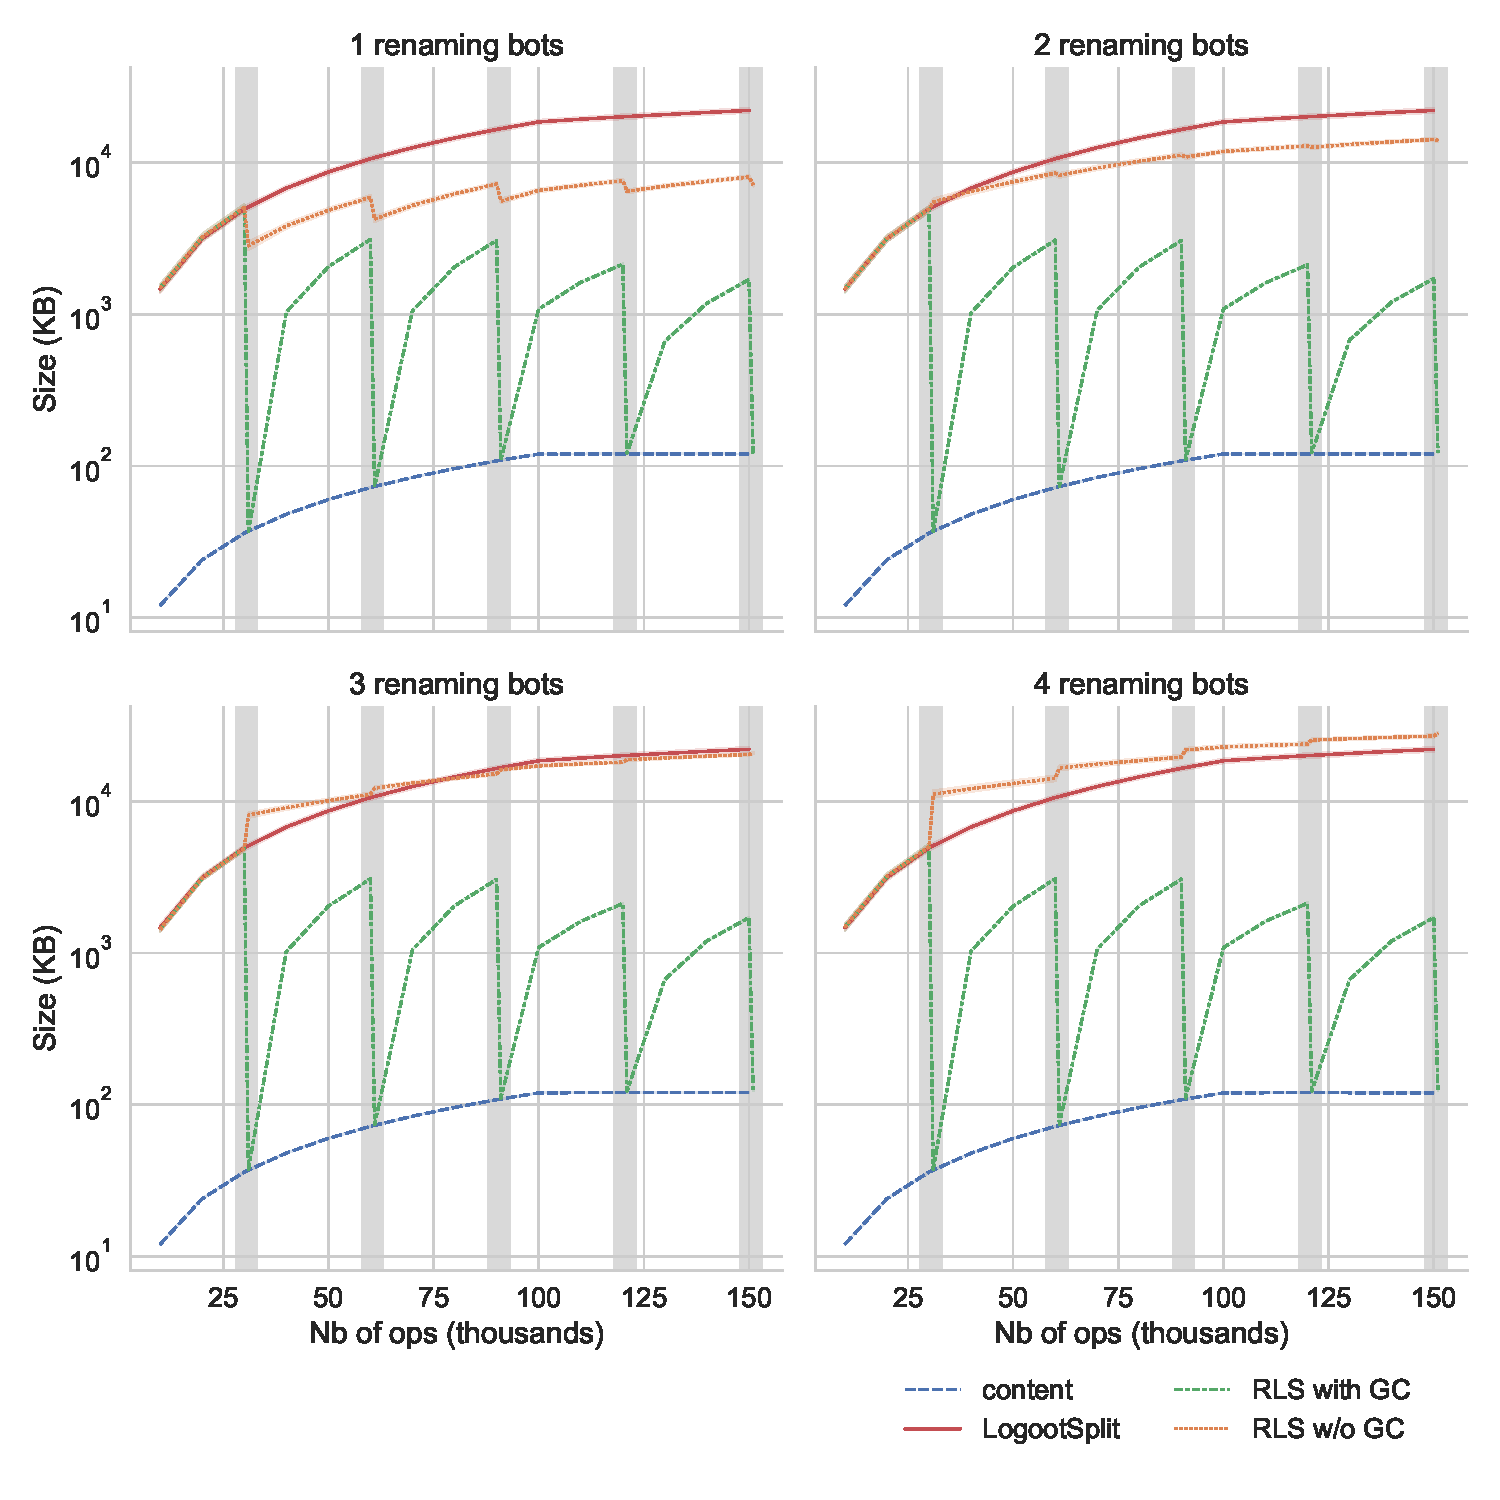
\includegraphics[width=\columnwidth]{img/2022-10-27-snapshot-sizes.pdf}
  \caption{Évolution de la taille du document en fonction du \ac{CRDT} utilisé et du nombre de \emph{renaming bots} dans la collaboration}
  \label{fig:evolution-document-size}
\end{figure}

Pour chaque graphique dans la \autoref{fig:evolution-document-size}, nous représentons les données suivantes.
Les barres grises représentent quand des opérations $\trm{rename}$ sont effectuées, \ie aux paliers de 30k, 60k, 90k, 120k et 150k opérations.
La ligne tiretée bleue correspond à la taille du contenu du document, \ie du texte, tandis que la ligne continue rouge représente la taille complète du document LogootSplit.

La ligne verte pointillée-tiretée représente la taille du document RenamableLogootSplit dans son meilleur cas.
Dans ce scénario, les noeuds considèrent que les opérations $\trm{rename}$ sont causalement stables dès qu'ils les reçoivent.
Les noeuds peuvent alors bénéficier des effets du mécanisme de renommage tout en supprimant les métadonnées qu'il introduit : les \emph{anciens états} et époques.
Ce faisant, les noeuds peuvent minimiser de manière périodique le surcoût en métadonnées de la structure de données, indépendamment du nombre de \emph{renaming bots} et d'opérations $\trm{rename}$ concurrentes générées.

La ligne pointillée orange représente la taille du document RenamableLogootSplit dans son pire cas.
Dans ce scénario, les noeuds considèrent que les opérations $\trm{rename}$ ne deviennent jamais causalement stables.
Les noeuds doivent alors conserver de façon permanente les métadonnées introduites par le mécanisme de renommage.
Les performances de RenamableLogootSplit diminuent donc au fur et à mesure que le nombre de \emph{renaming bots} et d'opérations $\trm{rename}$ générées augmente.
Néanmoins, même dans ces conditions, nous observons que RenamableLogootSplit offre de meilleures performances que LogootSplit tant que le nombre de \emph{renaming bots} reste faible (1 ou 2).
Ce résultat s'explique par le fait que le mécanisme de renommage permet aux noeuds de supprimer les métadonnées de la structure de données utilisée en interne pour représenter la séquence (\ie l'arbre AVL).

Pour récapituler les résultats présentés, le mécanisme de renommage introduit un surcoût temporaire en métadonnées qui augmente avec chaque opération $\trm{rename}$.
Mais ce surcoût se résorbe à terme une fois que le système devient quiescent et que les opérations $\trm{rename}$ deviennent causalement stables.
Dans la \autoref{sec:offloading-former-states}, nous détaillerons l'idée que les \emph{anciens états} peuvent être déchargés sur le disque en attendant que la stabilité causale soit atteinte pour atténuer l'impact du surcoût temporaire en métadonnées.




\subsubsection{Temps d'intégration des opérations standards}
Nous avons ensuite comparé l'évolution du temps d'intégration des opérations standards, \ie les opérations \emph{insert} et \emph{remove}, sur des documents LogootSplit et RenamableLogootSplit.
Puisque les deux types d'opérations partagent la même complexité en temps, nous avons seulement utilisé des opérations \emph{insert} dans nos benchmarks.
Nous faisons par contre la différence entre les mises à jours \emph{locales} et \emph{distantes}.
Conceptuellement, les modifications locales peuvent être décomposées comme présenté dans \cite{baquero2017pure} en les deux étapes suivantes :
\begin{enumerate}
  \item la génération de l'opération correspondante
  \item l'application de l'opération correspondante sur l'état local.
\end{enumerate}
Cependant, pour des raisons de performances, nous avons fusionné ces deux étapes dans notre implémentation.
Nous distinguons donc les résultats des modifications \emph{locales} et des modifications \emph{distantes} dans nos benchmarks.
La \autoref{fig:evolution-integration-time-insert} présente les résultats obtenus.

\begin{figure}[!ht]
  \centering
  \subfloat[Modifications locales]{
      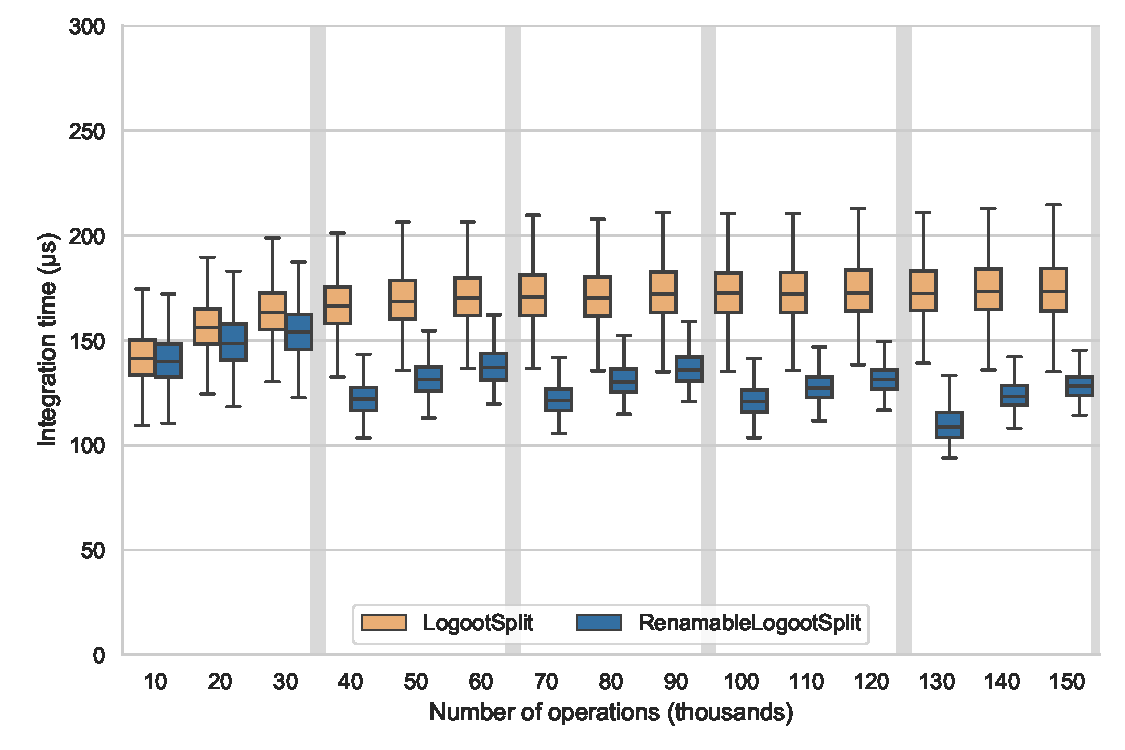
\includegraphics[width=0.45\columnwidth]{img/integration-time-boxplot-local-operations-without-outliers.pdf}
      \label{fig:evolution-integration-time-local-insert}}
  \hfil
  \subfloat[Modifications distantes]{
      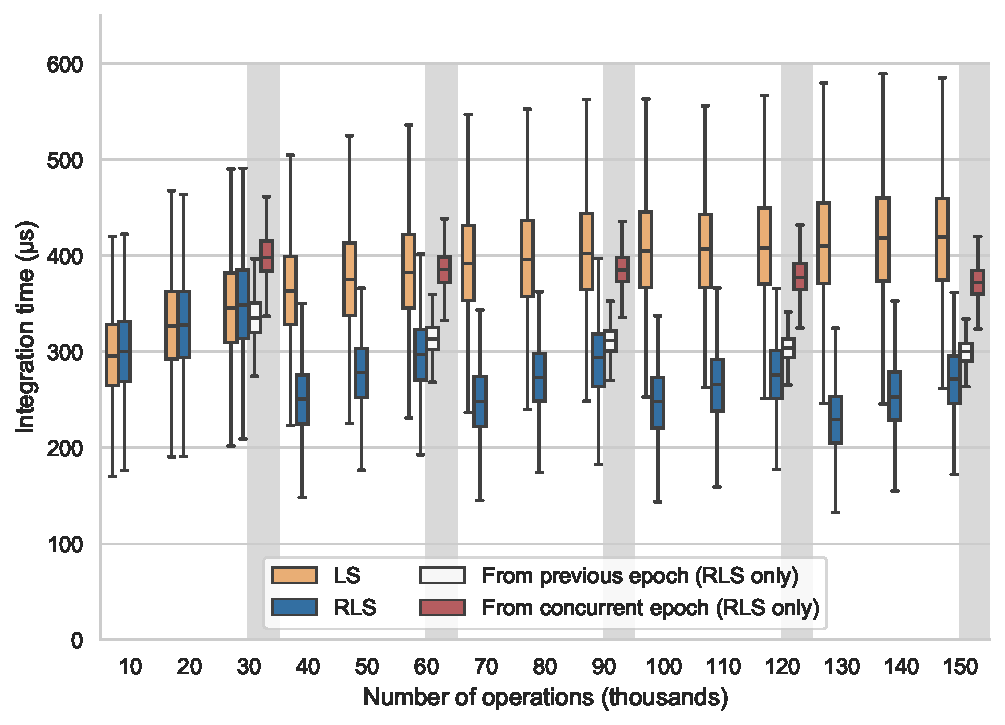
\includegraphics[width=0.45\columnwidth]{img/integration-time-boxplot-remote-operations-without-outliers.pdf}
      \label{fig:evolution-integration-time-remote-insert}}
  \caption{Temps d'intégration des opérations standards}
  \label{fig:evolution-integration-time-insert}
\end{figure}

Dans ces figures, les boxplots oranges correspondent aux temps d'intégration sur des documents LogootSplit, les boxplots bleues sur des documents RenamableLogootSplit.
Bien que les temps d'intégration soient initialement équivalents, les temps d'intégration sur des documents RenamableLogootSplit sont ensuite réduits par rapport à ceux de LogootSplit une fois que des opérations \emph{rename} ont été intégrées.
Cette amélioration s'explique par le fait que l'opération \emph{rename} optimise la représentation interne de la séquence (\ie elle réduit le nombre de blocs stockés dans l'arbre AVL).

Dans le cadre des opérations distantes, nous avons mesuré des temps d'intégration spécifiques à RenamableLogootSplit : le temps d'intégration d'opérations distantes provenant d'époques \emph{parentes} et d'époques \emph{soeurs}, respectivement affiché sous la forme de boxplots blanches et rouges dans la \autoref{fig:evolution-integration-time-remote-insert}.

Les opérations distantes provenant d'époques \emph{parentes} sont des opérations générées de manière concurrente à l'opération \emph{rename} mais appliquées après cette dernière.
Puisque l'opération doit être transformée au préalable en utilisant \textsc{renameId}, nous observons un surcoût computationnel par rapport aux autres opérations.
Mais ce surcoût est compensé par l'optimisation de la représentation interne de la séquence effectuée par l'opération \emph{rename}.

Concernant les opérations provenant d'époques \emph{soeurs}, nous observons de nouveau un surcoût puisque les noeuds doivent tout d'abord annuler les effets de l'opération \emph{rename} concurrente en utilisant \textsc{revertRenameId}.
À cause de cette étape supplémentaire, les performances de RenamableLogootSplit pour ces opérations sont comparables à celles de LogootSplit.

Pour récapituler, les fonctions de transformation ajoutent un surcoût aux temps d'intégration des opérations concurrentes aux opérations \emph{rename}.
Malgré ce surcoût, RenamableLogootSplit offre de meilleures performances que LogootSplit pour intégrer ces opérations grâce aux réductions de la taille de l'état effectuées par les opérations \emph{rename}.
Cependant, cette affirmation n'est vraie que tant que la distance entre l'époque de génération de l'opération et l'époque courante du noeud reste limitée, puisque les performances de RenamableLogootSplit dépendent linéairement de cette dernière (cf. \autoref{tab:time-complexity-operations}).
Néanmoins, ce surcoût ne concerne que les opérations concurrentes aux opérations \emph{rename}.
Il ne concerne pas la majorité des opérations, \ie les opérations générées entre deux séries d'opérations \emph{rename}.
Ces opérations, elles, ne souffrent d'aucun surcoût tout en bénéficiant des réductions de taille de l'état.


\subsubsection{Temps d'intégration de l'opération de renommage}
\label{sec:integration-time-rename}

Finalement, nous avons mesuré l'évolution du temps d'intégration de l'opération $\trm{rename}$ en fonction du nombre d'opérations émises précédemment, \ie en fonction de la taille de l'état.
Comme précédemment, nous distinguons les performances des modifications \emph{locales} et \emph{distantes}.

Nous rappellons que le traitement d'une opération $\trm{rename}$ dépend de l'ordre défini par la relation \emph{priority} entre l'époque qu'elle introduit et l'époque courante du noeud qui intègre l'opération.
Le cas des opérations $\trm{rename}$ distantes se décompose donc en trois catégories.
Les opérations \emph{distantes directes} désignent les opérations $\trm{rename}$ distantes qui introduisent une nouvelle époque \emph{enfant} de l'époque courante du noeud.
Les opérations \emph{concurrentes introduisant une plus grande} (resp. \emph{petite}) \emph{époque} désignent les opérations $\trm{rename}$ qui introduisent une époque \emph{soeur} de l'époque courante du noeud.
D'après la relation \emph{priority}, l'époque introduite est plus grande (resp. petite) que l'époque courante du noeud.
Les résultats obtenus sont présentés dans le \autoref{tab:evolution-integration-time-rename}.

\begin{table}[!ht]
  \centering
  \caption{Temps d'intégration de l'opération $\trm{rename}$}
  \label{tab:evolution-integration-time-rename}
  \resizebox{.8\columnwidth}{!}{
    \begin{tabular}{lrrrrrr}
      \toprule
      \multicolumn{2}{c}{Paramètres} & \multicolumn{5}{c}{Temps d'intégration (ms)} \\
      \cmidrule(lr){1-2} \cmidrule(lr){3-7}
      Type & Nb Ops (k) &  Moyenne & Médiane &    IQR & 1\textsuperscript{er} Percent. & 99\textsuperscript{ème} Percent. \\
      \midrule
      Locale & 30  & 41.8 &   38.7 &   5.66 &       37.3 &        71.7 \\
          & 60  & 78.3 &   78.2 &   1.58 &       76.2 &        81.4 \\
          & 90  &  119 &    119 &   2.17 &        116 &         124 \\
          & 120 &  144 &    144 &   3.24 &        139 &         149 \\
          & 150 &  158 &    158 &   3.71 &        153 &         164 \\
      \cmidrule{1-7}
      Distante directe & 30  &  481 &    477 &   15.2 &        454 &         537 \\
          & 60  &  982 &    978 &   28.9 &        926 &        1073 \\
          & 90  & 1491 &   1482 &   58.8 &       1396 &        1658 \\
          & 120 & 1670 &   1664 &     41 &       1568 &        1814 \\
          & 150 & 1694 &   1676 &   60.6 &       1591 &        1853 \\
      \cmidrule{1-7}
      Cc. int. plus grande époque & 30  &  644 &    644 &   16.6 &        620 &         683 \\
          & 60  & 1318 &   1316 &   26.5 &       1263 &        1400 \\
          & 90  & 1998 &   1994 &   46.6 &       1906 &        2112 \\
          & 120 & 2240 &   2233 &     54 &       2144 &        2368 \\
          & 150 & 2242 &   2234 &   63.5 &       2139 &        2351 \\
      \cmidrule{1-7}
      Cc. int. plus petite époque & 30  & 1.36 &    1.3 & 0.038 &       1.22 &        3.53 \\
          & 60  & 2.82 &   2.69 &  0.476 &       2.43 &        4.85 \\
          & 90  & 4.45 &   4.23 &    1.1 &       3.69 &        5.81 \\
          & 120 & 5.33 &    5.1 &   1.34 &       4.42 &        8.78 \\
          & 150 & 5.53 &   5.26 &   1.05 &       4.84 &         8.7 \\
      \bottomrule
    \end{tabular}
  }
\end{table}

Le principal résultat de ces mesures est que les opérations $\trm{rename}$ sont particulièrement coûteuses quand comparées aux autres types d'opérations.
Les opérations $\trm{rename}$ locales s'intègrent en centaines de millisecondes tandis que les opérations \emph{distantes directes} et \emph{concurrentes introduisant une plus grande époque} s'intègrent en secondes lorsque la taille du document dépasse 40k éléments.
Ces résultats s'expliquent facilement par la complexité en temps de l'opération $\trm{rename}$ qui dépend supra-linéairement du nombre de blocs et d'éléments stockés dans l'état (cf. \autoref{tab:time-complexity-operations}).
Il est donc nécessaire de prendre en compte ce résultat et de
\begin{enumerate}
  \item Concevoir des stratégies de génération des opérations $\trm{rename}$ pour éviter d'impacter négativement l'expérience utilisateur.
  \item Proposer des versions améliorées des algorithmes \textsc{renameId} et \textsc{revertRenameId} pour réduire ces temps d'intégration.
\end{enumerate}

Nous identifions plusieurs pistes d'amélioration de \textsc{renameId} et \textsc{revertRenameId} :
\begin{itemize}
  \item Au lieu d'utiliser \textsc{renameId}, qui renomme l'état identifiant par identifiant, nous pourrions définir et utiliser \textsc{renameBlock}.
    Cette fonction permettrait de renommer l'état bloc par bloc, offrant ainsi une meilleur complexité en temps.
    De plus, puisque les opérations $\trm{rename}$ fusionnent les blocs existants en un unique bloc, \textsc{renameBlock} permettrait de mettre en place un cercle vertueux où chaque opération $\trm{rename}$ réduirait le temps d'exécution de la suivante.
  \item Puisque chaque appel à \textsc{revertRenameId} et \textsc{revertRenameId} est indépendant des autres, ces fonctions sont adaptées à la programmation parallèle.
    Au lieu de renommer les identifiants (ou blocs) de manière séquentielle, nous pourrions diviser la séquence en plusieurs parties et les renommer en parallèle.
\end{itemize}

Un autre résultat intéressant de ces benchmarks est que les opérations \emph{concurrentes introduisant une plus petite époque} sont rapides à intégrer.
Puisque ces opérations introduisent une époque qui n'est pas sélectionnée comme nouvelle époque cible, les noeuds ne procèdent pas au renommage de leur état.
L'intégration des opérations \emph{concurrentes introduisant une plus petite époque} consiste simplement à ajouter l'époque introduite et l'\emph{ancien état} correspondant à l'\emph{arbre des époques}.
Les noeuds peuvent donc réduire de manière significative le coût d'intégration d'un ensemble d'opérations $\trm{rename}$ concurrentes en les appliquant dans l'ordre le plus adapté en fonction du contexte.
Nous développons ce sujet dans la \autoref{sec:report-transition-to-target-epoch}.


\subsubsection{Temps pour rejouer le journal des opérations}
Afin de comparer les performances de RenamableLogootSplit et de LogootSplit de manière globale, nous avons mesuré le temps nécessaire pour un nouveau noeud pour rejouer l'entièreté du journal des opérations d'une session de collaboration, en fonction du nombre de \emph{renaming bots} de la session.
Nous présentons les résultats obtenus dans la \autoref{fig:time-to-replay-log}.

\begin{figure}[!ht]
  \centering
  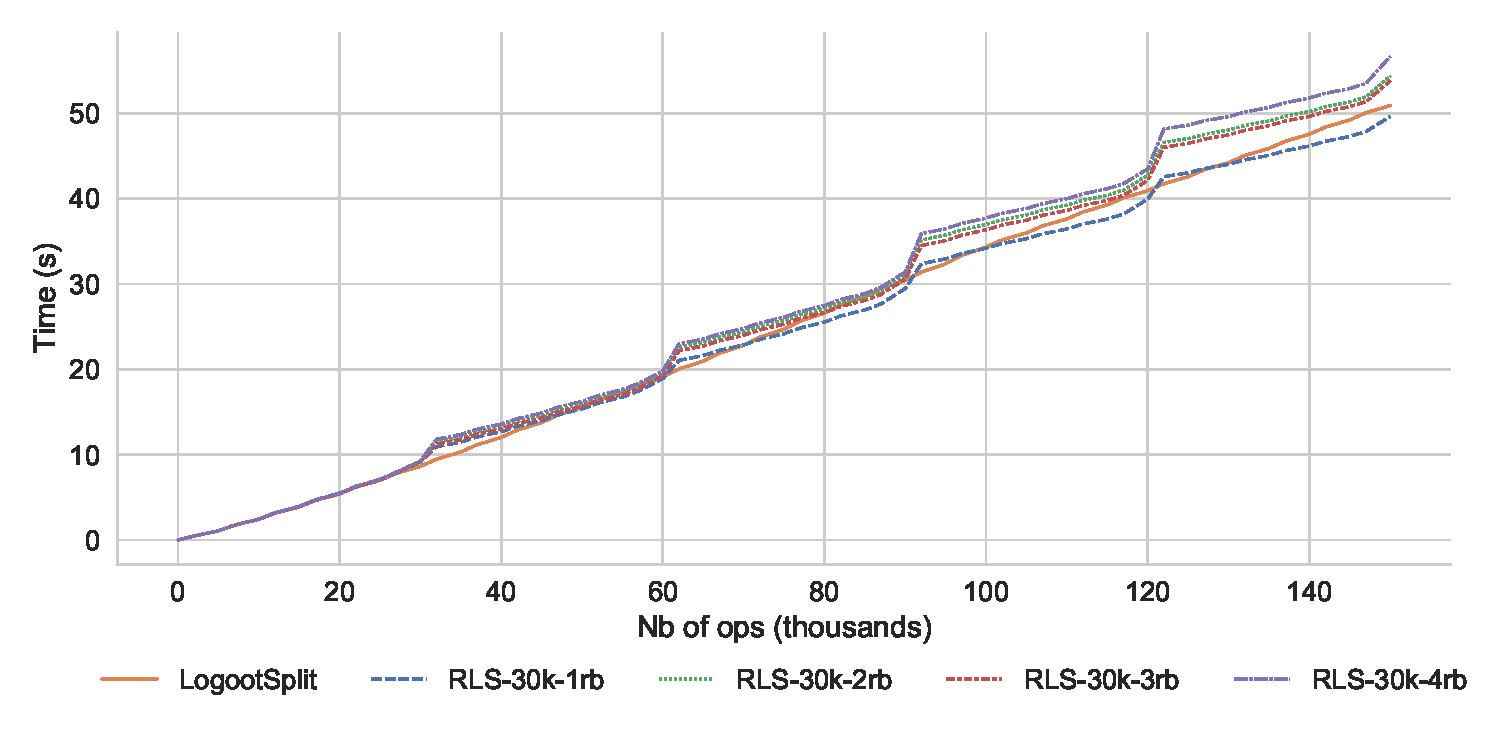
\includegraphics[width=\columnwidth]{img/replay-log-30k-2022-10-27}
  \caption{Progression du nombre d'opérations du journal rejouées en fonction du temps}
  \label{fig:time-to-replay-log}
\end{figure}

Nous observons que le gain sur le temps d'intégration des opérations $\trm{insert}$ et $\trm{remove}$ permet initialement de contrebalancer le surcoût des opérations $\trm{rename}$.
Mais au fur et à mesure que la collaboration progresse, le temps nécessaire pour intégrer les opérations $\trm{rename}$ augmente car plus d'éléments sont impliqués.
Cette tendance est accentuée dans les scénarios avec des opérations $\trm{rename}$ concurrentes.

Dans un cas réel d'utilisation, ce scénario (\ie rejouer l'entièreté du log) ne correspond pas au scénario principal et peut être mitigé, par exemple en utilisant un mécanisme de compression du journal des opérations.
Dans la \autoref{sec:rename-as-compression-mechanism}, nous présentons comment mettre en place un tel mécanisme en se basant justement sur les possibilités offertes par l'opération $\trm{rename}$.


\subsubsection{Impact de la fréquence de l'opération $\trm{rename}$ sur les performances}
Pour évaluer l'impact de la fréquence de l'opération $\trm{rename}$ sur les performances, nous avons réalisé un benchmark supplémentaire.
Ce benchmark consiste à rejouer les logs d'opérations des simulations en utilisant divers \acp{CRDT} et configurations : LogootSplit, RenamableLogootSplit effectuant des opérations $\trm{rename}$ toutes les 30k opérations, RenamableLogootSplit effectuant des opérations $\trm{rename}$ toutes les 7.5k opérations.
Au fur et à mesure que le benchmark rejoue le journal des opérations, il mesure le temps d'intégration des opérations ainsi que leur taille.
Nous présentons les résultats obtenus dans le \autoref{tab:impact-frequency-time} et le \autoref{tab:impact-frequency-memory}.

\begin{table}[!ht]
  \centering
  \resizebox{0.8\linewidth}{!}{
    \begin{tabular}{llrrrrr}
      \toprule
      \multicolumn{2}{c}{Paramètres} & \multicolumn{5}{c}{Temps d'intégration ($\trm{\mu}$s)} \\
      \cmidrule(lr){1-2} \cmidrule(lr){3-7}
      Type & CRDT & Moyenne & Médiane &  IQR & 1\textsuperscript{er} Percent. & 99\textsuperscript{ème} Percent. \\
      \midrule
      insert & LS &  471 &    460 &  130 &        224 &         768 \\
      & RLS - 30k &  397 &    323 & 66.7 &        171 &         587 \\
      & RLS - 7.5k &  393 &    265 & 54.5 &        133 &         381 \\
      remove & LS &  280 &    270 & 71.4 &        140 &         435 \\
      & RLS - 30k &  247 &    181 &   39 &       97.9 &         308 \\
      & RLS - 7.5k &  296 &    151 & 34.8 &       74.9 &         214 \\
      \midrule
      \multicolumn{2}{c}{Paramètres} & \multicolumn{5}{c}{Temps d'intégration (ms)} \\
      \cmidrule(lr){1-2} \cmidrule(lr){3-7}
      Type & CRDT & Moyenne & Médiane &  IQR & 1\textsuperscript{er} Percent. & 99\textsuperscript{ème} Percent. \\
      \midrule
      rename & RLS - 30k & 1022 &   1188 &  425 &        540 &        1276 \\
      & RLS - 7.5k &  861 &    974 &  669 &        123 &        1445 \\
      \bottomrule
    \end{tabular}
  }
  \caption{Temps d'intégration par type et par fréquence d'opérations $\trm{rename}$}
  \label{tab:impact-frequency-time}
\end{table}

D'après les résultats du \autoref{tab:impact-frequency-time}, nous observons que des opérations $\trm{rename}$ plus fréquentes permettent d'améliorer les temps d'intégration des opérations $\trm{insert}$ et $\trm{remove}$.
Cela confirme les résultats attendus puisque l'opération $\trm{rename}$ réduit la taille des identifiants de la structure ainsi que le nombre de blocs composant la séquence.

Nous remarquons aussi que la fréquence n'a aucun impact significatif sur le temps d'intégration des opérations $\trm{rename}$.
Il s'agit là aussi d'un résultat attendu puisque la complexité en temps de l'implémentation de l'opération $\trm{rename}$ dépend du nombre d'éléments dans la séquence, un facteur qui n'est pas impacté par les opérations $\trm{rename}$.

\begin{table}[!ht]
  \centering
  \resizebox{0.8\linewidth}{!}{
    \begin{tabular}{llrrrrr}
      \toprule
      \multicolumn{2}{c}{Paramètres} & \multicolumn{5}{c}{Taille (o)} \\
      \cmidrule(lr){1-2} \cmidrule(lr){3-7}
      Type & CRDT & Moyenne & Médiane &  IQR & 1\textsuperscript{er} Percent. & 99\textsuperscript{ème} Percent. \\
      \midrule
      insert & LS &  593 &    584 & 184 &        216 &        1136 \\
      & RLS - 30k &  442 &    378 &  92 &        314 &         958 \\
      & RLS - 7.5k &  389 &    378 &   0 &        314 &         590 \\
      remove & LS &   632 &     618 & 184 &        250 &        1170 \\
      & RLS - 30k &    434 &    412 &   0 &        320 &         900 \\
      & RLS - 7.5k &   401 &    412 &   0 &        320 &         596 \\
      \midrule
      \multicolumn{2}{c}{Paramètres}  & \multicolumn{5}{c}{Taille (Ko)} \\
      \cmidrule(lr){1-2} \cmidrule(lr){3-7}
      Type & CRDT & Moyenne & Médiane &  IQR & 1\textsuperscript{er} Percent. & 99\textsuperscript{ème} Percent. \\
      \midrule
      rename & RLS - 30k &   1366 &   1258 & 514 &        635 &        3373 \\
      & RLS - 7.5k &      273 &    302 & 132 &        159 &         542 \\
      \bottomrule
    \end{tabular}
  }
  \caption{Taille des opérations par type et par fréquence d'opérations $\trm{rename}$}
  \label{tab:impact-frequency-memory}
\end{table}

Le \autoref{tab:impact-frequency-memory} permet d'observer que les opérations $\trm{insert}$ et $\trm{remove}$ de RenamableLogootSplit sont initialement plus lourdes que les opérations correspondantes de LogootSplit.
Ce résultat s'explique de part le fait qu'elles intègrent leur époque de génération comme donnée additionnelle.
Mais alors que la taille des opérations de LogootSplit augmentent indéfiniment, celle des opérations de RenamableLogootSplit est bornée.
La valeur de cette borne est définie par la fréquence de l'opération $\trm{rename}$.
Cela permet à RenamableLogootSplit d'atteindre un coût moindre par opération.\\

D'un autre côté, le coût des opérations $\trm{rename}$ est bien plus important (1000x) que celui des autres types d'opérations.
Ceci s'explique par le fait que l'opération $\trm{rename}$ intègre l'\emph{ancien état}, \ie la liste de tous les blocs composant l'état de la séquence au moment de la génération de l'opération.
Cependant, nous observons le même phénomène pour les opérations $\trm{rename}$ que pour les autres opérations : la fréquence des opérations $\trm{rename}$ permet d'établir une borne pour la taille des opérations $\trm{rename}$.
Nous pouvons donc choisir d'émettre fréquemment des opérations $\trm{rename}$ pour limiter leur taille respective.
Ceci implique néanmoins un surcoût en calculs pour chaque opération $\trm{rename}$ dans l'implémentation actuelle.
Nous présentons une autre approche possible pour limiter la taille des opérations $\trm{rename}$ dans la \autoref{sec:compression-rename}.
Cette approche consiste à implémenter un mécanisme de compression pour les opérations $\trm{rename}$ pour ne transmettre que les composants nécessaires à l'identifiant de chaque bloc de l'\emph{ancien état}.


\section{Discussion}

\mnnote{TODO:
  Ajouter une partie sur la discussion qu'on a pu avoir avec les reviewers sur la présence de pierres tombales dans RenamableLogootSplit, et comment ces pierres tombales diffèrent de celles présentent dans WOOT et RGA.
}

\subsection{Stratégie de génération des opérations $\trm{rename}$}
Comme indiqué dans la \autoref{sec:def-rename-op}, les opérations \emph{rename} sont des opérations systèmes.
C'est donc aux concepteurs de systèmes qu'incombe la responsabilité de déterminer quand les noeuds devraient générer des opérations \emph{rename} et de définir une stratégie correspondante.
Il n'existe cependant pas de solution universelle, chaque système ayant ses particuliarités et contraintes.

Plusieurs aspects doivent être pris en compte lors de la définition de la stratégie de génération des opérations \emph{rename}.
Le premier porte sur la taille de la structure de données.
Comme illustré dans la \autoref{fig:evolution-document-size}, les métadonnées augmentent de manière progressive jusqu'à représenter 99\% de la structure de données.
En utilisant les opérations \emph{rename}, les noeuds peuvent supprimer les métadonnées et ainsi réduire la taille de la structure à un niveau acceptable.
Pour déterminer quand générer des opérations \emph{rename}, les noeuds peuvent donc monitorer le nombre d'opérations effectuées depuis la dernière opération \emph{rename}, le nombre de blocs qui composent la séquence ou encore la taille des identifiants.

Un second aspect à prendre en compte est le temps d'intégration des opérations \emph{rename}.
Comme indiqué dans le \autoref{tab:evolution-integration-time-rename}, l'intégration des opérations \emph{rename} distantes peut nécessiter des secondes si elles sont retardées trop longtemps.
Bien que les opérations \emph{rename} travaillent en coulisses, elles peuvent néanmoins impacter négativement l'expérience utilisateur.
Notamment, les noeuds ne peuvent pas intégrer d'autres opérations \emph{distantes} tant qu'ils sont en train de traiter des opérations \emph{rename}.
Du point de vue des utilisateurs, les opérations \emph{rename} peuvent alors être perçues comme des pics de latence.
Dans le domaine de l'édition collaborative temps réel, \textcite{2014-effect-delay-collaborative-editing-ignat,2015-cope-delay-collaborative-note-taking-ignat} ont montré que le délai dégradait la qualité des collaborations.
Il est donc important de générer fréquemment des opérations \emph{rename} pour conserver leur temps d'intégration sous une limite perceptible.

Finalement, le dernier aspect à considérer est le nombre d'opérations \emph{rename} concurrentes.
La \autoref{fig:evolution-document-size} montre que les opérations \emph{rename} concurrentes accroissent la taille de la structure de données tandis que la \autoref{fig:time-to-replay-log} illustre qu'elles augmentent le temps nécessaire pour rejouer le log d'opérations.
La stratégie proposée doit donc viser à minimiser le nombre d'opérations \emph{rename} concurrentes générées.
Cependant, elle doit éviter d'utiliser des coordinations synchrones entre les noeuds pour cela (\eg algorithmes de consensus), pour des raisons de performances.
Pour réduire la probabilité de générer des opérations \emph{rename} concurrentes, plusieurs méthodes peuvent être proposées.
Par exemple, les noeuds peuvent monitorer à quels autres noeuds ils sont connectés actuellement et déléguer au noeud ayant le plus grand \emph{identifiant de noeud} la responsabilité de générer les opérations \emph{rename}.

Pour récapituler, nous pouvons proposer plusieurs stratégies de génération des opérations \emph{rename}, pour minimiser de manière individuelle chacun des paramètres présentés.
Mais bien que certaines de ces stratégies convergent (minimiser la taille de la structure de données et minimiser le temps d'intégration des opérations \emph{rename}), d'autres entrent en conflit (générer une opération \emph{rename} dès qu'un seuil est atteint vs. minimiser le nombre d'opérations \emph{rename} concurrentes générées).
Les concepteurs de systèmes doivent proposer un compromis entre les différents paramètres en fonction des contraintes du système concerné (application temps réel ou asynchrone, limitations matérielles des noeuds...).
Il est donc nécessaire d'analyser le système pour évaluer ses performances sur chaque aspect, ses usages et trouver le bon compromis entre tous les paramètres de la stratégie de renommage.
Par exemple, dans le contexte des systèmes d'édition collaborative temps réel, \cite{2014-effect-delay-collaborative-editing-ignat} a montré que le délai diminue la qualité de la collaboration.
Dans de tels systèmes, nous viserions donc à conserver le temps d'intégration des opérations (en incluant les opérations \emph{rename}) en dessous du temps limite correspondant à leur perception par les utilisateurs.


\subsection{Stockage des états précédents sur disque}
\label{sec:offloading-former-states}
Les noeuds doivent conserver les \emph{anciens états} associés aux opérations $\trm{rename}$ pour transformer les opérations issues d'époques précédentes ou concurrentes.
Les noeuds peuvent recevoir de telles opérations dans deux cas précis :
\begin{enumerate}
  \item Des noeuds ont émis récemment des opérations $\trm{rename}$.
  \item Des noeuds se sont récemment reconnectés.
\end{enumerate}
Entre deux de ces évènements spécifiques, les \emph{anciens états} ne sont pas nécessaires pour traiter les opérations.

Nous pouvons donc proposer l'optimisation suivante : décharger les \emph{anciens états} sur le disque jusqu'à leur prochaine utilisation ou jusqu'à ce qu'ils puissent être supprimés de manière sûre.
Décharger les \emph{anciens états} sur le disque permet de mitiger le surcoût en mémoire introduit par le mécanisme de renommage.
En échange, cela augmente le temps d'intégration des opérations nécessitant un \emph{ancien état} qui a été déchargé précédemment.

Les noeuds peuvent adopter différentes stratégies, en fonction de leurs contraintes, pour déterminer les \emph{anciens états} comme déchargeables et pour les récupérer de manière préemptive.
La conception de ces stratégies peut reposer sur différentes heuristiques : les époques des noeuds actuellement connectés, le nombre de noeuds pouvant toujours émettre des opérations concurrentes, le temps écoulé depuis la dernière utilisation de l'\emph{ancien état}...


\subsection{Compression et limitation de la taille de l'opération $\trm{rename}$}
\label{sec:compression-rename}

Pour limiter la consommation en bande passante des opérations $\trm{rename}$, nous proposons la technique de compression suivante.
Au lieu de diffuser les identifiants complets formant l'\emph{ancien état}, les noeuds peuvent diffuser seulement les éléments nécessaires pour identifier de manière unique les intervalles d'identifiants.
En effet, un identifiant peut être caractérisé de manière unique par le triplet composé de l'\emph{identifiant de noeud}, du \emph{numéro de séquence} et de l'\emph{offset} de son dernier tuple.
Par conséquent, un intervalle d'identifiants peut être identifié de manière unique à partir du triplet signature de son identifiant de début et de sa longueur, \ie du quadruplet $\langle\trm{nodeId}, \trm{nodeSeq}, \trm{offsetBegin}, \trm{offsetEnd}\rangle$.
Cette méthode nous permet de réduire les données à diffuser dans le cadre de l'opération $\trm{rename}$ à un montant fixe par intervalle.

Pour décompresser l'opération reçue, les noeuds doivent reformer les intervalles d'identifiants correspondant aux quadruplets reçus.
Pour cela, ils parcourent leur état.
Lorsqu'ils rencontrent un identifiant partageant le même couple $\langle\trm{nodeId}, \trm{nodeSeq}\rangle$ qu'un des intervalles de l'opération $\trm{rename}$, les noeuds disposent de l'ensemble des informations requises pour le reconstruire.
Cependant, certains couples $\langle\trm{nodeId}, \trm{nodeSeq}\rangle$ peuvent avoir été supprimés en concurrence et ne plus être présents dans la séquence.
Dans ce cas, il est nécessaire de parcourir le journal des opérations $\trm{remove}$ concurrentes pour retrouver les identifiants correspondants et reconstruire l'opération $\trm{rename}$ originale.

Grâce à cette méthode de compression, nous pouvons instaurer une taille maximale à l'opération $\trm{rename}$.
En effet, les noeuds peuvent émettre une opération $\trm{rename}$ dès que leur état courant atteint un nombre donné d'intervalles d'identifiants, bornant ainsi la taille du message à diffuser.


\subsection{Définition de relations de priorité pour minimiser les traitements}
\label{sec:alt-priority-relation}
Bien que la relation \emph{priority} proposée dans la \autoref{sec:priority} soit simple et garantisse que tous les noeuds désignent la même époque comme époque cible, elle introduit un surcoût computationnel significatif dans certains cas.
La \autoref{fig:worst-case-priority} présente un tel cas.

\begin{figure}[!ht]
  \subfloat[Exécution d'opérations \emph{rename} concurrentes]{
      \begin{minipage}{\linewidth}
          \centering
          \resizebox{.7\linewidth}{!}{
            \begin{tikzpicture}
              \path
                node {\textbf{A}}
                ++(0:0.5) node (a0) {}
                ++(0:1) node[point, label=above:{rename to \epoch{A1}}] (a1) {}
                ++(0:2) node (a-receives-b7) {}
                ++(0:1) node [point, label=above:{rename to \epoch{A10}}] (a10) {}
                ++(0:1) node (a11) {}
                ++(0:1) node (a99) {}
                ++(0:1) node[point, label=above:{rename to \epoch{A100}}] (a100) {}
                ++(0:1.5) node (a-receives-c1) {}
                ++(0:1.5) node (a-end) {};

              \draw[thick] (a0) --  (a1) -- (a10) -- (a11);
              \draw[dotted] (a11) -- (a99);
              \draw[->, thick] (a99) -- (a100) -- (a-end);

              \path
                  ++(270:2) node {\textbf{B}}
                  ++(0:0.5) node (b0) {}
                  ++(0:2) node (b-receives-a1) {}
                  ++(0:0.5) node[point, label=below:{rename to \epoch{B2}}] (b7) {}
                  ++(0:2.5) node (b8) {}
                  ++(0:1) node (b99) {}
                  ++(0:2.5) node (b-receives-a100) {}
                  ++(0:1.5) node (b-end) {};

              \draw[thick] (b0) -- (b7) -- (b8);
              \draw[dotted] (b8) -- (b99);
              \draw[->, thick] (b99) -- (b-end);

              \path
                  ++(270:4) node {\textbf{C}}
                  ++(0:0.5) node (c0) {}
                  ++(0:2) node[point, label=below:{rename to \epoch{C1}}] (c1) {}
                  ++(0:3) node (c2) {}
                  ++(0:1) node (c99) {}
                  ++(0:4) node (c-end) {};

                \draw[thick] (c0) -- (c1) -- (c2);
                \draw[dotted] (c2) -- (c99);
                \draw[->, thick] (c99) -- (c-end);

              \draw[->, dashed, shorten >= 1] (a1) -- (b-receives-a1);
              \draw[->, dashed, shorten >= 1] (b7) -- (a-receives-b7);
              % \draw[->, dashed, shorten >= 1] (a100) -- (b-receives-a100);
              \draw[->, dashed, shorten >= 1] (c1) -- (a-receives-c1);
            \end{tikzpicture}
          }
          \label{fig:worst-case-priority-execution}
      \end{minipage}}
  \hfil
  \subfloat[\emph{Arbre des époques} final correspondant avec la relation \emph{priority} illustrée]{
      \begin{minipage}{\linewidth}
          \centering
          \resizebox{.15\linewidth}{!}{
            \begin{tikzpicture}
                \path
                    node[op] (e0) {\epoch{0}}
                    ++(225:1.5) node[op] (eA1) {\epoch{A1}}
                    ++(270:1.5) node[op] (eB7) {\epoch{B7}}
                    ++(270:1.5) node[op] (eA10) {\epoch{A10}}
                    ++(270:1) node (eA11) {}
                    ++(270:0.5) node (eA99) {}
                    ++(270:1) node[op] (eA100) {\epoch{A100}};
                \path
                    ++(315:1.5) node[op, red] (eC1) {\epoch{C1}};

                \draw[->, thick] (e0) edge (eA1) (eA1) edge (eB7) (eB7) edge (eA10) (eA10) edge (eA11) (eA99) edge(eA100) (e0) edge (eC1);
                \draw[dotted] (eA11) edge (eA99);
                \draw[->, dashed, thick, red] (eC1.270) -- (eA100.45) (eA100.50) -- (eA10.315) (eA10.45) -- (eB7.315) (eB7.45) -- (eA1.315) (eA1.0) -- (e0.270);
            \end{tikzpicture}
          }
          \label{fig:worst-case-priority-tree}
      \end{minipage}}
  \caption{Livraison d'une opération \emph{rename} d'un noeud }
  \label{fig:worst-case-priority}
\end{figure}

Dans cet exemple, les noeuds A et B éditent en collaboration un document.
Au fur et à mesure de leur collaboration, ils effectuent plusieurs opérations \emph{rename}.
Cependant, après un nombre conséquent de modifications de leur part, un autre noeud C se reconnecte.
Celui-ci leur transmet sa propre opération \emph{rename}, concurrente à toutes leurs opérations.
D'après la relation \emph{priority}, nous avons \epoch{0}~\lepoch~\epoch{A1}~\lepoch~...~\lepoch~\epoch{A100}~\lepoch~\epoch{C1}.
La nouvelle époque cible étant \epoch{C1}, les noeuds A et B doivent pour l'atteindre annuler successivement l'ensemble des opérations \emph{rename} composant leur branche de l'\emph{arbre des époques}.
Ainsi, un noeud isolé peut forcer l'ensemble des noeuds à effectuer un lourd calcul.
Il serait plus efficace que, dans cette situation, ce soit seulement le noeud isolé qui doive se mettre à jour.

La relation \emph{priority} devrait donc être conçue pour garantir la convergence des noeuds, mais aussi pour minimiser les calculs effectués globalement par les noeuds du système.
Pour concevoir une relation \emph{priority} efficace, nous pourrions incorporer dans les opérations \emph{rename} des métriques qui représentent l'état du système et le travail accumulé sur le document (nombre de noeuds actuellement à l'époque \emph{parente}, nombre d'opérations générées depuis l'époque parente, taille du document...).
De cette manière, nous pourrions favoriser la branche de l'\emph{arbre des époques} regroupant les collaborateurs les plus actifs et empêcher les noeuds isolés d'imposer leurs opérations \emph{rename}.

Afin d'offrir une plus grande flexibilité dans la conception de la relation \emph{priority}, il est nécessaire de retirer la contrainte interdisant aux noeuds de rejouer une opération \emph{rename}.
Pour cela, un couple de fonctions réciproques doit être proposée pour \textsc{renameId} et \textsc{revertRenameId}.
Une solution alternative est de proposer une implémentation du mécanisme de renommage qui repose sur les identifiants originaux plutôt que sur ceux transformés, par exemple en utilisant le log des opérations.


\subsection{Report de la transition vers la nouvelle époque cible}
\label{sec:report-transition-to-target-epoch}
Comme illustré par le \autoref{tab:evolution-integration-time-rename}, intégrer des opérations \emph{rename} distantes est généralement coûteux.
Ce traitement peut générer un surcoût computationnel significatif en cas de multiples opérations \emph{rename} concurrentes.
En particulier, un noeud peut recevoir et intégrer les opérations \emph{rename} concurrentes dans l'ordre inverse défini par la relation \emph{priority} sur leur époques.
Dans ce scénario, le noeud considérerait chaque nouvelle époque introduite comme la nouvelle époque cible et renommerait son état en conséquence à chaque fois.

% \mnnote{TODO: Ajouter figure où noeud reçoit successivement plusieurs opérations \emph{rename} concurrentes et procéde au renommage de son état à chaque fois}

En cas d'un grand nombre d'opérations \emph{rename} concurrentes, nous proposons que les noeuds retardent le renommage de leur état vers l'époque cible jusqu'à ce qu'ils aient obtenu un niveau de confiance donné en l'époque cible.
Ce délai réduit la probabilité que les noeuds effectuent des traitements inutiles.
Plusieurs stratégies peuvent être proposées pour calculer le niveau de confiance en l'époque cible.
Ces stratégies peuvent reposer sur une variété de métriques pour produire le niveau de confiance, tel que le temps écoulé depuis que le noeud a reçu une opération \emph{rename} concurrente et le nombre de noeuds en ligne qui n'ont pas encore reçu l'opération \emph{rename}.

Durant cette période d'incertitude introduite par le report, les noeuds peuvent recevoir des opérations provenant d'époques différentes, notamment de l'époque cible.
Néanmoins, les noeuds peuvent toujours intégrer les opérations \emph{insert} et \emph{remove} en utilisant \textsc{renameId} et \textsc{revertRenameId} au prix d'un surcoût computationnel pour chaque identifiant.
Cependant, ce coût est négligeable (plusieurs centaines de microsecondes par identifiant d'après la \autoref{fig:evolution-integration-time-remote-insert}) comparé au coût de renommer, de manière inutile, complètement l'état (plusieurs centaines de milliseconds à des secondes complètes d'après le \autoref{tab:evolution-integration-time-rename}).

Notons que ce mécanisme nécessite que \textsc{renameId} et \textsc{revertRenameId} soient des fonctions réciproques.
En effet, au cours de la période d'incertitude, un noeud peut avoir à utiliser \textsc{revertRenameId} pour intégrer les identifiants d'opérations \emph{insert} distantes provenant de l'époque cible.
Ensuite, le noeud peut devoir renommer son état vers l'époque cible une fois que celle-ci a obtenu le niveau de confiance requis.
Il s'ensuit que \textsc{renameId} doit restaurer les identifiants précédemment transformés par \textsc{revertRenameId} à leur valeur initiale pour garantir la convergence.


\subsection{Utilisation de l'opération de renommage comme mécanisme de compression du journal des opérations}
\label{sec:rename-as-compression-mechanism}
Lorsqu'un nouveau pair rejoint la collaboration, il doit tout d'abord récupérer l'état courant du document avant de pouvoir participer.
Le nouveau pair utilise un mécanisme d'anti-entropie \cite{1983-anti-entropy-vv} pour récupérer l'ensemble des opérations via un autre pair.
Puis il reconstruit l'état courant en appliquant successivement chacune des opérations.
Ce processus peut néanmoins s'avérer coûteux pour les documents comprenant des milliers d'opérations.

Pour pallier ce problème, des mécanismes de compression du log ont été proposés dans la littérature.
Les approches présentées dans \cite{2002-log-compression-op-based-vcs-shen-sun, 2006-these-claudia} consistent à remplacer un sous-ensemble des opérations du log par une opération équivalente, par exemple en aggrégeant les opérations \emph{insert} adjacentes.
Une autre approche, présentée dans \cite{2014-making-op-based-crdts-op-based}, définie une relation \emph{obsolete} sur les opérations.
La relation \emph{obsolete} permet de spécifier qu'une nouvelle opération rend obsolètes des opérations précédentes et permet de les retirer du log.
Pour donner un exemple, une opération d'ajout d'un élément donné dans un OR-Set \ac{CRDT} rend obsolètes toutes les opérations précédentes d'ajout et de suppression de cet élément.

Dans notre contexte, il est intéressant de noter que l'opération \emph{rename} peut endosser un rôle comparable à ces mécanismes de compression du log.
En effet, l'opération \emph{rename} prend un état donné, somme des opérations passées, et génère en retour un nouvel état équivalent et compacté.
Une opération \emph{rename} rend donc obsolète l'ensemble des opérations dont elle dépend causalement, et peut être utilisée pour les remplacer.
En partant de cette observation, nous proposons le mécanisme de compression du log suivant.

Le mécanisme consiste à réduire le nombre d'opérations transmises à un nouveau pair rejoignant la collaboration grâce à l'opération \emph{rename} de l'époque courante.
L'opération \emph{rename} ayant introduite l'époque courante fournit un état initial au nouveau pair.
À partir de cet état initial, le nouveau pair peut obtenir l'état courant en intégrant les opérations \emph{insert} et \emph{remove} qui ont été générées de manière concurrente ou causale par rapport à l'opération \emph{rename}.
En réponse à une demande de synchronisation d'un nouveau pair, un pair peut donc simplement lui envoyer un sous-ensemble de son log composé de :
\begin{enumerate*}
  \item l'opération \emph{rename} ayant introduite son époque courante
  \item les opérations \emph{insert} et \emph{remove} dont l'opération \emph{rename} courante ne dépend pas causalement.
\end{enumerate*}

Notons que les données contenues dans l'opération \emph{rename} telle que nous l'avons définie précédemment (cf. \autoref{def:rename-op}) sont insuffisantes pour cette utilisation.
En effet, les données incluses (\emph{ancien état} au moment du renommage, identifiant du noeud auteur de l'opération \emph{rename} et son numéro de séquence au moment de la génération) nous permettent seulement de recréer la structure de la séquence après le renommage.
Mais le contenu de la séquence est omis, celui-ci n'étant jusqu'ici d'aucune utilité pour l'opération \emph{rename}.
Afin de pouvoir utiliser l'opération \emph{rename} comme état initial, il est nécessaire d'y inclure cette information.

De plus, des informations de causalité doivent être intégrées à l'opération \emph{rename}.
Ces informations doivent permettre aux noeuds d'identifier les opérations supplémentaires nécessaires pour obtenir l'état courant, \ie toutes les opérations desquelles l'opération \emph{rename} ne dépend pas causalement.
L'ajout à l'opération \emph{rename} d'un \emph{vecteur de version}, structure représentant l'ensemble des opérations intégrées par l'auteur de l'opération \emph{rename} au moment de sa génération, permettrait cela.

Nous définissons donc de la manière suivante l'opération \emph{rename} enrichie compatible avec ce mécanisme de compression du log :

\begin{definition}[rename enrichie]
  \label{def:-rich-rename-op}
  Une opération \emph{rename enrichie} est un quintuplet $\langle$nodeId, nodeSeq, formerState, versionVector, content$\rangle$ où
  \begin{itemize}
    \item nodeId est l'identifiant du noeud qui a générée l'opération \emph{rename}.
    \item nodeSeq est le numéro de séquence du noeud au moment de la génération de l'opération \emph{rename}.
    \item formerState est l'ancien état du noeud au moment du renommage.
    \item versionVector est le vecteur de version représentant l'ancien état du noeud au moment du renommage.
    \item content est le contenu du document au moment du renommage.
  \end{itemize}
\end{definition}

Ce mécanisme de compression du log introduit néanmoins le problème suivant.
Un nouveau pair synchronisé de cette manière ne possède qu'un sous-ensemble du log des opérations.
Si ce pair reçoit ensuite une demande de synchronisation d'un second pair, il est possible qu'il ne puisse répondre à la requête.
Par exemple, le pair ne peut pas fournir des opérations faisant partie des dépendances causales de l'opération \emph{rename} qui lui a servi d'état initial.

Une solution possible dans ce cas de figure est de rediriger le second pair vers un troisième pour qu'il se synchronise avec lui.
Cependant, cette solution pose des problèmes de latence/temps de réponse si le troisième pair s'avère indisponible à ce moment.
Une autre approche possible est de généraliser le processus de synchronisation que nous avons présenté ici (opération \emph{rename} comme état initial puis application des autres opérations) à l'ensemble des pairs, et non plus seulement aux nouveaux pairs.
Nous présentons les avantages et inconvénients de cette approche dans la sous-section suivante.

% \mnnote{TODO: Étudier si y a un intérêt à privilégier la synchronisation basée sur l'intégration successive de toutes les opérations quand on a cette méthode de synchronisation par snapshot/checkpoint de possible}


\subsection{Implémentation alternative de l'intégration de l'opération $\trm{rename}$ basée sur le journal des opérations}
\label{sec:log-based-rename-mechanism}
Nous avons décrit précédemment dans la \autoref{sec:integration-process-rename-op}, et plus précisément dans l'\autoref{alg:renameRemote}, le processus d'intégration de l'opération \emph{rename} évaluée dans ce manuscrit.
Pour rappel, le processus consiste à
\begin{enumerate*}
  \item identifier le chemin entre l'époque courante et l'époque cible
  \item appliquer les fonctions de transformations \textsc{revertRenameId} et \textsc{renameId} à l'ensemble des identifiants composant l'état courant
  \item re-créer une séquence à partir des nouveaux identifiants calculés et du contenu courant.
\end{enumerate*}

Dans cette section, nous abordons une implémentation alternative de l'intégration de l'opération \emph{rename}.
Cette implémentation repose sur le log des opérations.

Cette implémentation se base sur les observations suivantes :
\begin{enumerate*}
  \item L'état courant est obtenu en intégrant successivement l'ensemble des opérations.
  \item L'opération \emph{rename} est une opération subsumant les opérations passées : elle prend un état donné (l'\emph{ancien état}), somme des opérations précédentes, et génère un nouvel état équivalent compacté.
  \item L'ordre d'intégration des opérations concurrentes n'a pas d'importance sur l'état final obtenu.
\end{enumerate*}

Ainsi, pour intégrer une opération \emph{rename} distante, un noeud peut
\begin{enumerate*}
  \item générer l'état correspondant au renommage de l'\emph{ancien état}
  \item identifier le chemin entre l'époque courante et l'époque cible
  \item identifier les opérations concurrentes à l'opération \emph{rename} présentes dans son log
  \item transformer et intégrer successivement les opérations concurrentes à l'opération \emph{rename} à ce nouvel état
\end{enumerate*}

Cet algorithme est équivalent à ré-ordonner le log des opérations de façon à intégrer les opérations précédant l'opération \emph{rename}, puis à intégrer l'opération \emph{rename} elle-même, puis à intégrer les opérations concurrentes à cette dernière.

Cette approche présente plusieurs avantages par rapport à l'implémentation décrite dans la \autoref{sec:integration-process-rename-op}.
Tout d'abord, elle modifie le facteur du nombre de transformations à effectuer.
La version décrite dans la \autoref{sec:integration-process-rename-op} transforme de l'époque courante vers l'époque cible chaque identifiant (ou chaque bloc si nous disposons de \textsc{renameBlock}) de l'état courant.
La version présentée ici effectue une transformation pour chaque opération du log concurrente à l'opération \emph{rename} à intégrer.
Le nombre de transformation peut donc être réduit de plusieurs ordres de grandeur avec cette approche, notamment si les opérations sont propagées aux pairs du réseau rapidement.

Un autre avantage de cette approche est qu'elle permet de récupérer et de réutiliser les identifiants originaux des opérations.
Lorsqu'une suite de transformations est appliquée sur les identifiants d'une opération, elle est appliquée sur les identifiants originaux et non plus sur leur équivalents présents dans l'état courant.
Ceci permet de réinitialiser les transformations appliquées à un identifiant et d'éviter le cas de figure mentionné dans la \autoref{sec:reverting-rename-ops} : le cas où \textsc{revertRenameId} est utilisé pour retirer l'effet d'une opération \emph{rename} sur un identifiant, avant d'utiliser \textsc{renameId} pour ré-intégrer l'effet de la même opération \emph{rename}.
Cette implémentation supprime donc la contrainte de définir un couple de fonctions réciproques \textsc{renameId} et \textsc{revertRenameId}, ce qui nous offre une plus grande flexibilité dans le choix de la relation \lepoch et du couple de fonctions \textsc{renameId} et \textsc{revertRenameId}.

Cette implémentation dispose néanmoins de plusieurs limites.
Tout d'abord, elle nécessite que chaque noeud maintienne localement le log des opérations.
Les métadonnées accumulées par la structure de données répliquées vont alors croître avec le nombre d'opérations effectuées.
Cependant, ce défaut est à nuancer.
En effet, les noeuds doivent déjà maintenir le log des opérations pour le mécanisme d'anti-entropie, afin de renvoyer une opération passée à un noeud l'ayant manquée.
Plus globalement, les noeuds doivent aussi conserver le log des opérations pour permettre à un nouveau noeud de rejoindre la collaboration et de calculer l'état courant en rejouant l'ensemble des opérations.
Il s'agit donc d'une contrainte déjà imposée aux noeuds pour d'autres fonctionnalités du système.

Un autre défaut de cette implémentation est qu'elle nécessite de détecter les opérations concurrentes à l'opération \emph{rename} à intégrer.
Cela implique d'ajouter des informations de causalité à l'opération \emph{rename}, tel qu'un vecteur de version.
Cependant, la taille des vecteurs de version croît de façon monotone avec le nombre de noeuds qui participent à la collaboration.
Diffuser cette information à l'ensemble des noeuds peut donc représenter un coût significatif dans les collaborations à large échelle.
Néanmoins, il faut rappeler que les noeuds échangent déjà régulièrement des vecteurs de version dans le cadre du fonctionnement du mécanisme d'anti-entropie.
Les opérations \emph{rename} étant rares en comparaison, ce surcoût nous paraît acceptable.

Finalement, cette approche implique aussi de parcourir le log des opérations à la recherche d'opérations concurrentes.
Comme dit précédemment, la taille du log croît de façon monotone au fur et à mesure que les noeuds émettent des opérations.
Cette étape du nouvel algorithme d'intégration de l'opération \emph{rename} devient donc de plus en plus coûteuse.
Des méthodes permettent néanmoins de réduire son coût computationnel.
Notamment, chaque noeud traquent les informations de progression des autres noeuds afin de supprimer les métadonnées du mécanisme de renommage (cf. \autoref{sec:gc-mechanism}).
Ces informations permettent de déterminer la stabilité causale des opérations et donc d'identifier les opérations qui ne peuvent plus être concurrentes à une nouvelle opération \emph{rename}.
Les noeuds peuvent ainsi maintenir, en plus du log complet des opérations, un log composé uniquement des opérations non stables causalement.
Lors du traitement d'une nouvelle opération \emph{rename}, les noeuds peuvent alors parcourir ce log réduit à la recherche des opérations concurrentes.


\mnnote{TODO: Ajouter conclusion à cette sous-section}

\section{Comparaison avec les approches existantes}

\subsection{Core-Nebula}
\cite{letia:hal-01248270} puis \cite{zawirski:hal-01248197} définissent un mécanisme de ré-équilibrage de l'arbre des identifiants de position pour Treedoc \cite{2009-treedoc-preguica}.
Ce mécanisme, qui prend la forme d'une nouvelle opération $\trm{rebalance}$, permet aux noeuds de réassigner des identifiants plus courts aux éléments du document.
Cependant, cette nouvelle opération n'est ni commutative avec les opérations $\trm{insert}$ et $\trm{remove}$, ni avec elle-même.
Pour assurer la convergence à terme \cite{10.1145/224057.224070} du système, \cite{zawirski:hal-01248197} fait le choix d'empêcher la génération d'opérations $\trm{rebalance}$ concurrentes.
Pour cela, cette approche requiert un consensus entre les noeuds pour générer les opérations $\trm{rebalance}$.
Les opérations $\trm{insert}$ et $\trm{remove}$ sont elles toujours générées sans coordination entre les noeuds et peuvent donc être concurrentes aux opérations $\trm{rebalance}$.
Pour gérer les opérations concurrentes aux opérations $\trm{rebalance}$, les auteurs proposent de transformer les opérations concernées par rapport aux effets des opérations$\trm{rebalance}$, à l'aide un mécanisme de \emph{catch-up}, avant de les appliquer.

Cependant, les protocoles de consensus ne passent pas à l'échelle et ne sont pas adaptés aux systèmes distribués à large échelle.
Pour pallier ce problème, les auteurs proposent de répartir les noeuds dans deux groupes : le \emph{core} et la \emph{nebula}.
Le \emph{core} est un ensemble, de taille réduite, de noeuds stables et hautement connectés tandis que la \emph{nebula} est un ensemble, de taille non-bornée, de noeuds.
Seuls les noeuds du \emph{core} participent à l'exécution du protocole de consensus.
Les noeuds de la \emph{nebula} contribuent toujours au document par le biais des opérations $\trm{insert}$ et $\trm{remove}$.

Notre travail peut être vu comme une extension des travaux.
Avec RenamableLogootSplit, nous adaptons l'opération $\trm{rebalance}$ et le mécanisme de \emph{catch-up} à LogootSplit pour tirer partie de la fonctionnalité offerte par les blocs.
De plus, nous proposons un mécanisme pour supporter les opérations $\trm{rename}$ concurrentes, ce qui supprime la nécessité de l'utilisation d'un protocole de consensus.
Notre contribution est donc une approche plus générique puisque RenamableLogootSplit est utilisable dans des systèmes composés d'un \emph{core} et d'une \emph{nebula}, ainsi que dans les systèmes ne disposant pas de noeuds stables pour former un \emph{core}.

Dans les systèmes disposant d'un \emph{core}, nous pouvons donc combiner RenamableLogootSplit avec un protocole de consensus pour éviter la génération d'opérations $\trm{rename}$ concurrentes.
Cette approche offre plusieurs avantages.
Elle permet de se passer de tout ce qui à attrait au support d'opérations $\trm{rename}$ concurrentes, \ie la définition d'une relation \emph{priority} et l'implémentation de \textsc{revertRenameId}.
Elle permet aussi de simplifier l'implémentation du mécanisme de récupération de mémoire des époques et \emph{anciens états} pour reposer seulement sur la stabilité causale des opérations.
Concernant ses performances, cette approche se comporte de manière similaire à RenamableLogootSplit avec un seul \emph{renaming bot} \cf{sec:evaluation-results}, mais avec un surcoût correspondant au coût du protocole de consensus sélectionné.


\subsection{LSEQ}
L'approche LSEQ \cite{lseq2013, lseq2017} est une approche visant à ralentir la croissance des identifiants dans les Séquences \acp{CRDT} à identifiants densément ordonnés.
Au lieu de réduire périodiquement la taille des métadonnées liées aux identifiants à l'aide d'un mécanisme de renommage coûteux, les auteurs définissent de nouvelles stratégies d'allocation des identifiants pour ralentir leur vitesse de croissance.
Dans ces travaux, les auteurs notent que la stratégie d'allocation des identifiants proposée dans Logoot \cite{2009-logoot-weiss} n'est adaptée qu'à un seul comportement d'édition : de gauche à droite, de haut en bas.
Si les insertions sont effectuées en suivant d'autres comportements, les identifiants générés saturent rapidement l'espace des identifiants pour une taille donnée.
Les insertions suivantes déclenchent alors une augmentation de la taille des identifiants.
En conséquent, la taille des identifiants dans Logoot augmente de façon linéaire au nombre d'insertions, au lieu de suivre la progression logarithmique attendue.

LSEQ définit donc plusieurs stratégies d'allocation d'identifiants adaptées à différents comportements d'édition.
Les noeuds choisissent aléatoirement une de ces stratégies pour chaque taille d'identifiants.
De plus, LSEQ adopte une structure d'arbre exponentiel pour allouer les identifiants : l'intervalle des identifiants possibles double à chaque fois que la taille des identifiants augmente.
Cela permet à LSEQ de choisir avec soin la taille des identifiants et la stratégie d'allocation en fonction des besoins.
En combinant les différentes stratégies d'allocation avec la structure d'arbre exponentiel, LSEQ offre une croissance polylogarithmique de la taille des identifiants en fonction du nombre d'insertions.

Bien que l'approche LSEQ ralentisse la vitesse de croissance des identifiants dans les Séquences \acp{CRDT} à identifiants densément ordonnés, le surcoût de la séquence reste proportionnel à son nombre d'éléments.
À l'inverse, le mécanisme de renommage de RenamableLogootSplit permet de réduire les métadonnées à une quantité fixe, indépendamment du nombre d'éléments.

Ces deux approches sont néanmoins orthogonales et peuvent, comme avec l'approche précédente, être combinées.
Le système résultant réinitialiserait périodiquement les métadonnées de la séquence répliquée à l'aide de l'opération $\trm{rename}$ tandis que les stratégies d'allocation d'identifiants de LSEQ ralentiraient leur croissance entretemps.
Cela permettrait aussi de réduire la fréquence de l'opération $\trm{rename}$, réduisant ainsi les calculs effectués par le système de manière globale.

% \mnnote{Serait intéressant d'avoir une implémentation combinant LogootSplit et LSEQ pour vérifier si les contraintes sur la création de blocs dans LogootSplit ne "sabotent" pas la croissance polylogarithmique des identifiants de LSEQ}



% \subsection{Eager stability determination}

% \mnnote{Peut aussi aborder les travaux de Jim Bauwens et Elisa Gonzalez Boix \cite{2019-memory-efficient-crdts-dynamic-environments-bauwens, 2020-flec-bauwens, 2020-from-causality-to-stability-reducing-metadata-crdts-bauwens} sur l'accélération de la stabilité causale : ne concerne pas seulement les séquences, mais les operation-based CRDTs. Permet de tronquer le journal des opérations mais aussi d'accélerer le mécanisme de GC de RGA (et le mien aussi)}

% \mnnote{Peut aborder les travaux de Weidner, Miller et Meiklejohn \cite{10.1145/3380787.3393687, 10.1145/3408976} qui combinent aussi CRDT et OT dans une certaine mesure. Pas vraiment dans le but de réduire les métadonnées du CRDT. Mais reste intéressant à présenter pour se différencier (eux proposent d'utiliser OT pour fusionner 2 CRDTs, moi pour ajouter une action qui est incompatible nativement avec les autres actions du CRDT)}

\section{Conclusion}

Dans ce chapitre, nous avons présenté un nouveau \ac{CRDT} pour le type Séquence : RenamableLogootSplit.
Ce nouveau type de données répliquées associe à LogootSplit un mécanisme de renommage optimiste permettant de réduire périodiquemment les métadonnées stockées et d'optimiser l'état interne de la structure de données.

Ce mécanisme prend la forme d'une nouvelle opération, l'opération $\trm{rename}$, qui peut être émise à tout moment par n'importe quel noeud.
Cette opération génère une nouvelle séquence LogootSplit, équivalente à l'état précédent, avec une empreinte minimale en métadonnées.
L'opération $\trm{rename}$ transporte aussi suffisamment d'informations pour que les noeuds puissent intégrer les opérations concurrentes à l'opération $\trm{rename}$ dans le nouvel état.

En cas d'opérations $\trm{rename}$ concurrentes, la relation d'ordre strict total \lepoch permet aux noeuds de décider quelle opération $\trm{rename}$ utiliser, sans coordination.
Les autres opérations $\trm{rename}$ sont quant à elles ignorées.
Seules leurs informations sont stockées par RenamableLogootSplit, afin de gérer les opérations concurrentes potentielles.

Une fois qu'une opération $\trm{rename}$ a été propagée à l'ensemble des noeuds, elle devient causalement stable.
À partir de ce point, il n'est plus possible qu'un noeud émette une opération concurrente à cette dernière.
Les informations incluses dans l'opération $\trm{rename}$ pour intégrer les opérations concurrentes potentielles peuvent donc être supprimées par l'ensemble des noeuds.

Ainsi, le mécanisme de renommage permet à RenamableLogootSplit d'offrir de meilleures performances que LogootSplit.
La génération du nouvel état minimal et la suppression à terme des métadonnées du mécanisme de renommage divisent par 100 la taille de la structure de données répliquée.
L'optimisation de l'état interne représentant la séquence réduit aussi le coût d'intégration des opérations suivantes, amortissant ainsi le coût de transformation et d'intégration des opérations concurrentes à l'opération $\trm{rename}$.

RenamableLogootSplit souffre néanmoins de plusieurs limitations.
La première d'entre elles est le besoin d'observer la stabilité causale des opérations $\trm{rename}$ pour supprimer de manière définitive les métadonnées associées.
Il s'agit d'une contrainte forte, notamment dans les systèmes dynamiques à grande échelle dans lesquels nous n'avons aucune garantie et aucun contrôle sur les noeuds.
Il est donc possible qu'un noeud déconnecté ne se reconnecte jamais, bloquant ainsi la progression de la stabilité causale pour l'ensemble des opérations.
Il s'agit toutefois d'une limite partagée avec les autres mécanismes de réduction des métadonnées pour Sequence \acp{CRDT} proposés dans la littérature \cite{ROH2011354, zawirski:hal-01248197}, à l'exception de l'approche LSEQ \cite{lseq2017}.
En pratique, il serait intéressant d'étudier la mise en place d'un mécanisme d'éviction des noeuds inactifs pour répondre à ce problème.
\mnnote{
  TODO: Revoir ce point pour indiquer que stabilité causale n'est pas une condition raisonnable dans systèmes sujets au churn.
  Qu'à notre sens, rend cette solution inadéquate par rapport au modèle du système.
  Mais préciser que majorité des noeuds dans ce type de système se connectent de manière éphèmère, \ie ne reviennent jamais.
  Mais principe d'une collaboration est de collaborer.
  Si noeuds ne collaborent pas ou mal, \eg font un truc dans leur coin pendant X mois (dépendant du cas d'application), nous paraît justifier de les retirer de la collaboration.
}
% Pour gérer le cas où des noeuds inactifs empêche la stabilité causale des opérations d'être atteinte, une solution possible serait de mettre en place un mécanisme d'éviction des noeuds inactifs.
% La collaboration poursuivrait alors uniquement avec les noeuds
% Cette solution est néanmoins imparfaite, car elle peut conduire à des forks,

La seconde limitation de RenamableLogootSplit concerne la génération d'opérations $\trm{rename}$ concurrentes.
Chaque opération $\trm{rename}$ est coûteuse, aussi bien en terme de métadonnées à stocker et diffuser qu'en terme de traitements à effectuer.
Il est donc important de chercher à minimiser le nombre d'opérations $\trm{rename}$ concurrentes émises par les noeuds.
Une approche possible est d'adopter une architecture du type \emph{core-nebula}\cite{zawirski:hal-01248197}.
Mais pour les systèmes incompatibles avec ce type d'architecture système, il serait intéressant de proposer d'autres approches ne nécessitant aucune coordination entre les noeuds.
Mais par définition, ces approches ne pourraient offrir de garanties fortes sur le nombre d'opérations concurrentes possibles.

